\documentclass[a4paper,12pt]{article}
\usepackage[croatian]{babel}
\usepackage[utf8]{inputenc}
\usepackage[T1]{fontenc}
\usepackage{gensymb}
\usepackage{tikz}
\usepackage{lscape}
\usepackage{amsmath,amsfonts,amssymb,mathrsfs}
\usepackage{fancyhdr,makeidx}
\usepackage{dcolumn,multirow,eucal,hhline,subcaption}
\usepackage{pgfplots,pgfplotstable,colortbl,array}
\usepackage[unicode, hidelinks]{hyperref}
\usepackage{ragged2e}
\usepackage{
epstopdf,
graphicx,tikz,
%pgflibraryshapes,
color,caption,
listings,
dcolumn,
multirow,
array,
booktabs,
picture,
upgreek,
wrapfig,      
cancel,
placeins,
url,
verbatim,
media9,
float,
incgraph
}
\usepackage[nottoc,numbib]{tocbibind}
\usepackage[croatian]{nomencl}
\makenomenclature
\usepgfplotslibrary{units}
\usetikzlibrary{pgfplots.units}
\usetikzlibrary{angles,calc,decorations.pathmorphing,patterns}
\usetikzlibrary{decorations.pathmorphing,decorations.pathreplacing}
\pgfplotstableset{precision=10,set thousands separator={}}
\usepackage{nicefrac}
\hoffset -30 pt
\voffset -50 pt
\textheight = 650 pt
\textwidth = 450 pt
\sloppy
\definecolor{lightgray}{gray}{0.5}
\setlength{\parindent}{0pt}
\usepgfplotslibrary{external}
\usetikzlibrary{pgfplots.external}
\usepgfplotslibrary{external}
\usepackage{lmodern,textcomp}
\usepackage{multimedia}
\headheight = 14 pt
\headwidth = 17 cm
\pagestyle{fancy}


\newcommand{\tikzAngleOfLine}{\tikz@AngleOfLine} %crtanje kuteva
  \def\tikz@AngleOfLine(#1)(#2)#3{%
  \pgfmathanglebetweenpoints{%
    \pgfpointanchor{#1}{center}}{%
    \pgfpointanchor{#2}{center}}
  \pgfmathsetmacro{#3}{\pgfmathresult}%
  }


\fancyfoot[R]{\thepage}
\fancypagestyle{fancypage}{
    \fancyhf{}
    \footrulewidth=20pt
    %\renewcommand{\headrulewidth}{0pt}
    \renewcommand{\footrulewidth}{0.4pt}
}
\cfoot[]{}
\renewcommand{\thefigure}{\arabic{section}.\arabic{subsection}.\arabic{figure}}
\makeindex
\numberwithin{figure}{section}
\graphicspath{ {./Dino/} }
\setlength\parindent{24pt}

\begin{document}

\begin{titlepage}
  \null\vfill

  \begin{center}

  {\huge\bfseries Obrada metala}
  \vskip 2cm
  
  \end{center}
\vfill
\hfill
\end{titlepage}
\clearpage
\tableofcontents
\clearpage
\section{Teorija rezanja metala}
\subsection{Alati za rad skidanjem strugotine}
Obrađivanje skidanjem strugotine, kao np.: rezanje, tokarenje, struganje, glodanje, brušenje, provlačenje, grecanje, vrši se raznim alatima. Jednom to može biti \textbf{nož} s jednom oštricom (tokarenje, blanjanje), drugi puta \textbf{svrdlo} koje na sebi nosi dvije osnovne oštrice, treči puta alat sa više oštrica koje odjednom skidaju strugotinu (turpija, brusna ploča). \par 
Skidanje strugotina mora, kao i ostali zahvati, odgovarati nekim zakonitostima. Te zakonitosti prvi je počeo proučavati amerikanac F.W.Taylor krajem prošlog stoljeća.\par
Svaki alat, koji koristimo pri skidanju strugotina, kao što smo vidjeli, sastoji se od jedne ili više oštrica. To nas dovodi do zaključka, da analogijom tu zakonitost prenesemo na sve druge.\par
Osnovna oštrica alata za rezanje bazira se na principu klina. Znači, moramo proučiti djelovanje klina. Zbog toga mi ćemo se zadržati na jednom alatu, a to je \textbf{tokarski nož}, te ćemo na njemu proučiti sve.
\subsection{Geometrijski oblici oštrice alata i elementi oštrine}
Rekli smo da je temeljni oblik svakog alata za rezanje klin. To vrijedi kod dljeta, kod oštrice škara, kod turpije, tokarskog noža, glodala itd. \par
Prvo da se upoznamo opčenito s tokarskim nožem i njegovim elementima rezanja i plohama.
\begin{figure}[!h]
\centering
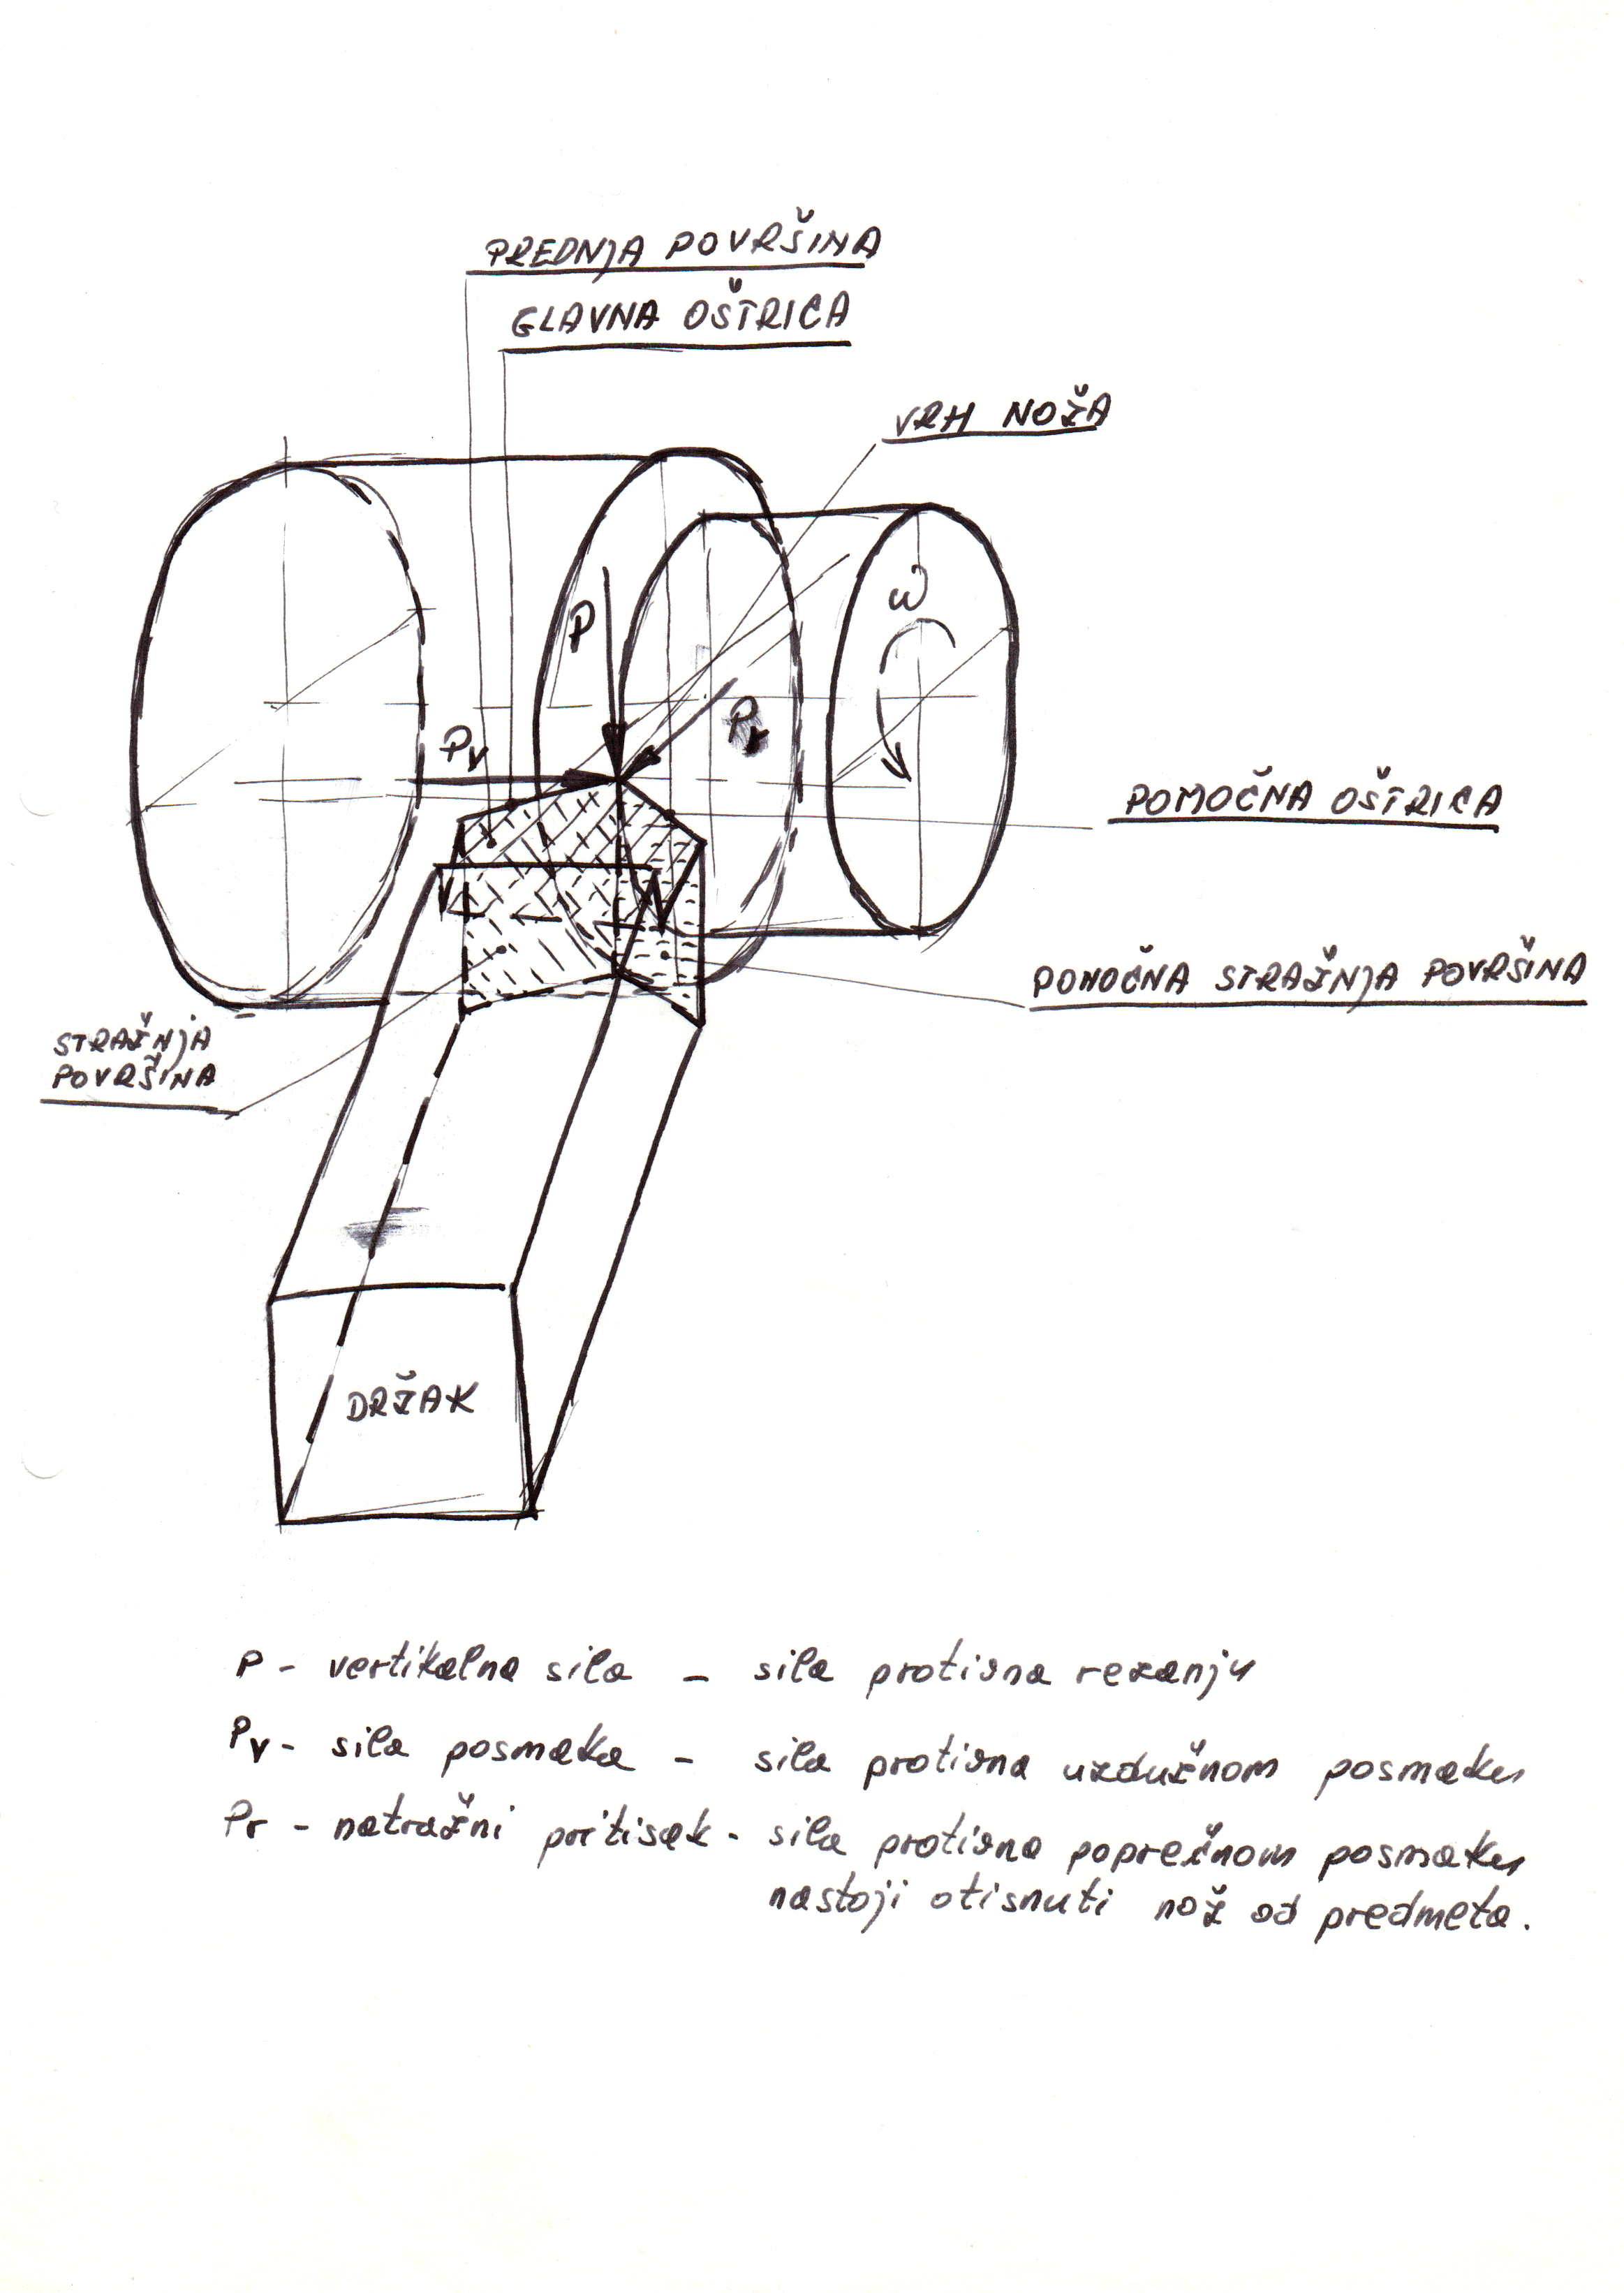
\includegraphics[width=\textwidth]{image_01.png}
\end{figure}
\FloatBarrier
\noindent Osnovni elementi su:
\begin{itemize}
\item glavna oštrica
\item pomoćna oštrica
\item noža.
\end{itemize}
Od površina koje trebamo razlikovati na nožu su
\begin{itemize}
\item prednja površina
\item stražnja površina
\item pomočna stražnja površina.
\end{itemize}
Prije nego što upoznamo detalje noža, spomenimo i sile koje se javljaju na nožu. To su:
\begin{itemize}
\item $\mathsf{P}$ - vertikalna sila- sila protivna rezanju
\item $\mathsf{P_{v}}$ - sila posmaka - sila protivna uzdužnom posmaku
\item $\mathsf{P_{r}}$ - natražni pritisak - sila protivna poprečnom posmaku, a nastoji otisnuti nož od predmeta
\end{itemize}
Sada ćemo se upoznati malo detaljnije s jednim nožem za tokarenje, nožem koji se najčešće koristi.
\begin{figure}[!h]
\centering
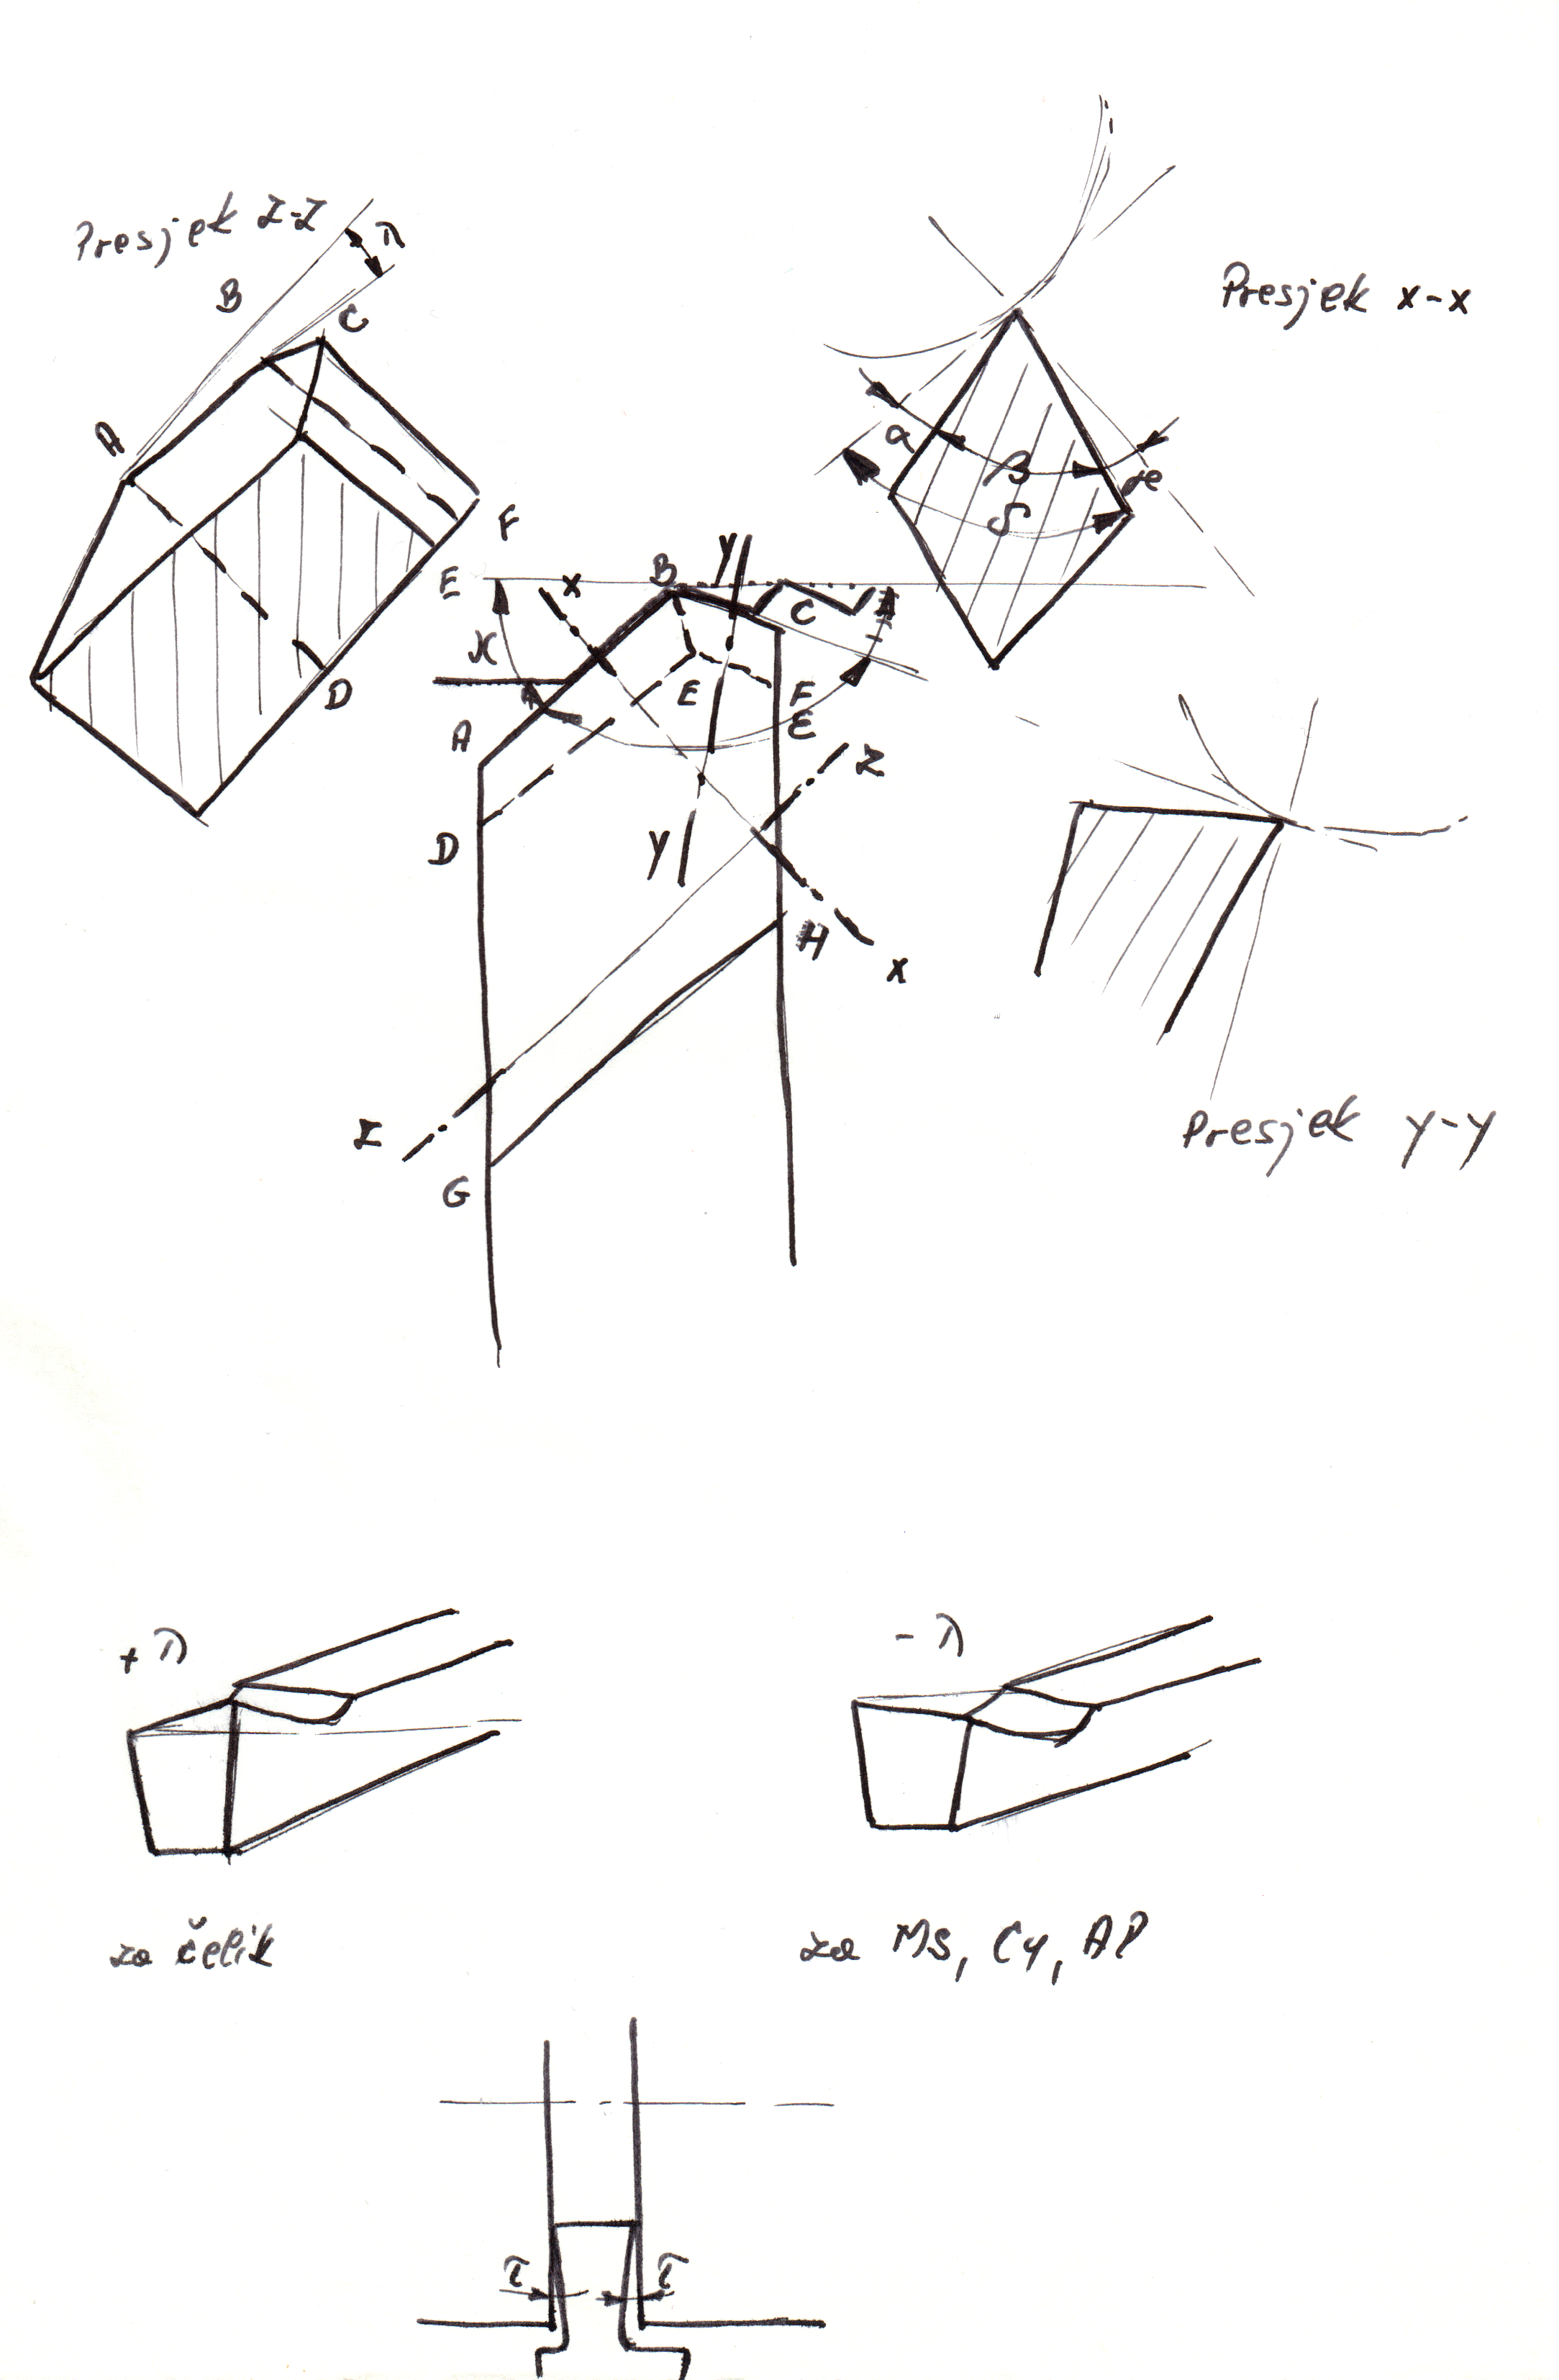
\includegraphics[width=\textwidth]{image_02.png}
\end{figure}
\FloatBarrier
Analizirajući presjek x-x razlikujemo:
\begin{itemize}
\item $\alpha$ - stražnji ili slobodni kut - između stražnje površine i površine rezanja. 
\item $\beta$ - kut oštrenja ili kut klina - kut između prednje i stražnje površine.
\item $\gamma$ - prednji kut, kut između prednje površine i okomice na površinu rezanja. Proizlazi da je $\alpha$ + $\beta$ + $\gamma$ = $90^{\circ}$
\item $\delta$ - kut rezanja - on je suma $\alpha$ + $\beta$.
\item $\epsilon$ - kut šiljka noža ili čeoni kut, to je kut između stražnje i pomočne stražnje površine
\item $\kappa$ - kut namještanja noža je kut između površine rezanja i glavne oštrice
\item $\lambda$ - kut nadvišenja - kut između glavne oštrice i površine u ravnini rezanja koja proizlazi kroz vrh noža
\item $\tau$ - natražni kut - koji se pojavljuje kod noževa za odrezivanje.
\end{itemize}
Evo nekoliko osnovnih primjera brušenja tokarskih noževa.
\begin{figure}[!h]
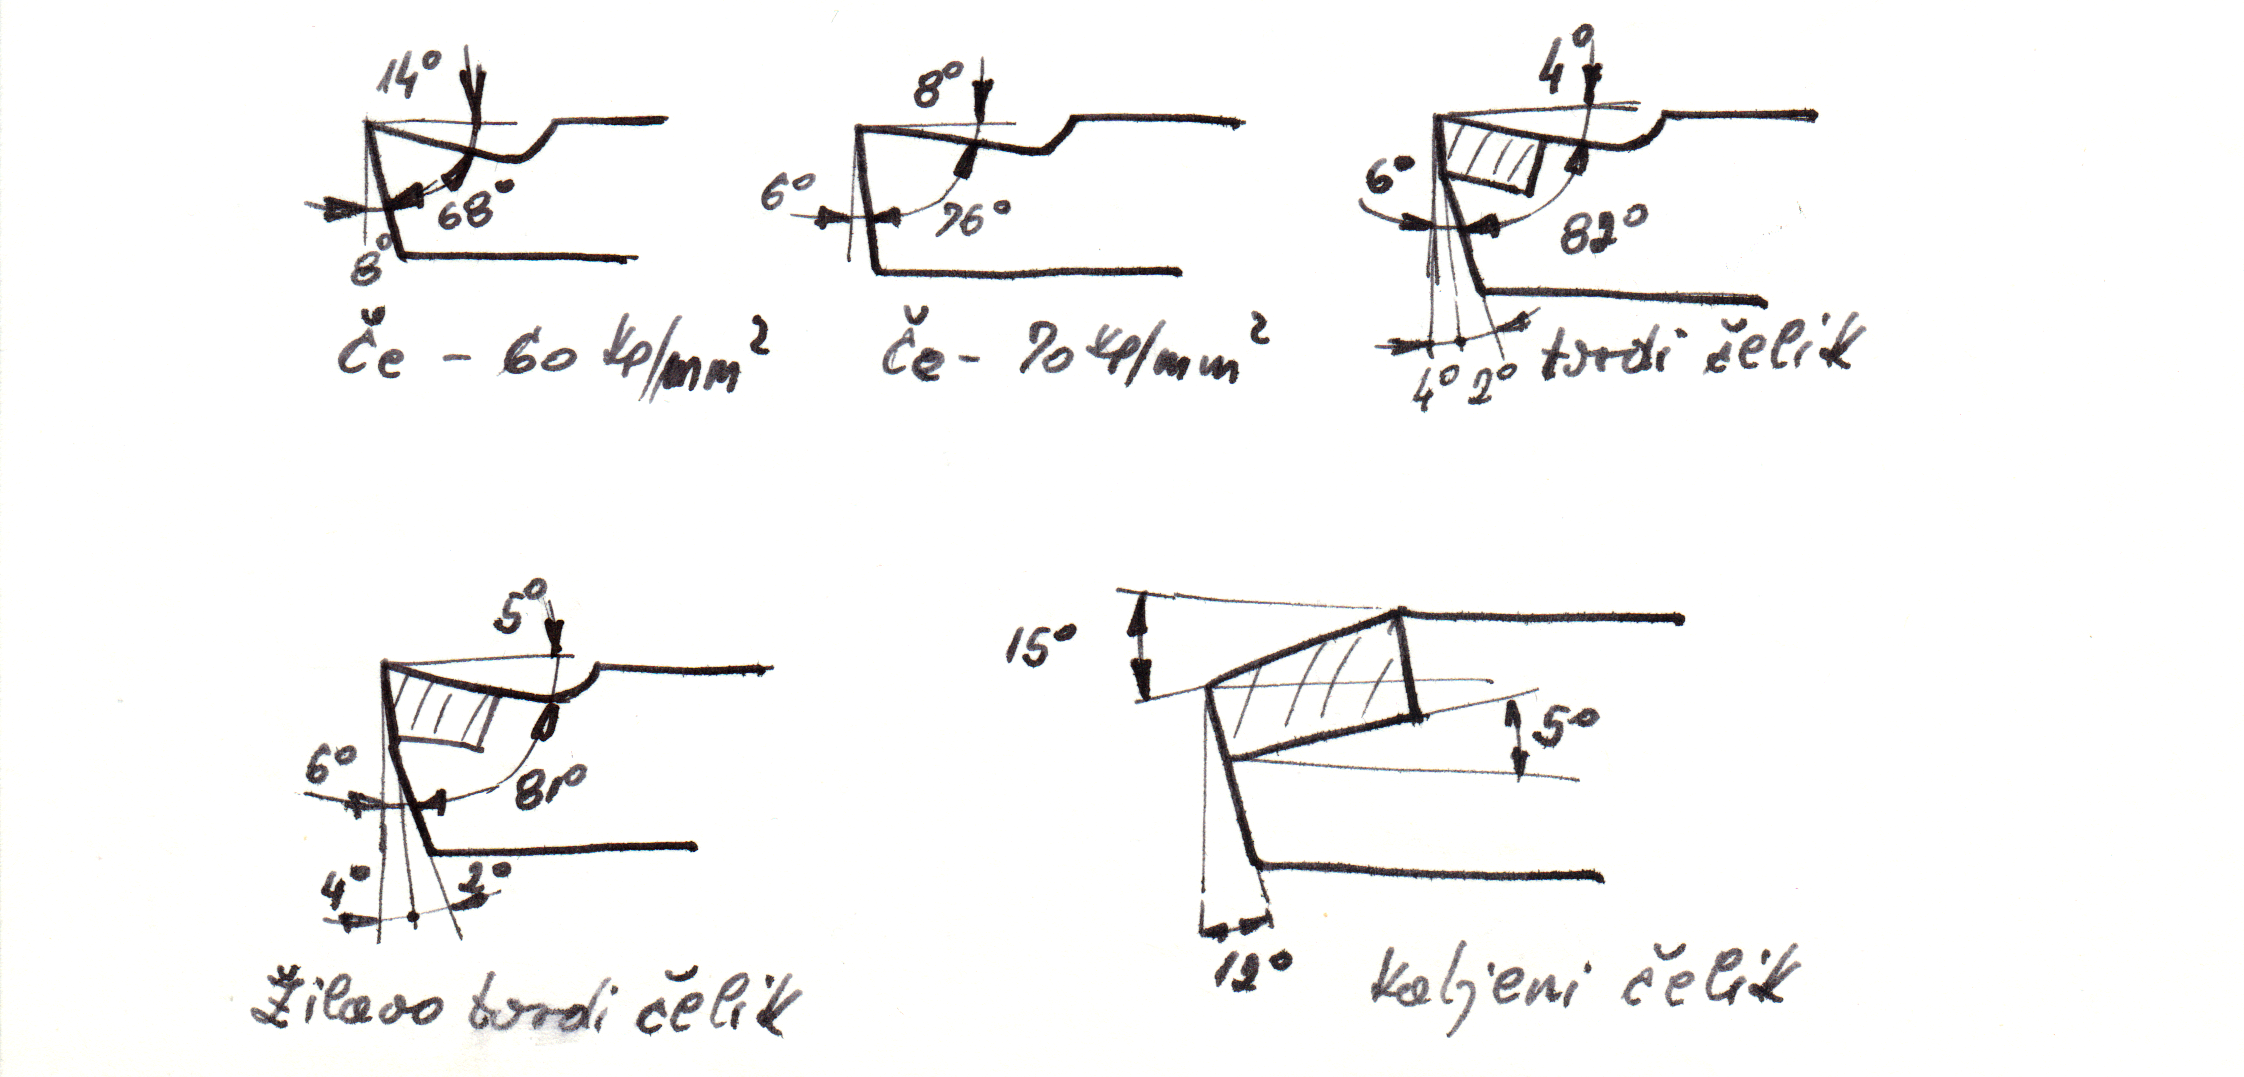
\includegraphics[width=\textwidth]{image_03.png}
\end{figure}
\FloatBarrier
Položaj noža prema tokarenom predmetu može također djelovati na promjene osnovnih kuteva rezanja $\alpha$, $\beta$, $\delta$, dok nam kut $\beta$ ostaje konstantan.
\begin{figure}[!h]
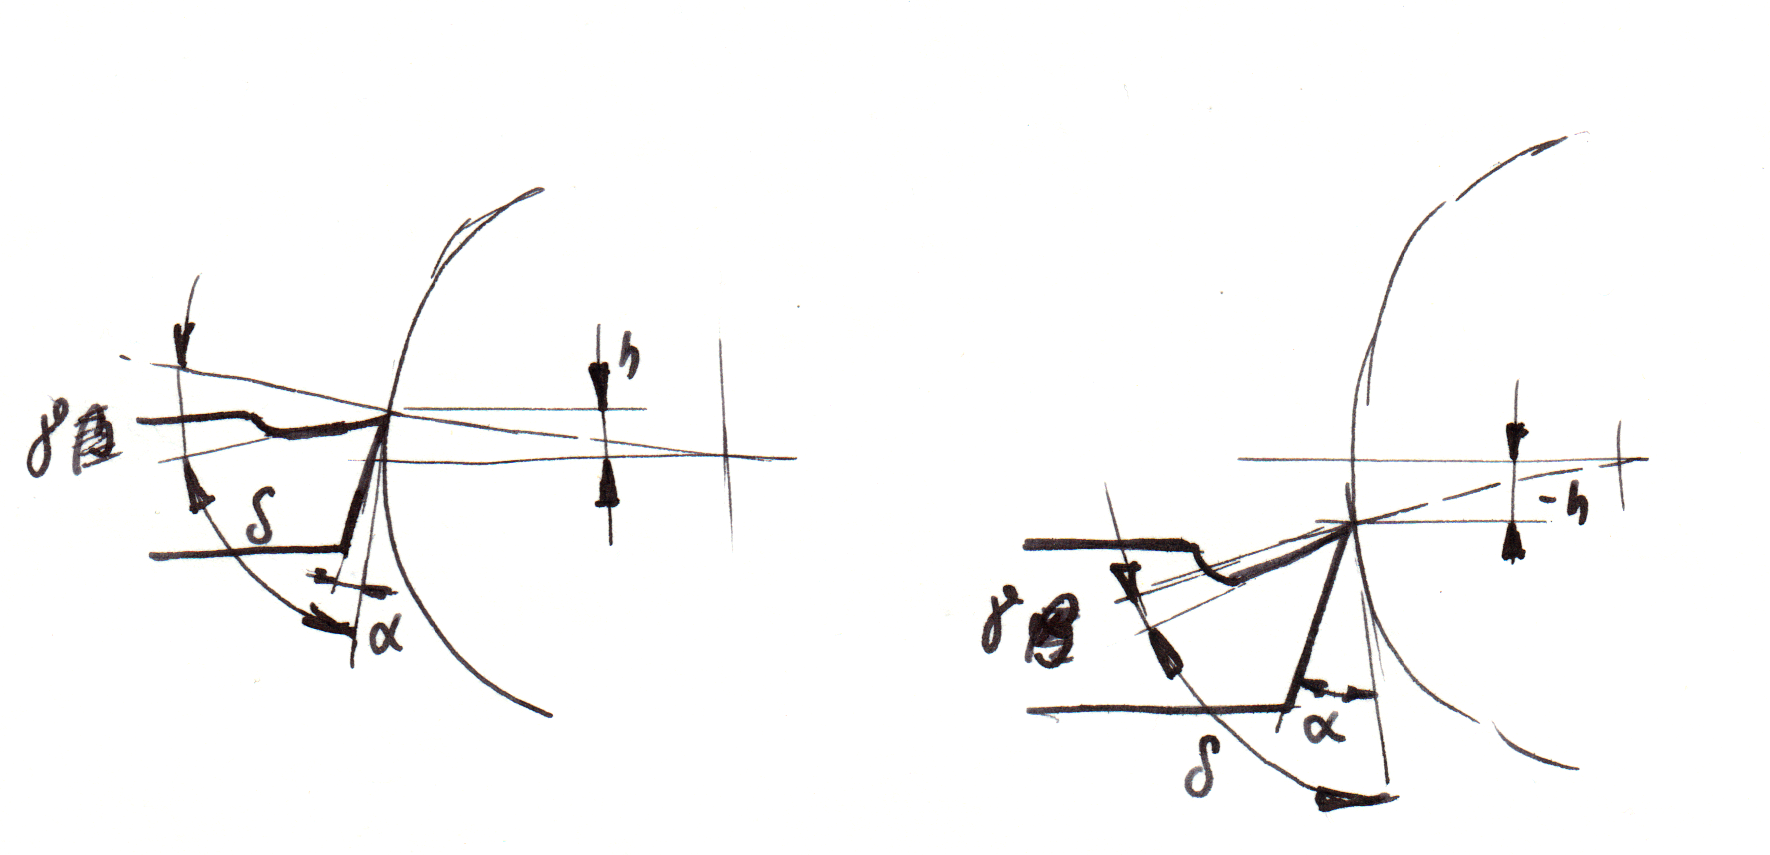
\includegraphics[width=\textwidth]{image_04.png}
\end{figure}
\FloatBarrier
Kod unutarnjeg tokarenja situacija je obratna. To nas upučuje da je važno paziti kako je postavlja nož kod obrade. 
\subsection{Proces rezanja i formiranja strugotine}
Prilikom skidanja strugotine sudjeluje niz faktora koji definiraju oblik strugotine. U te faktore možemo svrstati:
\begin{itemize}
\item vrstu materijala koji se obrađuje
\item vrstu materijala od kojeg je nož
\item brzinu rezanja i 
\item presjek strugotina.
\end{itemize}
Postoje tri osnovna tipa strugotine:
\subsubsection*{Kidane-lomljene strugotine}
\begin{wrapfigure}{l}{0.25\linewidth}
\centering
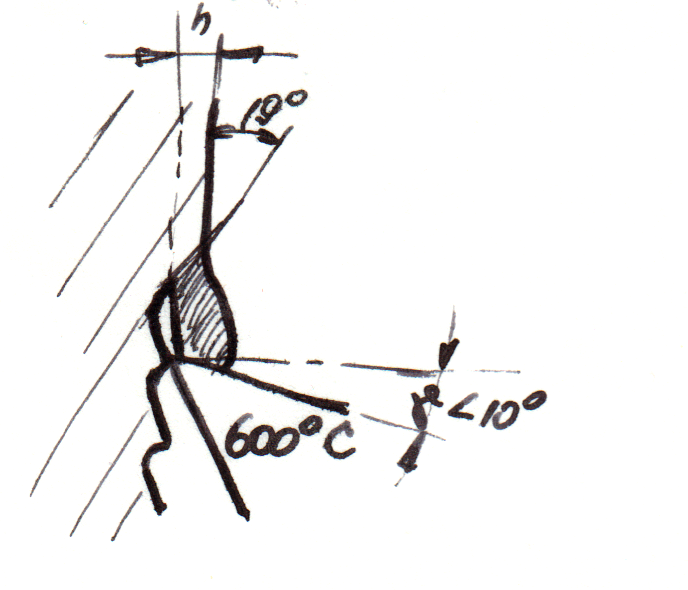
\includegraphics[width=0.25\textwidth]{image_05-1.png}
\end{wrapfigure}
\FloatBarrier
Materijal se najprije sabije na prednjoj površini noža, a zatim se zbog povečanog pritiska odlomi. Nakon toga proces se opet ponavlja.
Kidana - lomljena strugotina nastaje kada je prednji kut manji od $10^{\circ}$, a zatim kod tvrdih materijala i kada se radi s preniskim brzinama rezanja. U tako formiranoj strugotini ne nastaju plastične deformacije. Oštrica noža se grije do $600^{\circ}$C i to nejednoliko. Kako se pritisak mijenja, mijenja se i zagrijavanje oštrice što dovodi do velikog kolebanja temperature. Kod takovog obnlika strugotine podmazivanje noža mnogo ne pomaže. Takav oblik strugotine javlja se kod ljevanog željeza.
\subsubsection*{Rezana ili odrezna strugotina}
\begin{wrapfigure}{l}{0.25\linewidth}
\centering
\vspace{-0.5cm}
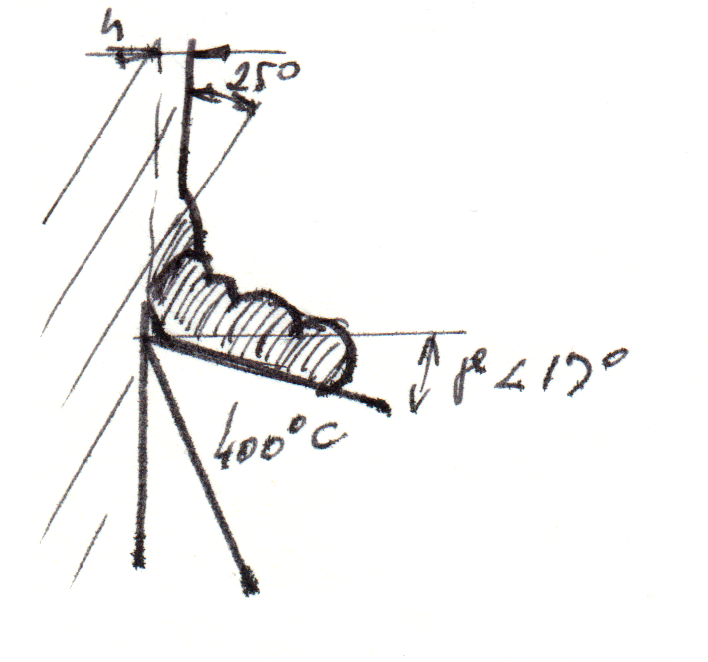
\includegraphics[width=0.25\textwidth]{image_05-2.png}
\vspace{-3cm}
\end{wrapfigure}
\FloatBarrier
Ovakav oblik strugotine nastaje kod prednjeg kuta $\gamma < 17^{\circ}$ i kod male dubine rezanja. Taj oblik strugotine je prijelazni oblik od kidane na trakastu strugotinu. Oblik strugotine je povoljan jer nije preduga i ne smeta pri radu. 

\vspace{1cm}
\subsubsection*{Trakasta ili ljuštena strugotina}
\begin{wrapfigure}{l}{0.25\linewidth}
\centering
\vspace{-0.5cm}
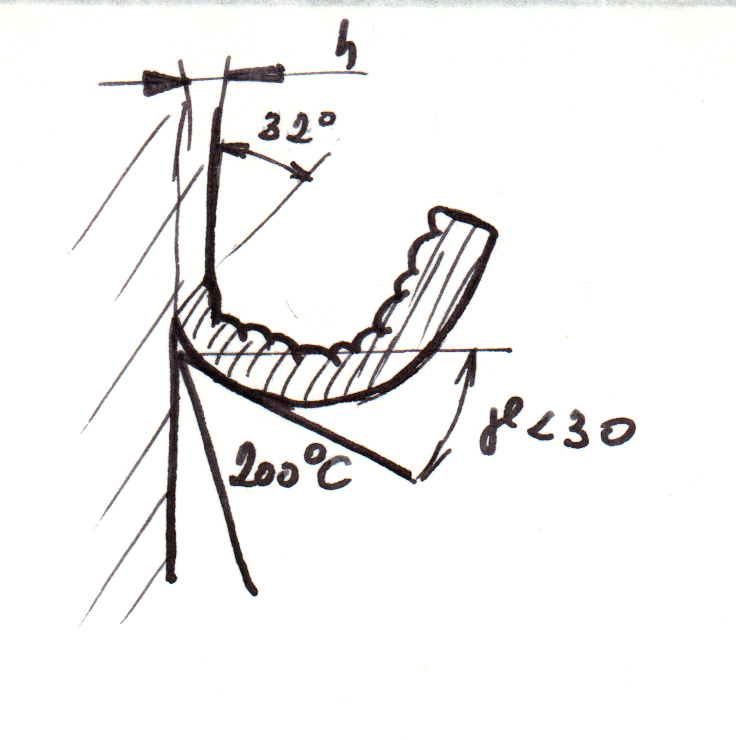
\includegraphics[width=0.25\textwidth]{image_06-1.png}
\end{wrapfigure}
\FloatBarrier
Ovakav oblik strugotine nastaje kod velikih brzina rezanja, male dubine i malog posmaka i kod prednjeg kuta $\gamma<30^{\circ}$. Materijal se tari o prednju površinu noža i odlazi kao neprekinuta strugotina. Pritisak na nož je jednolikiji, što daje i jednoličniju temperaturu oštrice od približno $200^{\circ}$C. Kolebanje temperature noža su u granicama od $20^{\circ}$. Dobrim podmazivanjem oštrice pri rezanju može se produžiti vijek rada noža, jer takovo podmazivanje pogoduje stvaranju povišene oštrice koja štedi oštricu. To svojstvo nam veoma važno kod rada na automatima.
\subsection{Hrapavost obrađene površine}
Kvaliteta obrađene površine ovisi o režimima rada i o izboru noža. Razlikujemo dvije osnovne forme noževa i to:
\begin{itemize}
\item noževi za grubu obradu
\item noževi za finu obradu.
\end{itemize}
Noževi za grubu obradu moraju biti izabrani tako da omoguće maksimalno moguće skidanje strugotina. Sa takovim noževima možemo postići prosječnu hrapavost  $9 - 11\:\mu m$. Noževi za finu obradu već imaju posebne oblike raznih oštrica, te uz dobro izabrane režime rada mogu dati kvalitetu površine od $6-9 \mu m$.
\begin{figure}[!h]
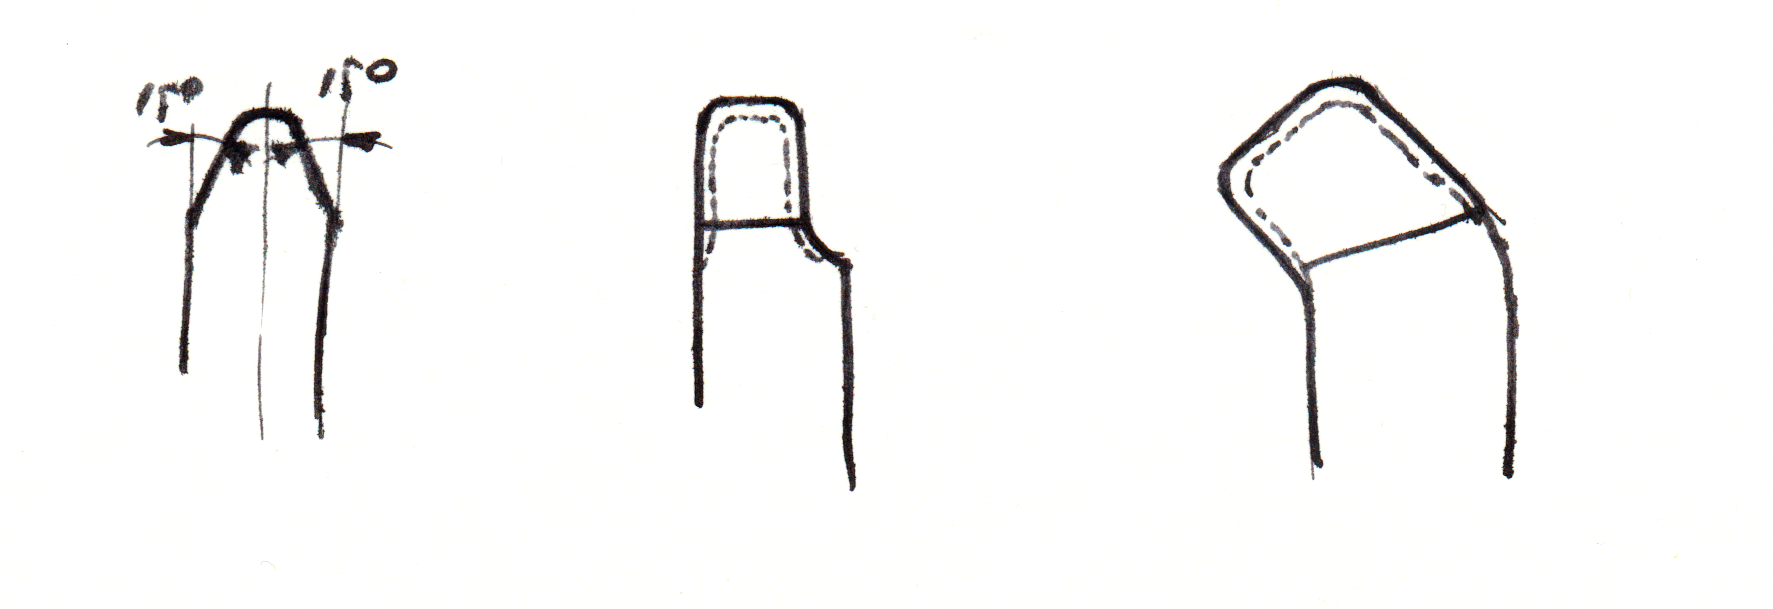
\includegraphics[width=\textwidth]{image_06-2.png}
\end{figure}
\FloatBarrier
Općenito uzevši, tokarski nož za vanjsku obradu možemo prvi moment podijeliti na lijeve i desne noževe. Dali je nož lijevi ili desni oderđujemo na sljedeći način. Uzmemo ga u ruku tako, da oštrica bude okrenuta prema našem tijelu i to prema gore. Strana na kojoj se nalazi glavna rezna oštrica vrijedi kao oznaka (lijevi, desni).\\
Druga podjela noževa za tokarenje može biti:
\begin{itemize}
\item noževi za vanjsko tokarenje
\item noževi za unutarnje tokarenje
\item razni fazonski noževi za vanjsko ili unutarnje tokarenje a tu spadaju i noževi za rezanje raznih vrsta nareza, raznih oblika utora itd.
\end{itemize}
Pregled noževa za vanjsko tokarenje:
\begin{figure}[!h]
\includegraphics[width=\textwidth]{image_07.png}
\end{figure}
\FloatBarrier
\begin{enumerate}
\item - desni savijeni nož za čeono grubo obrađivanje
\item - desni savijeni nož za čeono obrađivanje uglova
\item - desni ravni nož za uzdužno grubo obrađivanje
\item - desni savijeni nož za uzdužno grubo obrađivanje
\item - nož za fino obrađivanje, šiljati
\item - nož za fino obrađivanje
\item - nož za utore
\item - nož za odrezivanje
\item - ravni nož za poprečno tokarenje.
\end{enumerate}
Već smo više puta spominjali termine \textbf{dubina}, \textbf{posmak}, \textbf{presjek strugotine}. Svi ovi termini, veoma se ćesto koriste, kada se govori o skidanju strugotina. Da se sada upoznamo i s tim tako važnim podatcima.
\begin{figure}[!h]
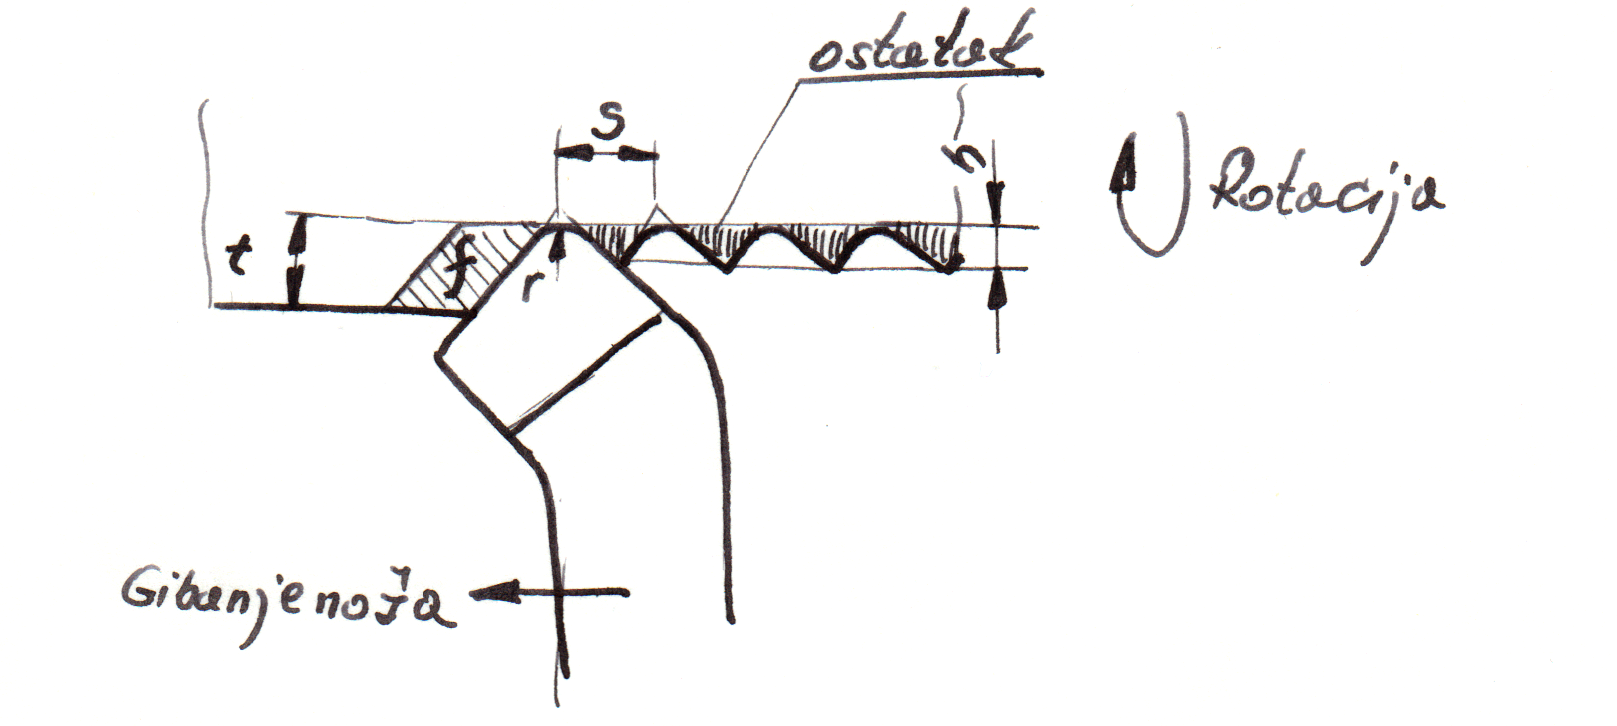
\includegraphics[width=0.7\textwidth]{image_08-1.png}
\end{figure}
\FloatBarrier
\begin{itemize}
\item Dubina rezanja - t - je dubina prodiranja noža u materijal i mjeri se u milimetrima.
\item Posmak noža - s - mm/okretaj - to je pomak noža duž osi obrađivanog predmeta za svaki okretaj.
\item Presjek strugotine - f - mm$^2$ - možemo ga smatrati umnoškom posmaka \textbf{s} i dubine rezanja \textbf{t}; to bi bio teoretski presjek. Stvarni presjek je manji za neskinuti ostatak, koji ovisi o posmaku noža, o kutevima glavne i sporedne oštrice, te o zaobljenosti vrha noža.
\end{itemize}
Analizirajući sliku, veličina neskinutog ostatka naglo raste s porastom posmaka, a isto tako je vidljivo da naglo pada s porastom zaobljenja vrha noža. Jedan od oblika noža koji ostavlja veoma mali ostatak je oblik koji predlaže Taylor. Zbog velike zaobljenosti vrha ostatak je minimalan. No jako zaobljeni noževi imaju cca $15\%$ veće sile rezanja od običnih noževa.
\begin{figure}[!h]
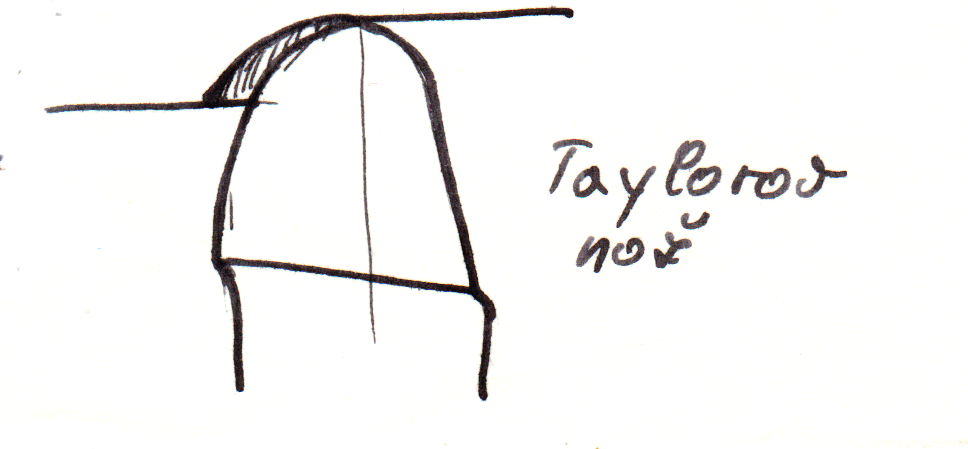
\includegraphics[width=0.5\textwidth]{image_08-2.png}
\end{figure}
\FloatBarrier
\noindent Specifična opterećenja duž ovih oštrica su dosta nejednolika. Zbog takove forme otežana je proizvodnja takovih noževa i međufazno prebrušavanje što dovodi do rijeđe primjene ovakovih oblika noževa. 
\subsubsection*{Sile na nožu}
U početku smo se već upoznali sa silama, koje se javljaju na nožu. Kod toga razlikujemo:
\begin{itemize}
\item $\mathsf{P}$ - vertikalnu silu - silu protivnu rezanju
\item $\mathsf{P_{v}}$ - sila posmaka - sila protivna uzdužnom posmaku
\item $\mathsf{P_{r}}$ - natražni pritisak - sila protivna poprečnom posmaku nastoji otisnuti nož od predmeta.
\end{itemize}
\par
Za nas je najinteresantnija vertikalna sila $\mathsf{P}$, jer je ona znatno veća od drugih dviju sila. Odprilike možemo uzeti da je omjer sila na nožu $\mathsf{P}$ : $\mathsf{P_{v}}$ : $\mathsf{P_{r}}$ = $5$ : $2$ : $1$. Iz toga je vidljivo da nam dimenzioniranje drška noža dovoljno uzeti samo vertikalnu silu $\mathsf{P}$. \par
Na veličinu vertikalne sile djeluju mnogi faktori. Kao najutjecajnije smatramo čvrstoću obrađivanog materijala i presjek strugotine. Povezanost ovih dviju varijabli prikazat ćemo u dijagramu.
\begin{figure}[!h]
\includegraphics[width=0.7\textwidth]{image_09.png}
\end{figure}
\FloatBarrier
Takova zakonitost sile $\mathsf{P}$ navodi nas da ju možemo brzo i jednostavno odrediti formulom:
\begin{equation}
\mathsf{P} = A \cdot f \cdot \sigma_{z}\:.
\end{equation}
Gdje je $A$ faktor proporcionalnosti ovisan o materijalu, $f$ presjek strugotine ($s\cdot t$)  i $\sigma_{z}$ čvrstoća materijala na vlak. \par
Eksperimentalno su dobiveni podatci za faktor proporcionalnosti i on se kreće:
\begin{itemize}
\item A = $2,5 - 3,5$ za čelične materijale
\item A = $4,5 - 5,5$ za lijevano željezo
\item A = $3 - 4$ za Al i Al-legure.
\end{itemize} 
Na veličinu sile rezanja ne utjeće samo čvrstoća materijala i presjek strugotine nego još i
\begin{itemize}
\item oblik presjeka strugotine koju može imati različite omjere posmaka i dubine rezanja, a može i oštrica biti zaobljena pa je presjek skidane strugotine duž oštrice raznolik (Taylorov nož)
\item o kutu klina - oštrenja $\beta$
\item o kutu namještanja noža $\kappa$
\item o brzini rezanja
\item o hlađenju i mazanju - kod lomljene strugotine sistemom mazanja nemožemo smanjiti silu
\item o unutaranjim naprezanjima u materijalu koji obrađujemo.
\end{itemize} 
Snaga potrebna za stvaranje strugotine, troši se najvećim dijelom na rad deformacije strugotine ($75\%$), zatim na rad rezanja ($15\%$) i na rad trenja ($10\%$).
Da bi sve ove faktore uzeli u obzir pri određivanju sile rezanja koristimo se formulom:
\begin{equation}
\mathsf{P} = f \cdot k_{s}\:,
\end{equation}
gdje je $f$ presjek strugotine (mm$^{2}$), a $k_{s}$ koeficijent otpora rezanja (Kp/mm$^{2}$). Koeficijent $K_{s}$ određuje se eksperimentalno ili približno prema nekim formulama.
Za točno definiranje sile rezanja pri nekim uvjetima uz odabrane režime i oblik noža, moguće je jedino saznati kroz eksperimente.
\subsubsection{Radnja rezanja}
Kod uzdužnog tokarenja, od triju sila koje se pojavljuju na nožu potrebno je savladati vertikalnu silu $\mathsf{P}$ i horizontalnu silu posmaka $\mathsf{P_{v}}$. Da bi odredili radnju rezanja uz poznavanje tih sila trebamo znati i brzinu rezanja $v$ i brzinu posmaka $v_{s}$ (m/min). Iz tih podataka dobivamo
\begin{equation}
N_{rez} = \mathsf{P} \cdot \frac{v}{60 \cdot 75} + \mathsf{P_{r}} \cdot \frac{v_{s}}{60 \cdot 75}\:.
\end{equation}
Pošto je $\mathsf{P_{r}}$ 2 do 3 puta manja od $\mathsf{P}$ a $v_{s}$ i preko 100 puta manja od $v$, možemo drugi član ove formule zanemariti, te nam preostaje
\begin{equation}
N_{rez} = \frac{\mathsf{P} \cdot v}{4500}\:.
\end{equation}
Da bio saznali potrebnu snagu za vršenje tokarenja, potrebno je uz radnju savladati i ostale otpore koji se javljau u tokarskom stroju. Mjerenja su pokazala da je ukupna potrebna snaga stroja za $50\%$ veća od radnje rezanja što nam daje 
\begin{equation}
N_{tot} =1.5 \cdot N_{rez} = \frac{\mathsf{P} \cdot v}{3000}\:.
\end{equation}
\subsubsection{Mjerenje sila na noževima}
Prva podjela uređaja kojima mjerimo sile na nožu su na mehaničke uređaje i elektroničke metode. Mehanički uređaji za mjerenje sile sastoje se od ploče, poluge ili pera, na koji djeluje sila. Zbog djelovanja vanjske sile dolazi do elastične deformacije odnosno do pomaka iz nultog položaja. Veličina pomaka mjerimo raznim instrumentima (komparatorima ili manometrima) koji su baždareni da pokazuju veličinu sile.\par
Elektroničke metode registriranja mogu biti ostvarene na više načina:
\begin{enumerate}
\item \textbf{Piezoelektričkim} - prijenos sile kvarcne kristale u kojima se javlja elektrostatski naboj čiju količinu mjerimo. Veličina elektrostatskog naboja proporcionalna je veličini djelujuće sile na kristale.
\item \textbf{Kapacitivnim} - djelovanje vanjske sile izaziva pomake koji se prenose neki elastični ili cilindrični kondenzator. Kondenzator je uključen u krug struje, a njegovom deformacijom mijenja se jakost struje čiju promjenu registrira galvanometar, baždaren u tu svrhu kilogramima.
\item \textbf{Induktivni} - pod djelovanjem vanjske sile dolazi do promjene zračnog raspora a to mijenja jakost inducirane struje u sekundarnoj zavojnici. Mjerenjima te promjene dolazimo do veličine sile koja je izazvala promjenu zračnog raspora.
\item \textbf{Magnetoelastični} - način se temelji na jakom utjecaju mehaničkih sila na krivulju magnetiziranja magnetoelastičnih materijala. Kroz svitak žice teće izmjenična struja, čija jakost ovisi o priključenom naponu, električnom otporu žice a i promjene megnetskih svojstava jezgre djeluju na veličinu struje čije promjene registriramo na instrumentima.
\begin{figure}[!h]
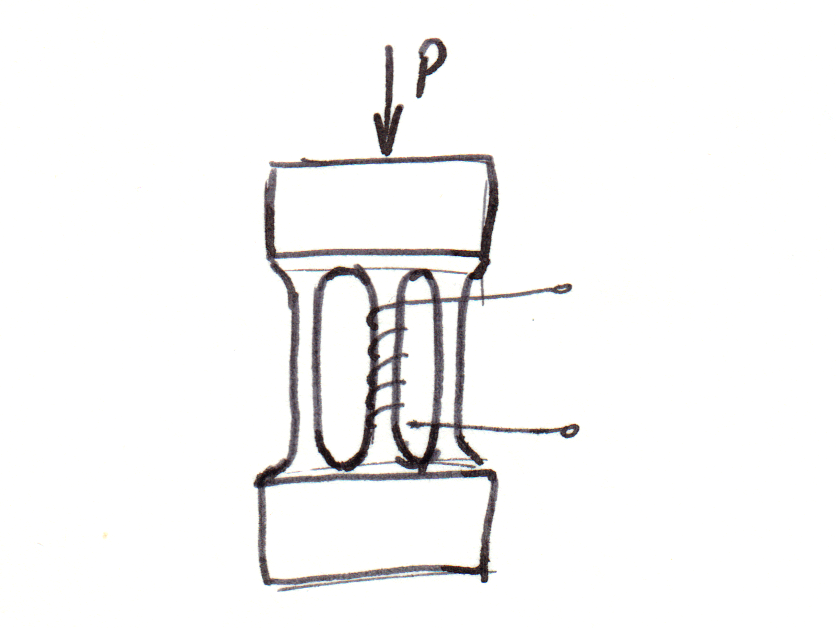
\includegraphics[scale=0.2]{image_10-1.png}
\end{figure}
\FloatBarrier
\item \textbf{Elektrolitički način} - električna vodljivost nekog elektrolita ovisi o specifičnom otporu samog elektrolita i o presjeku sloja elektrolita kroz koji prolazi struja. Vanjska sila mijenja presjek sloja, vodljivog elektrolita a time povećava njegov otpor koja protiće elektrolitom. Ampermetar registrira promjenu jakosti struje koja je neka funkcija sile.
\item \textbf{Elektrootporni način} - iz fine žice velikog otpora ($100 - 1000\:\ohm$) napravljene su mjerne trake. Ljepljenjem tih traka na mjesta koja će preživjeti deformacije zbog djelovanja vanjskih sila moći ćemo saznati veličinu sile mjereći promjene jakosti struje koja protiće kroz mjernu traku.
\begin{figure}[!h]
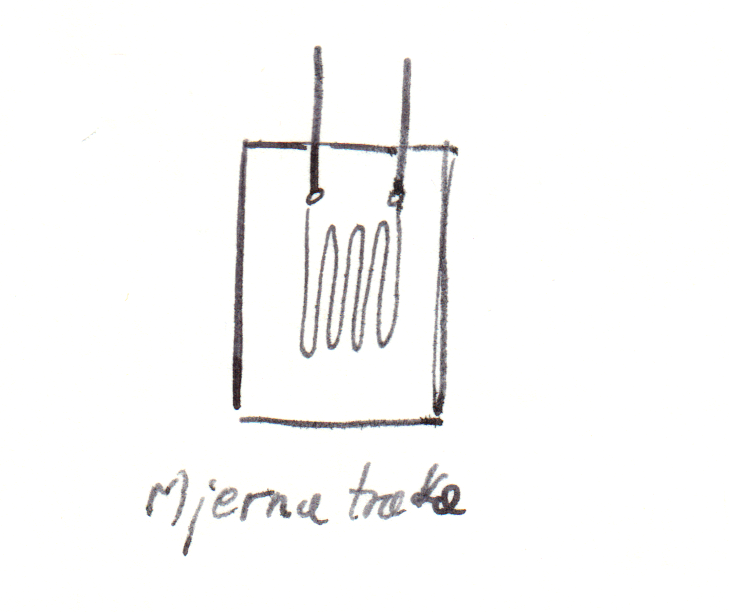
\includegraphics[scale=0.2]{image_10-2.png}
\end{figure}
\FloatBarrier
Zbog deformacija predmeta na koje su zaljepljene mjerne trake deformirat će se žica u mjernim trakama, što opet izaziva promjenu otpora žice koju registrira instrument. 
\end{enumerate}
Danas u principu najviše koriste metode električnog mjerenja jer imaju niz  prednosti a najvažnija je jednostavnost.
\subsection{Toplina pri procesu rezanja}
Nastanak topline pri procesu skidanja strugotine je višestruka:
\begin{enumerate}
\item \textbf{Mehanički rad} - pretvara se djelomično u toplinu zbog međusobnog trenja čestica strugotina, kod formiranja strugotine i zbog kidanja strugotine.
\item \textbf{Toplina koja se stvara zbog trenja strugotine o oštricu noža} - proizvedena toplina ovisi o 
\begin{itemize}
\item brzini rezanja
\item debljini strugotine
\item materijala koji se obrađuje.
\end{itemize}
\begin{figure}[!h]
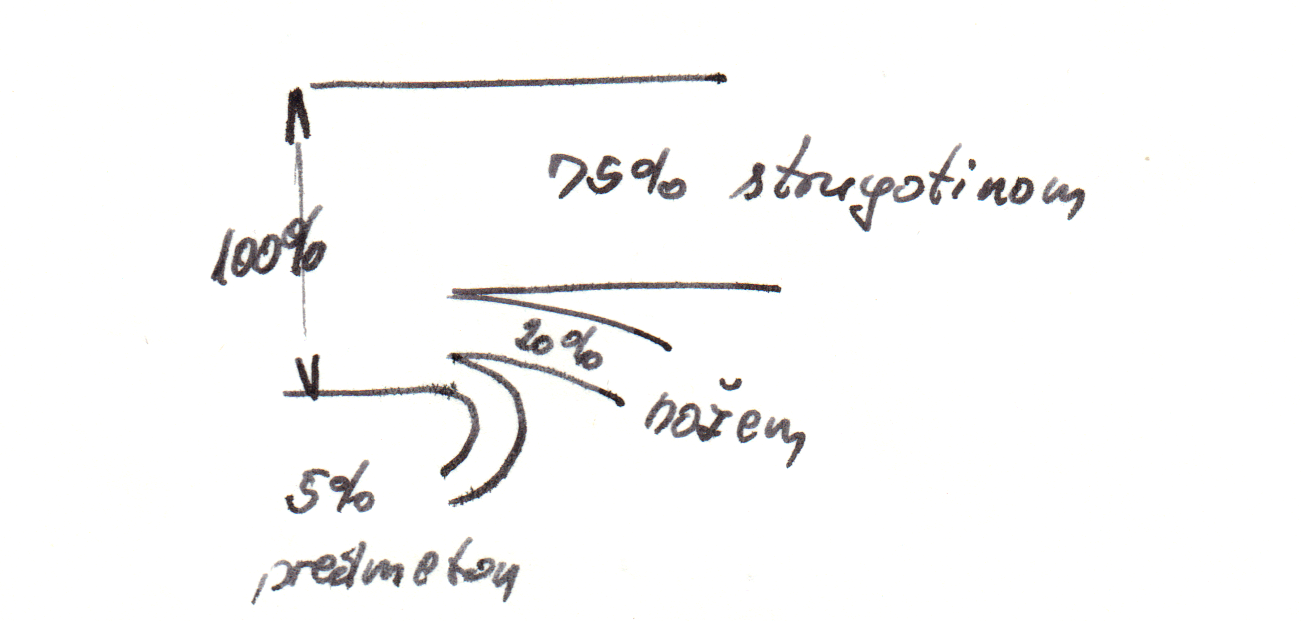
\includegraphics[width=0.7\textwidth]{image_11-1.png}
\end{figure}
\FloatBarrier
\item \textbf{Strugotina odvodi} sa sobom količinu topline koja proporcionalna presjeku strugotine. Jasno da tu vezano odvođenje topline i s brzinom rezanja.
\item \textbf{Nož odvodi} u principu uvijek iztu količinu topline, i ima zbog svojih dimenzija, konstantni toplinski kapacitet.
\item \textbf{Obrađeni predmet} se zbog preuzetog dijela topline obično rastegne, odnsono promjeni svoje dimenzije. Zbog toga se predmet mora mjeriti na temperaturi okoline.
\end{enumerate}
Toplina koja se prenosi na nož i diže temperaturu noža nepovoljno nam djeluje na izdržljivost oštrice.
\begin{wrapfigure}{l}{0.3\textwidth}
\vspace{-0.5cm}
  \begin{center}
    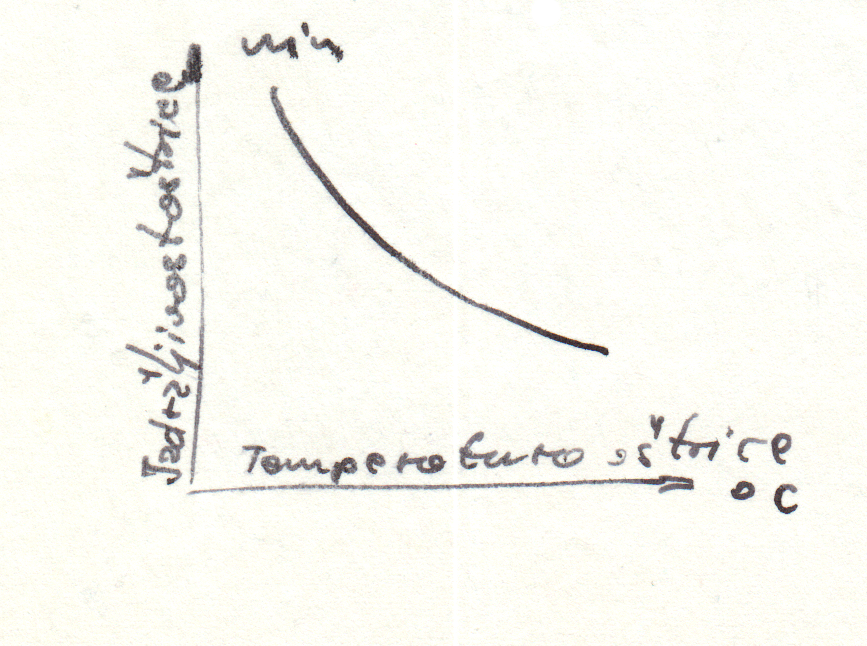
\includegraphics[width=0.3\textwidth]{image_11-2.png}
  \end{center}
  \vspace{-1cm}
\end{wrapfigure}
Iz dijagrama je vidljivo da je izdržljivost oštrice, tj. vrijeme rezanja u minutama, manje čim je temperature oštrice veća.\par 
Za razne tipovealatnih strojeva, poželjno nam je da nam neki nož izdrži određeno vrijeme rada s nekim optimalnim režimima. Ti zahtjevi su inicirali najrazličitije zahvate za pronalaženje materijala koji će moći izdržati sve teže režime rada. to je dovelo do odkrivanja materijala koji posjeduju velike mogužnosti i kod vrlo visokih temperatura. Tako možemo ukratko reći da su najpoznatiji materijali iz kojih se rade alati za skidanje strugotina:
\begin{figure}[!h]
\centering
\includegraphics[width=0.8\textwidth]{image_12.png}
\end{figure}
\FloatBarrier
\begin{enumerate}
\item \textbf{Alatni čelici} - osnovna im je karakteristika da u sebi imaju $1-1,45\%$ ugljika kad se na $700 - 850^{\circ}$C a napuštaju kad dođu na $180 - 250^{\circ}$C. Noževi od alatnog čelika se lako i dobro obrađuju a daje da su jeftiniji.
\item \textbf{Brzorezni čelici} - su legirani čelici koji u sebi sadrže volframa (W), kroma (Cr), vanadija (V) i molibdena (Mo). Kod kaljena prvo se polagano grije do crvenog žara a onda naglo do $1250 - 1350^{\circ}$C. Napušta se na temperaturu $200 - 270^{\circ}$C ili $575 - 600^{\circ}$C što ovisi o postotcima legiranih elemenata.
\item \textbf{Stelit} - je u stvarnosti tvrđa slitina koja omogućava korištenje još većih brzina rezanja od brzoreznih čelika. Stelit ima približno sastav od $40-50\%$ Co, $25 - 35\%$ Cr, $12 - 20\%$ W, $0,5-3\%$ C.
\item \textbf{Widia} - (wie Diamant) - materijal koji omogučava daljnje povečanje režima rada na alatnim strojevima. Za razliku od stelita koji se dobiva ljevanjem, widia se dobiva tako da se prašak volframova titana i molibdena s nekim vezivnim sredstvom (običnom kobaltom ili niklom) veže. Takvoj smjesi se prešanjem daje određeni oblik i zatim se peće. Jedno pećenje je na $1400^{\circ}$C a drugo na $1900^{\circ}$C. Obrađivati pločice možemo jedino brušenjem.
\item \textbf{Dijamanti} - noževi napravljeni od dijamanata su noževi koji omogućavaju maksimalne režime rada. Korištenje dijamantnih noževa je opravdano kod fine obrade slitina, papira, gume, umjetinih masa bronce i mesinga. Ne isplati se koristiti za nekaljene čelike. Možemo približno uzeti da je odnos cijena između brzorezanog čelika, trvde slitine i dijamanta 1 : 5 :150. Omjer brzine rezanja je 1 : 6: 10, a dozvoljene temperature rezanja 1 : 1,35 : 3.\par
Na kraju izlaganja o temperaturama kod skidanja strugotina moramo još spomenuti da postoji čitav niz rashladnih sustava koja jednom odvode dio topline a kroz to omogučavaju povećanje režima rada. Uz odvođenje topline rashladno sredstvo omogučava dobivanje glatke površine nakon obrade, pospješuje odvođenje strugotine. Kao najpoznatije rashladno sredstvo je \textbf{emulzija} mlječna otopina sapuna i mineralnog ulja. Osim toga koriste se razne vrste ulja koja smanjuju trenje, dok se kod obrade ljevanog željeza za hlađenje noža koristi komprimirani zrak koji ujedno odpuhuje lomljenu strugotinu.
\end{enumerate}
\subsection{Ekonomske brzine rezanja}
Kod skidanja strugotina poželjno nam je da nam brzina rezanja bude što veća, jer nam to omogućava produktivniju proizvodnju a kroz to i ekonomičniju proizvodnju. Velike brzine rezanja, izazivaju brže zatupljenje noža, pa je potrebno češće prebrušavanje i ponovno namještanje noža. \par
Povezanost troškova obrade i troškova namještanje alata u ovisnosti brzine rezanja možemo prikazati u dijagramu.
\begin{figure}[!h]
\centering
\includegraphics[width=0.8\textwidth]{image_13.png}
\end{figure}
\FloatBarrier
Iz dijagrama je vidljivo da postoji samo jedna ekonomska brzina rezanja za neki alat. Tako se za to koriste noževi od brzorezanog čelika. Ekonomska brzina smatra onu brzinu rezanja kod koje alat između dva prebrušavanja izdrži 60 okr/min, a označava se s $^{\nu}$60.\par 
Za složenije alate, za koje je vrijeme prebrušavanja znatno veće a često prebrušavanje smanjuje vijek trajanja alata odabiru se kao ekonomske brzine $^{\nu}$240 i $^{\nu}$480. U tu grupu alata ulaze fazonski noževi, glodala i drugi. \par
I kod jednostavnijih alata koji se doduše brzo prebrušavaju, ali je njegovo namještanje skopčano s većim gubitkom vremena oko ponovnog namještanja na stroj, često se koriste brzine $^{\nu}$480. To se odnosi na alate koji se koriste na automatskim strojevima. \par
Kod svrdala se ekonomskom brzinom smatra ona brzina, kod koje svrdlo može izbušiti ukupno 2000 mm rupa. Ta se brzina označava s $^{\nu_{l}}$2000.
\section{Blanjanje i dubljenje}
Blanjanje je obrada predmeta skidanjem strugotina s jednim nožem. Međusobno pomicanje noža i predmeta je po pravcu. Kod toga razlikujemo dvije mogučnosti međusobnog gibanja noža i predmeta:\\
\begin{wrapfigure}{l}{0.25\textwidth}
  \begin{center}
  \vspace{-1cm}
    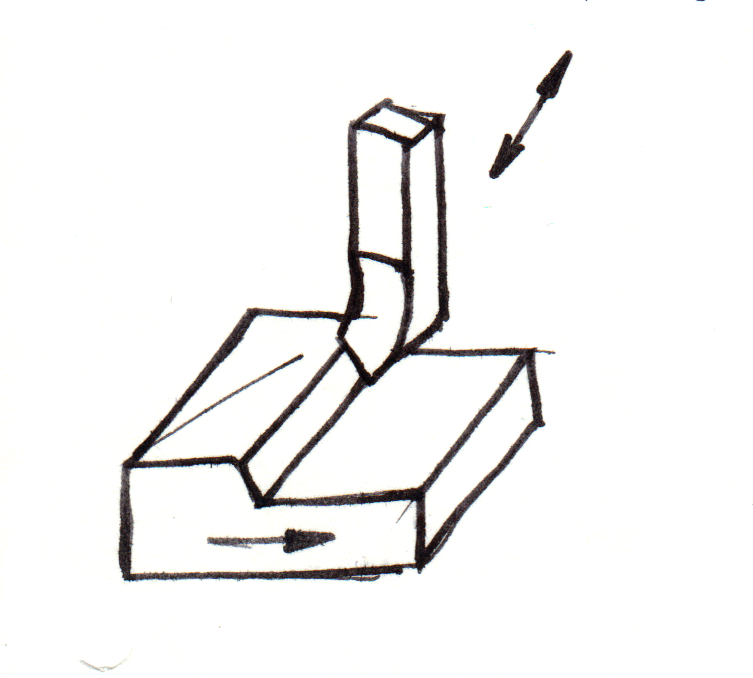
\includegraphics[width=0.2\textwidth]{image_14-1.png}
  \end{center}
\end{wrapfigure}
\begin{wrapfigure}{r}{0.25\textwidth}
\vspace{-3cm}
  \begin{center}
    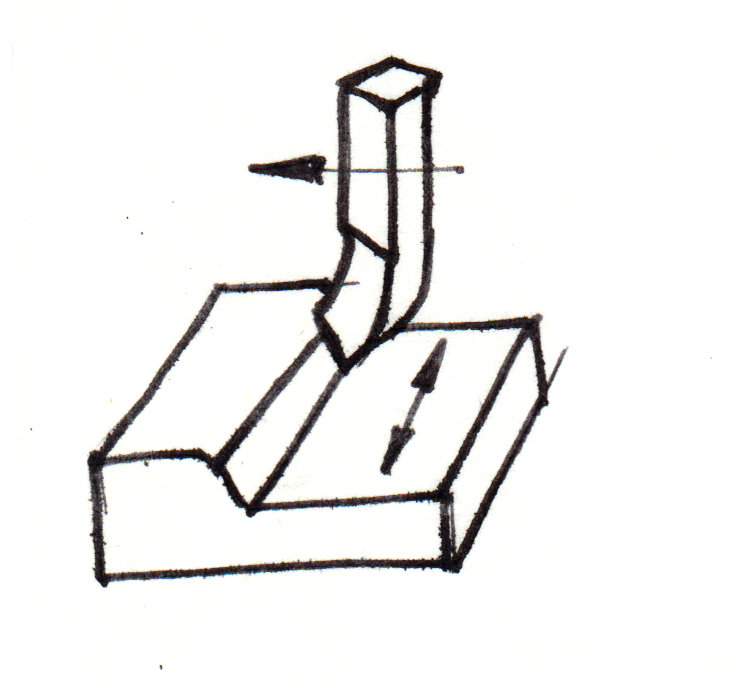
\includegraphics[width=0.2\textwidth]{image_14-2.png}
  \end{center}
\end{wrapfigure}
1. Nož vrši glavno kretanje a predmet vrši posmak. Takav način rada primjenjuje se kod kratkohodnih blanjalica ili šepinga. Maksimalna dužina hoda noža je fo 700 mm.\\
2. Predmet vrši glavno kretanje a nož vrši posmak. Predmet je učvršćen na stolu koji se gibapo saonicama, a nož je učvršćen na zasebnoj gredi po kojoj ostvarije posmak. Takav naćin međusobnog gibanja noža i predmeta primjenjuje se kod dugohodnih blanjalica, a točnost obrade je bolje nego kod kratkohodnih blanjalica.\par
\vspace{2cm}
\noindent Kod glavnog kretanja blanjalica razlikujemo:
\begin{itemize}
\item Radni hod - kada nož skida strugotinu
\item Jalovi hod - kada se nož vrača
\end{itemize}
U grupu blanjlica spada i vertikalna blanjalica, od koje je gibanje noža vertikalno i to
\begin{itemize}
\item odozgo na dolje - glavno kretanje - radni hod
\item odozdo na gore - glavno kretanje - jalovi hod
\item posmak stola može biti u ravnini ili po luku.
\end{itemize}
Postoje i specijalne vrste blanjalica za izradu zupčanika. Kao najpoznatije tehnologije blanjalica zupčanika su:
\begin{itemize}
\item FELLOW postupak - gdje je alat u obliku zupčanika.
\item Maagov postupak - gdje je alat u obliku zubne letve.
\end{itemize}
\subsection{Kratkohodna blanjalica - šeping}
Jedan od klasičnih strojeva za obradu malih predmeta, koji ne traže naročito kvalitetne površine je šeping. Razlikujemo dvije vrste pogonskih uređaja za ostvarivanje glavnog kretanja pri šepingu i to:
\begin{itemize}
\item pogon na ekscentar
\item hidraulički pogon.
\end{itemize}
Princip rada šepinga s pogonom na ekscentar. Pogon je  ostvaren preko elektromotora, remenice i zupčanika do kulisnog mehanizma. Na tom mehanizmu možemo ostvariti veči ili manji ekscentritet kulisnog kamena. Na taj način dobivamo veći ili kraći pomak glave na koju je učvršćen nož. Područje pomicanja glave može se posebno regulirati. Posmak predmeta je osiguran preko drugog kulisnog mehanizma koji je povezan s glavnim.
\begin{figure}[!h]
\centering
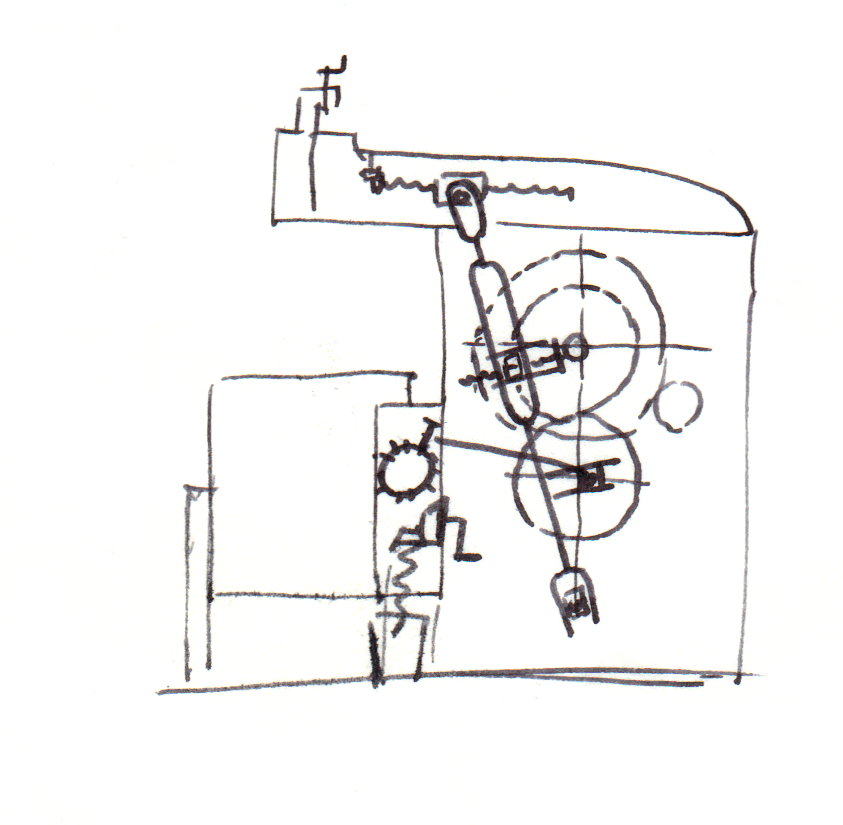
\includegraphics[scale=0.15]{image_15-1.png}
\end{figure}
\FloatBarrier
Nosač noža može ostvariti vertikalno ručno pomicanje, a može se i nagnuti pod izvjesnim kutom za obradu kosina. Radni stol, na kome je smješten predmet može se pomicati ne samo horizontalno, kao nastajanje posmaka, nego i vertikalno pomoću zupčastog prijenosa. Zbog svojeg tereta stol se obično ukruti posebnim podpornjem. 
\begin{figure}[!h]
\centering
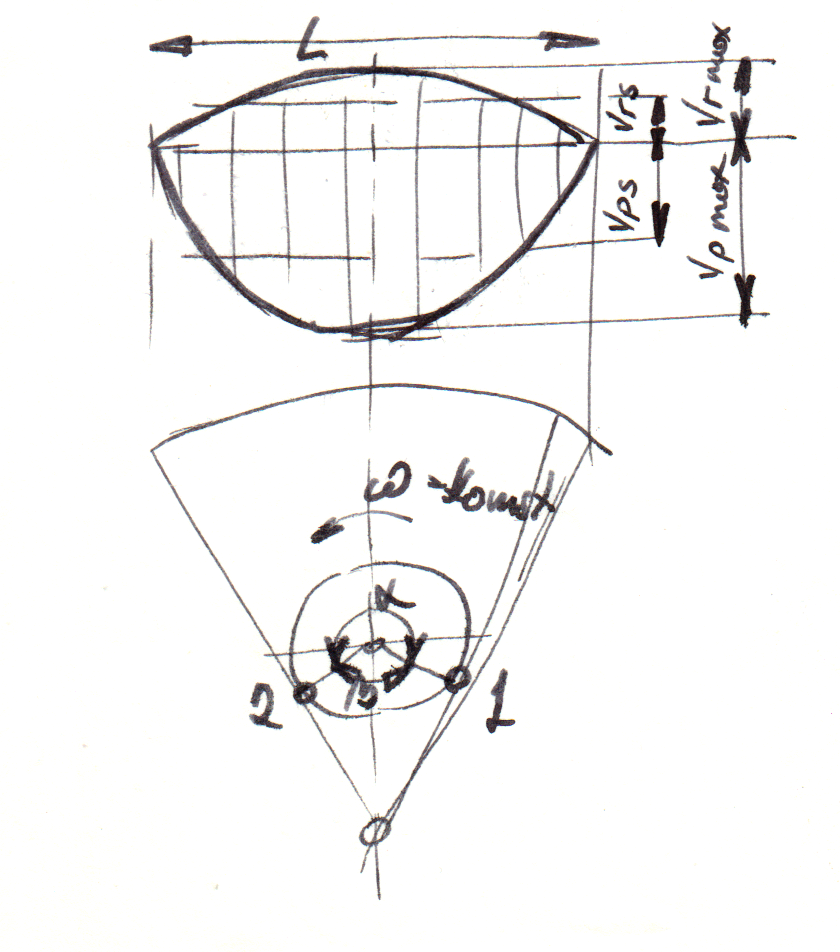
\includegraphics[scale=0.12]{image_15-2.png}
\end{figure}
\FloatBarrier
Dijagram brzina kod kulisnog mehanizma izgleda ovako. Kulisa se kreće od jedne tangente na kružnicu do druge i onda nazad. Na taj način ostvaruje dužina hoda L. Zbog konstantne kutne brzine $\omega$, brzine gibanja glave šepinga od 1 prema 2 po kutu $\alpha$ raste od 0 do $Vr_{max}$. Dok na povratku od 2 na 1 po kutu $\beta$ raste do $Vp_{max}$ i onda pada na nulu. Zbog konstantne kutne brzine i zbog raznolikosti kuteva $\alpha$ i $\beta$ vrijedi odnos:
\begin{equation}
\frac{\mathsf{tr(vrijeme rad.\:hoda)}}{\mathsf{tp(vrijeme par.\:hoda)}} = \frac{V_{ps}}{V_{rs}} = \frac{\alpha}{\beta}>1
\end{equation}
Iz tih podataka, uz poznavanje broja okretaja kulise i dužine puta možemo odrediti brzine rezanja. Stalna promjena brzine rezanja nepovoljno djeluje na kvalitet obrađene površine i na sile na nožu, gdje se javljaju udarci. Da bi se izbjeglo to stalno mijenjanje brzine kod pomicanja noža konstatuirane su blanjalice na hidraulički pogon, kod kojih je brzina radnog ili povratnog hoda, duž čitave radne dužine jednaka. (HRIBAR - 168 strana)
\subsection{Dugohodne blanjalice}
Kod dugohodnih blanjalica, brzina vraćanja radnog stola je  za $2 -3,5$ puta veća od radne brzine. Dugohodne blanjalice mogu raditi i s više od jednog noža što ovisi o veličini blanjalice. Kretanje radnog stola ostvarljivo je ili mehanički preko sistema zupčanika ili hidraulički. Kod manjih dugohodnih blanjalica pogon za automatski posmak noža preuzima se od glavnog pogonskog motora, dok kod velikih dugohodnih blanjalica automatski posmatk noža ima svoj zaseban prigon. Učvršćenje alata izvodi se na glavi predviđenoj za tu svrhu.
\begin{figure}[!h]
\centering
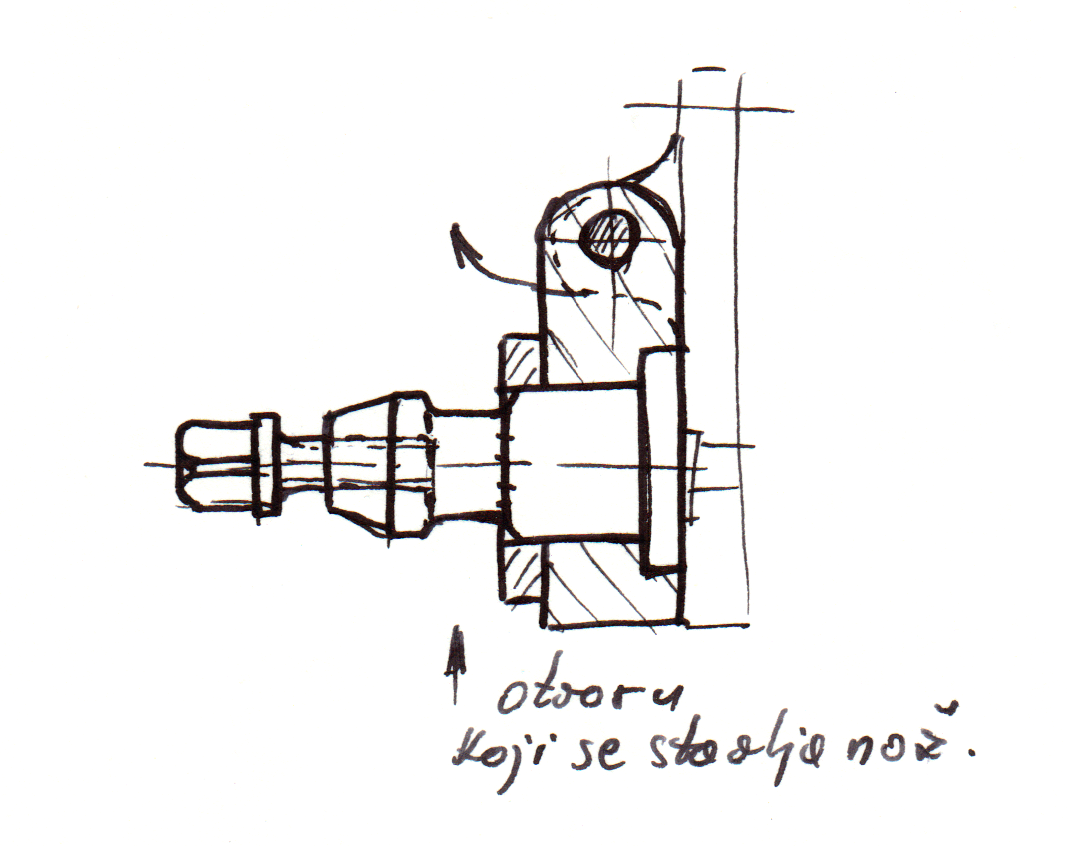
\includegraphics[scale=0.15]{image_16-1.png}
\end{figure}
\FloatBarrier
Specifičnost ovog načina stezanja noža je u tome što glava omogučava podizanje noža od površine pri povratnom hodu. To odmicanje je potrebno, da nož ne zapne za obrađenu površinu i ne ošteti se.\par 
Ako za rad na blanjalici koristimo nož za tokarenje, djelovanje sila na nožu mogu izazvati nepoželjnu deformaciju noža koja može imati višestruke posljedice. \par
Nož upet na ovaj naćin, pod djelovanjem sile rezanja opterećenje je na savijanje. Točka oko koje se javlja moment savijanja je nula. Zbog djelovanja tog momenta, nož će preživjeti izvjesnu elastičnu deformaciju, što izaziva vertikalni pomak oštrice prema dolje za visinu e. Zbog nehomogenosti alata, veličina sile (momenta) se mijenja, usljed čega se mijenja i "e" a kroz to dobivamo lošu površinu i velika je vjerojatnost da će nam vrh noža puknuti. Zbog toga su noževi za blanjanje posebnog oblika, da bi se izbjegle što je moguće više te neugodnosti. Noževi za blanjanje su zbog toga savinuti.
\begin{figure}[!h]
\centering
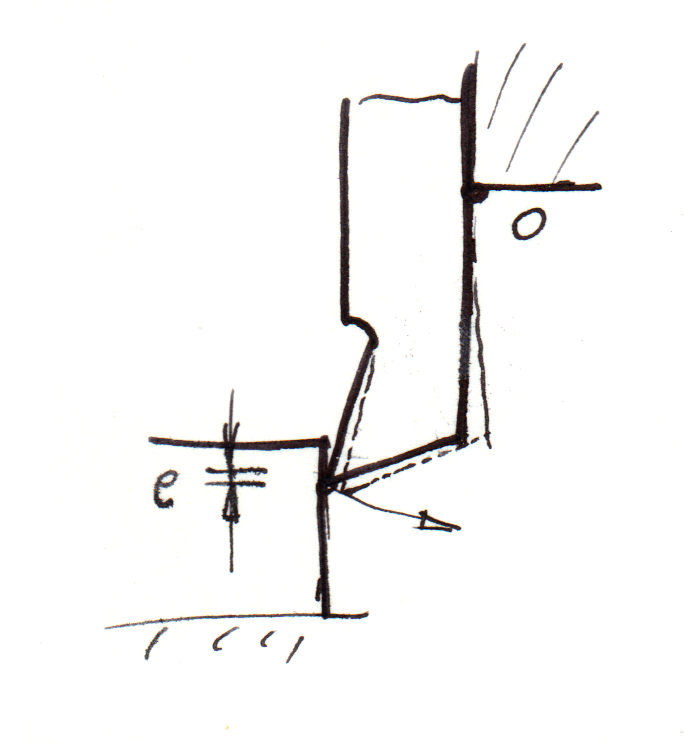
\includegraphics[scale=0.15]{image_16-2.png}
\end{figure}
\FloatBarrier
Kod noževa za blanjanje razlikujemo:
\begin{itemize}
\item noževe za grubu obradu
\item noževi za finu obradu
\item noževi za prostornu obradu.
\end{itemize}
Za učvršćenje noževa postoje i posebne glave koje omogučavaju stezanje noževa i pod kutem. Za blanjanje se koriste i fazonski noževi za obradu np.: utora, vanjskih zakrivljenja itd.
\begin{figure}[!h]
\centering
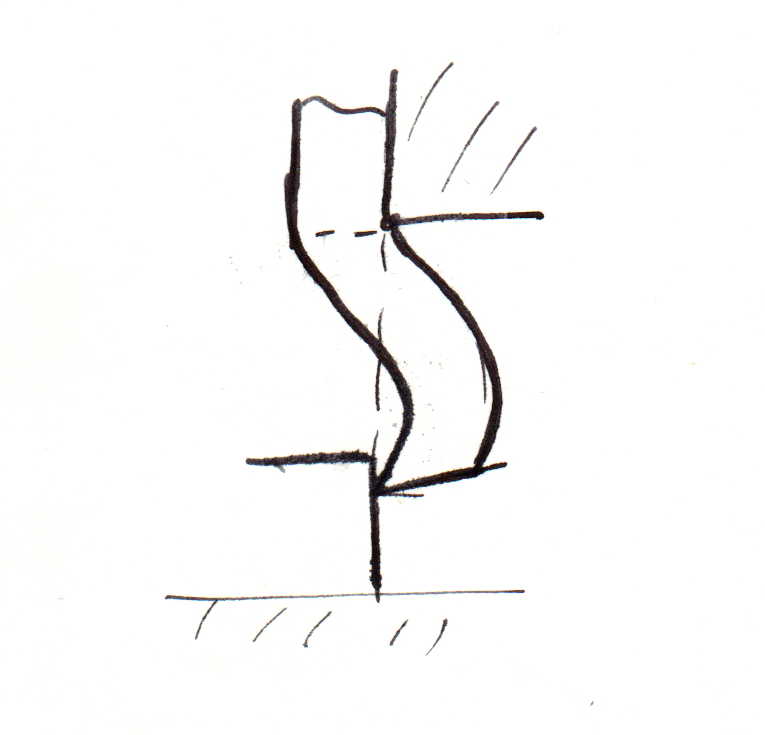
\includegraphics[scale=0.15]{image_16-3.png}
\end{figure}
\FloatBarrier
Za učvršćenje noževa postoje i posebne glave koje omogućavaju stezanje noževa i pod kutem.
\section{Tokarenje}
Tokarski strojevi su strojevi koji spadaju u najpotrebnije strojeve bilo kakove metaloprerađivačke industrije. Oni posjeduju veliku univerzalnost jer je na njima moguće obrađivati: ravne i zakrivljene površine, mogu se rezati narezi, bušiti i zakrivljene površine, mogu se rezati plohe, razvrtati, irzrađivati spiralne opruge, glodati horizontalne utore itd. Tokarski strojevi su veoma jednostavni a predmet koji obrađujemo dobro se vidi. Alati su jednostavni, jeftini i mogu se brzo i lako postavljati i skidati.\par
Kod tokarskih strojeva glavno kretanje vrši predmet i to rotira. Posmak vrši nož, a tokarski stroj obično ima samo jedan. Da bi se povečala produktivnost stroja, a posebno kod velikih tokarski strojeva obrada se može vršiti i s dva ili više noževa. No takove mogućnosti, strojevi imaju po dva suporta a katkada se na jednom suportu, ali s dvije strane postavljaju noževi.\par 
Mane tokarskih strojeva su:
\begin{itemize}
\item obrada se često vrši samo jednom oštricom i zato je potrebno često prebrušavanje.
\item ako je predmet nepravilnog oblika njegovo učvršćivanje na stroj je nezgodno.
\item otežano centriranje predmeta što traži više vremena pa je skupo
\item stroj zauzima relativno mnogo mjesta.
\end{itemize}
\par
Prednosti tokarskog stroja su:
\begin{itemize}
\item jednostavno rukavanje strojem.
\item jednostavni i jeftini alati
\item preglednost obrade
\item univerzalnost obrade koju smo već prije spomenuli.
\end{itemize}
\par
Opčenito gledajući, svi tokarski strojevi su jednaki. Jedan od drugoga se razlikuju po broju radnih brzina i posmaka, veličinom instalirane snage i masivnošću. To vrijedi za obične tokarske strojeve. Za specijalne svrhe razvijen je čitav niz tokarskih strojeva.Sve to nas upučuje na to da tokarske strojeve podijelimo na:
\begin{enumerate}
\item \textbf{Jednostavne tokarske strojeve}\\
Koji mogu biti:
\begin{itemize}
\item Tokarski strojevi s nareznim vretenom
\item Tokarski strojevi s poteznim vretenom
\item Tokarski strojevi s poteznim i nareznim vretenom.
\end{itemize}
\item \textbf{Specijalni tokarski strojevi}\\
S obzirom na specijalnost oni se dijele na:
\begin{itemize}
\item Obične specijalne tokarske strojeve
\begin{itemize}
\item za čeona tokarenja - čeoni tokarski stroj (301 str.)
\item Korusel tokarski stroj (302 str.)
\item tokarski stroj za profilno tokarenje (303 str.)
\item tokarski stroj za tokarenje željezničkih kotača (305 str.)
\item tokarski stroj za natražno tokarenje (307 str.)
\item tokarski stroj za obradu koljeničastih osovina (308 str.)
\item tokarski stroj za odrezivanje (309 str.)
\end{itemize}
\item Revolverski tokarski stroj - strojevi s više alata na tkz. revolverskoj glavi za mijenjanje alata
\item Poluautomatski tokarski stroj - tu spadaju agregatni strojevi
\item Automatski tokarski strojevi - sa jednim ili više vretena koji mogu biti upravljani numeričkim ili računalnim programom
\end{itemize}
\end{enumerate}
Tokarski stroj se sastoji od četiri glavna dijela:
\begin{enumerate}
\item Radno vreteno sa sistemom prijenosa od el. motora do radnog vretena, koje se naziva vretenište.
\item Postolje tokarskog stroja sa saonicama po kojima kliže suport i konjić
\item Suporti (obično poprečni ili uzdužni) s napravom za stezanje noža, koji preuzimaju pogon od vučnog ili navojnog vretena i ostvaruju posmak
\item Konjić sa šiljkom za učvršćivanje predmeta.
\end{enumerate}
Kod tokarskih strojeva je konjić uvijen s desne strane radnika, a vretenište sa steznom glavom lijevo od radnika, za vrijeme rada.\par
Numerički ili računalno upravljani strojevi uz te dijelove imaju i jedinice za upravljanje strojem. \par
Kada se govori o nekom tokarskom stroju onda se misli na njegove karakteristične podatke a to su:
\begin{enumerate}
\item visina radnog vretena iznad postolja, što definira maksimalni promjer tokarenja
\item razmak vrha glavnog vretena i vrha konjića, što definira maksimalna dužina uzdužnog tokarenja
\item snaga elektromotora s eventualnim stepenicama broja okretaja samog el. motora što je veoma rijetko. Obično je motor s jednim brojem okretaja.
\item broj radnih brzina koje je moguće ostvariti korz vretenište.
\end{enumerate}
\subsection{Uređaji za stezanje}
Da bi se predmet obradio na tokarskom stroju potrebno ga je učvrsiti u radno vreteno. Način učvršćivanja ovisi o obliku predmeta koji se obrađuje i o opremljenosti stroju na kojem ćemo predmet obrađivati. Tako raspoznajemo različite načine učvršćivanja stroja.
\clearpage
\subsubsection{Učvršćivanje predmeta između šiljaka radnog vretena i konjića}
\begin{figure}[!h]
\centering
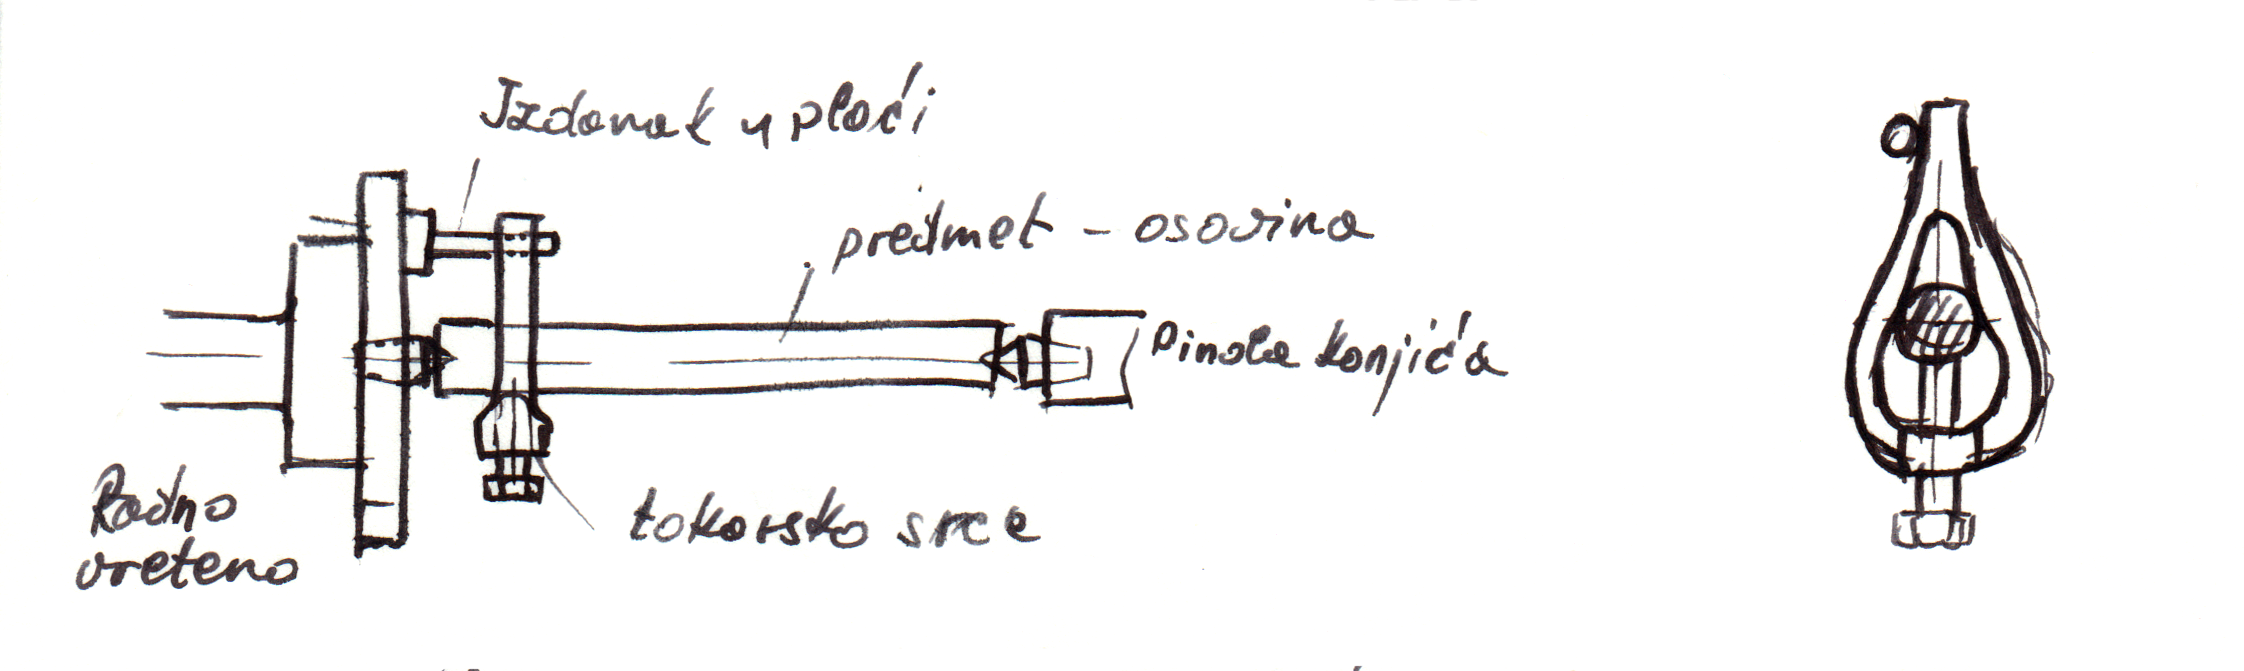
\includegraphics[width=0.8\textwidth]{image_18-1.png}
\end{figure}
\FloatBarrier
\par
Na kraju predmeta su zabušene posebne vrste rupa za centriranje i predmet je upet između šiljaka. Da bi se osiguralo njegovo zakretanje, na osovinu se montira uređaj koji se zove \textbf{tokarsko srce}. Svojim tlačnim vijkom tokarsko srce se učvrsi na predmet a svojim dužim krajem zapne za izdanak na ploči i na taj način vrti predmet.\par
Postoje dvije vrste šiljaka za takav način učvršćenja predmeta i to:
\begin{itemize}
\item čvrsi šiljci - za veoma fina tokarenja i lakše predmete
\item zakretni šiljci - koji se okreću zajedno s predmetom a pritisak se prenosi preko kugličnih ležajeva.
\end{itemize}
Ukoliko se bušenje predmeta, izrade središnjih provrta za šiljke, izvodi na tokarskom stroju, za pridržavanje predmeta koriste se linete. Postoje takozvane čvrste ili pomične linete sa valjcima.
\begin{figure}[!h]
\centering
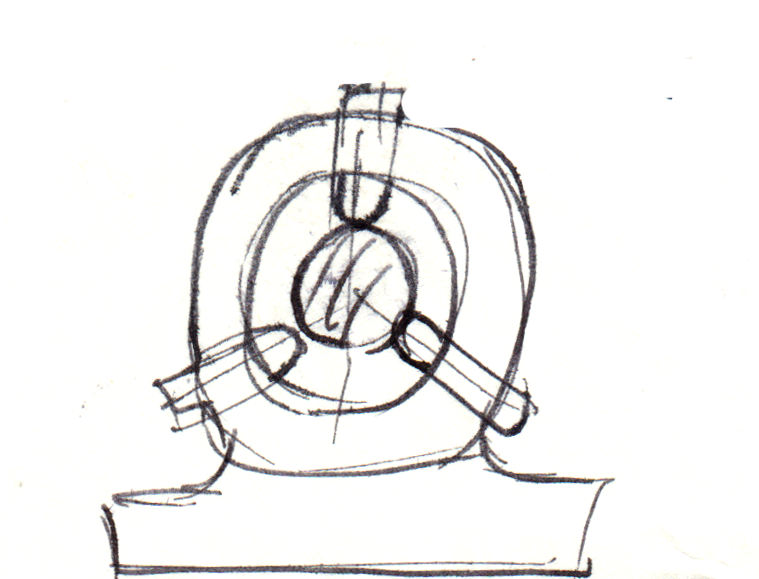
\includegraphics[scale=0.1]{image_18-2.png}
\end{figure}
\clearpage
\subsubsection{Učvršćenje predmeta pomoču čeljusne ploče}
\begin{figure}[!h]
\centering
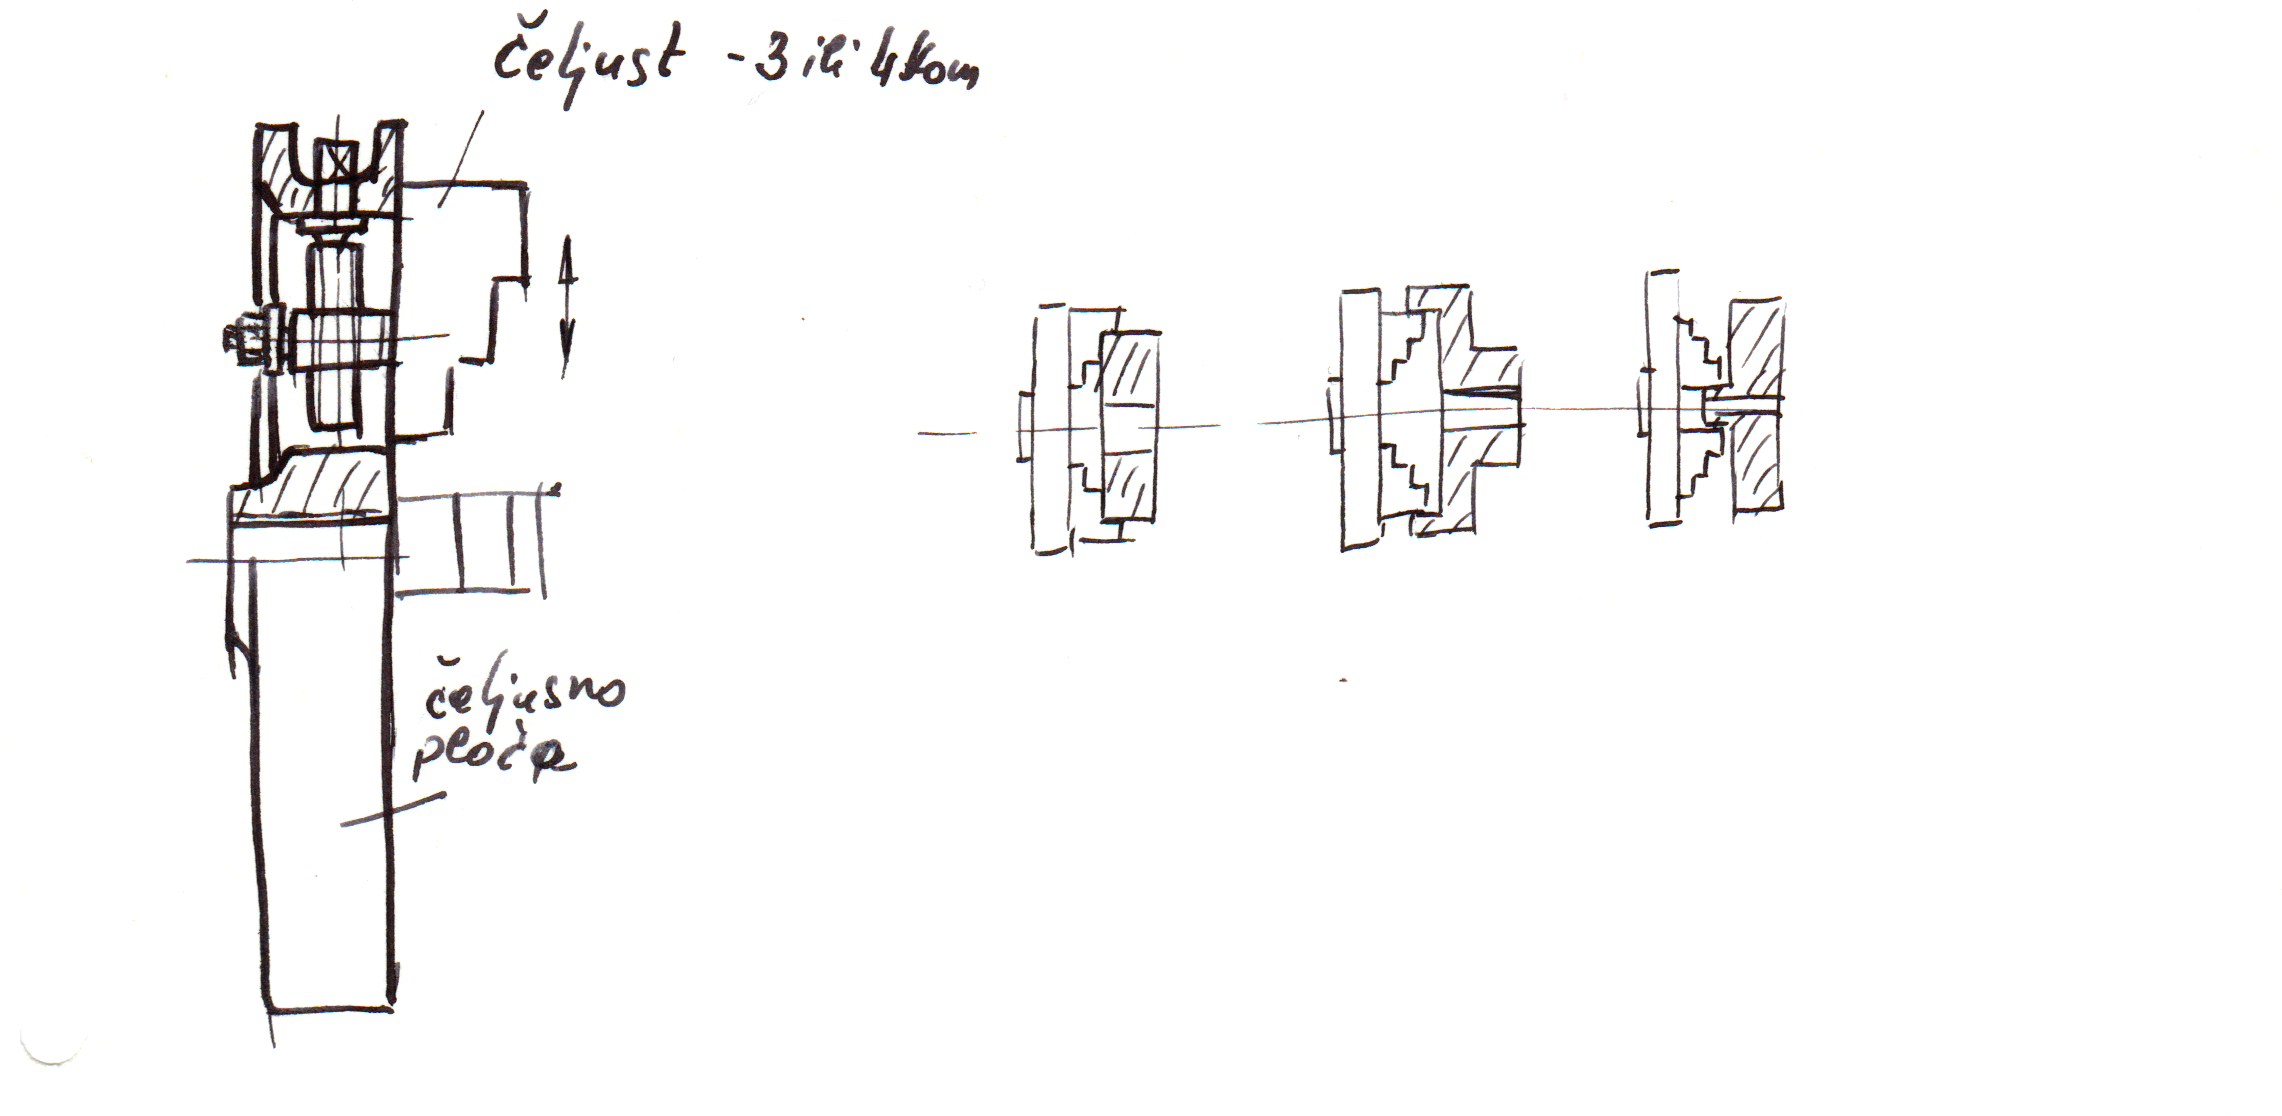
\includegraphics[width=0.8\textwidth]{image_19-1.png}
\end{figure}
\FloatBarrier
Na čeljusnoj ploči postoje obično 3 ili 4 čeljusti koje se mogu neovisno jedno od druge, sa svojim vijkom za podešavanje, pomicati duž posebnog kanala u ploči. Ovaj način se koristi kod nesimetričnih oblika koji se moraju tokariti. Postoje uređaji na steznim pločama koji su ugrađeni u stezne ploče, da se prilikom otezanja  jedne čeljusti stežu jednoliko sve tri čeljusti. Takove stezne ploče nazivamo \textbf{amerikanerima}. Danas već postoji čitav niz riješenja amerikanerima. (Horvat 294. - 295. str.)\par
Osim ova dva načina pritezanja, danas postoje i pričvršćenje elektromagnetima i pneumatski ili ihraulično pritezanje.
\subsection{Pričvršćenje noževa}
Danas se učvršćenje noževa izvodi u malim napravicama koje mogu primiti i 4 noža a mogu se zakretati oko svog središta. Te napravice su učvršćene nas suportu stroja.
\begin{figure}[!h]
\centering
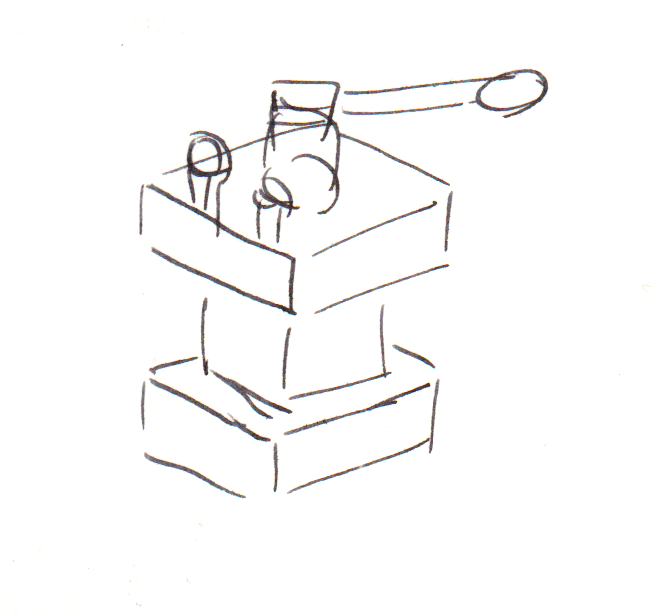
\includegraphics[scale=0.1]{image_19-2.png}
\end{figure}
\FloatBarrier
\subsection{Tokarski noževi} 
\begin{enumerate}
\item Ručni tokarski noževi (Horvat 234.):
\begin{itemize}
\item za glađenje
\item za odrezivanje
\item za urezivanje
\item za unutarnji narez
\item za vanjski narez.
\end{itemize}
\item Strojni tokarski noževi - upeti u suportu:
\begin{itemize}
\item tokarski noževi od jednog komada
\item tokarski noževi s navarenom oštricom (244. str.)
\item tokarski noževi s držačima oštrice (245. - 248. str.).
\end{itemize}
Tokarske noževe dijelimo na :
\begin{itemize}
\item noževi za vanjsko tokarenje
\item noževi za unutarnje tokarenje.
\end{itemize}
Sljedeća podjela noževa je:
\begin{itemize}
\item noževi za grubo obrađivanje - Klapstokor nož (52 sl. 70 str.)
\item noževi za fino obrađivanje
\item noževi za postrana obrađivanja (grubo ili fina)
\item noževi za utore i odrezivanja
\item profilni noževi (okrugli fazonski nož sl. 250. str. 240.)
\item noževi za izrađivanje nareza
\item uz odgovarajuće noževe vanjsko tokarenje imamo tako i noževe za unutarnja tokarenja.
\end{itemize}
\end{enumerate}
\subsubsection{Režimi i njihovo određivanje}
Režimi ovise o nizu faktora:
\begin{itemize}
\item materijalu kakav obrađujemo
\item da li obrađujemo grubo ili fino
\item s kakvim nožem vršimo obradu.
\end{itemize}
Iz brzine rezanja i promjera obrađivanog predmeta odabiremo broj okretaja tokarskog stroja. Preko mjenjačke kutije, nekada poznati Norton odredimo broj okretaja stroja i veličinu poznatu uz odabranu dubinu rezanja.
\subsubsection{Sile rezanja na tokarskom nožu}
O sili rezanja već smo prije opširno govorili.
\subsubsection{Tokarenje konusa na tokarskom stroju}
Možemo ga izvesti:
\begin{enumerate}
\item Zakretanjem pomoćnog uzdužnog suporta za kut nagiba konusa (Horvat 259. str.)
\item Izbacivanje središnjeg šiljka na konjića iz simetrale stroja
\begin{figure}[!h]
\centering
\includegraphics[width=0.8\textwidth]{image_20.png}
\end{figure}
\FloatBarrier
\item Pomoću Kapirne letve (Horvat 283. sl. - 261. str.).
\end{enumerate}
Tokarenje navoja, bilo vanjski ili unutarnji moguće je izvesti za pale proreze pomoću konjića kojim pritiskujemo navojno svrdlo ili utezima (Horvat 263. str. 286 slika), a kod tokarenja velikih nareza svih oblika koristimo kalibrirane noževe. Brušenje centralnih provrta vrši se pomoću konjića u koji se umetne svrdlo.\par
Brušenje vanjsko ili unutarnje vrši se tako da se nasuprot učvrsti odgovarajući nosač brusne ploće i vršsi brušenje. Kod velikih strojeva postoji čitav niz alata i naprava za najrazličitije svrhe:
\begin{itemize}
\item glodanje uzdužnih utora
\item brušenje provrta na prirubnicama
\item brušenje svih vrsta
\item razvrtavanje itd.
\end{itemize}
\subsubsection{Vrijeme obrade na tokarskom stroju}
Kao i svaka norma i ova se sastoji od niza međusobno manje ili više vezanih detalja.
\begin{enumerate}
\item Pripremno vrijeme
\item Čisto strojno vrijeme koje se može odrediti iz odabranih režima rada (brzine rezanja, posmaka i dubine rezanja). A dijeli se na strojno vrijeme, strojno ručno vrijeme i radno vrijeme.
\item Završno vrijeme
\item Dodatno vrijeme
\begin{itemize}
\item Ku - faktor zamora
\item Ka - faktor koji na čovijeka registrira utjecaj okoline
\item Kd - dopunsko vrijeme (propisani odmor, osobne potrebe, organizirani gubitci).
\end{itemize}
Sve to vrijedi za prosječno uvježbanog čovjeka.
\end{enumerate}
\begin{table}[!h]
\centering
\caption{Alati od tvrdih metala}
\label{my-label}
\begin{tabular}{cc|c|c|}
\cline{3-4}
\multicolumn{1}{l}{}                   & \multicolumn{1}{l|}{}                    & \multicolumn{2}{c|}{Brzina rezanja}                                  \\ \hline
\multicolumn{1}{|l|}{Materijal obrade} & \multicolumn{1}{l|}{Čvrstoća materijala} & \multicolumn{1}{l|}{Gruba obrada} & \multicolumn{1}{l|}{Fina obrada} \\ \hline
\multicolumn{1}{|c|}{Če 37}            & 37-42                                    & 180-250                           & 250-350                          \\ \hline
\multicolumn{1}{|c|}{Če 60}            & 60 - 70                                  & 100 - 130                         & 130 - 170                        \\ \hline
\multicolumn{1}{|c|}{Cr-Ni}            & 70 - 85                                  & 80 - 100                          & 100 - 120                        \\ \hline
\multicolumn{1}{|c|}{Nehrđajuči}       & 60 - 70                                  & 40 - 60                           & 60 -90                           \\ \hline
\multicolumn{1}{|c|}{Cr - V -čelici}   & 100                                      & 25 - 45                           & 45 - 80                          \\ \hline
\multicolumn{1}{|c|}{12\% Mn}            &                                          & 10 -25                            & 25 - 40                          \\ \hline
\multicolumn{1}{|c|}{Če - lijev}       & 40 - 50                                  & 90 - 120                          & 120 - 160                        \\ \hline
\end{tabular}
\end{table}
\FloatBarrier
\section{Bušilice}
Bušilice su strojevi, čiji naziv govori o samoj namjeri. One buše provrte u predmetu. Modernije izvedbe bušilica imaju mogučnost narezivanja, razvrtavanja i glodanja. \par
Predmet je redovito čvrsto upet na radnom mjestu, a svrdlo vrši sva druga gibanja, glavno rotiranje oko svoje osi i pomično - aksijalno savladavanje otpora aksijanlnog prodiranja u materijal. 
Prva podjela bušilica je:
\begin{itemize}
\item ručne koje unutar sebe možemo podijeliti na:
\begin{itemize}
\item ručni uređaji za bušenje
\item ručni uređaji s pogonom na elek. struju ili komprimirani zrak
\item uređaji za bušenje sa zmijastom osovinom (danas se to koristi za izvijaće).
\end{itemize}
\item strojne koje dalje dijelimo na:
\begin{itemize}
\item obične bušilice - za rad sa spiralnim svrdlom koje je učvršćeno u vreteno bušilice
\item bušilice za povečanje postojećeg provrta - koje rade motkama za brušenje s učvršćenim nožom.
\end{itemize}
\end{itemize} 
Prema načinu rada bušilice dijelimo na
\begin{itemize}
\item bušilice s okomitim vretenom koje se dijele na stolne bušilice, konzolne ili radijalne bušilice raznih veličina i viševretene bušilice.
\end{itemize}
Kod bušilica razlikujemo dva osnovna tipa.
\begin{figure}[!h]
\centering
\includegraphics[width=0.9\textwidth]{image_21.png}
\end{figure}
\FloatBarrier
Razlika između ova dva tipa  bušilica je u tome što je stup prve bušilice okrugli a sradni stol se uz vertikalno pomicanje gore dolje može zakretati oko stupa. Te bušilice se nazivaju još i stolnim bušilicama. \par
Druga izvedba bušilica je takova što na stupu ima vodilice za vertikalno pomicanje glave gore dolje, dok je stol stabilani čvrst. \par
Na trećoj skici slaba nam je specijalna izvedba bušilice tkz. \textbf{radijalna bušilica}. Ovaj tip bušilica obično su one večih dimenzija, obično se koriste kod bušenja provrta na velikim predmetima koje je nemoguće premještati pod pinolu svrdla. Ta bušilica sastoji se od postolja, okruglog stupa, u kojem se giba konzola gore-dolje i zakreće oko okruglog stupa, konzole po kojoj se ljevo desno giba nosač alata koji u sebi ima pogonska vretena koje se opet giba gore dolje i vrši glavno gibanje kretanja alata - rotaciju. Uz ovakvu bušilicu ide i postolje koje se može odkloniti. Veličina bušilice definirana je prema največev mogučem svrdlu odnosno prema največoj mogučoj izbušenoj rupi. Stepenovanje bušilica izgleda odprilike ovako:
\begin{center}
6, 10, 16, 25, 32, 40, 50, 63, 80 mm
\end{center}
Posoje DIN standardi kod kojih su definirane neke mjere pa je tako u ovisnosti o maksimalnom promjeru svrdla definirani i drugi podatci a to su:
\begin{itemize}
\item vertikalni hod vretena 80 - 400 mm
\item razmaka od temeljne ploće do vretena do 1320 mm
\item minimalna brzina rezanja kod nazivnoh promjera  35 - 10 m/min
\item minimalan automatski posmak 0,1 - 0,4 mm/okr
\item trajna snaga 0,2 - 12 kW
\end{itemize}
\subsection{Viševretene bušilice}
Koriste se kod serijske proizvodnje proizvoda sa više provrta (prirubnice, blokovi motora itd.) Specifičnost prigona je u tome što svako vreteno ima zglobnu vezu s glavnom pogonskom osovinom, ali sama svrdla se mogu postaviti u razne međusobne položaje.
\subsection{Koordinatna bušilica}
Za najtočnija obrađivanja. Ovdje se pomiče i stol na kojem je učvršćen predmet. Uz translatorna gibanja može se i zakretati. Nosač alata se također pomiče pa možemo dobiti točne kordinate položaja. Mogučnost optičkog postavljanja je i do 0,001 mm. Koriste se za izradu alata i naprava, a mora biti u klimatiziranoj prostoriji. Građena je veoma robusno, da se izbjegnu bilo kakve deformacije usljed sila rezanja koje se moraju kretati u donjim graničnim veličinama.
\subsection{Alati za bušenje i razvrtanje}
Princip rada alata je u tome da on vrši glavno kretanje i posmak - pomicanje u smjeru alata.
\begin{enumerate}
\item \textbf{Obično svrdlo} - jednostavno i jeftino. Teško odvođenje strugoine, svrdlo pobjegne u stranu.
\begin{figure}[!h]
\centering
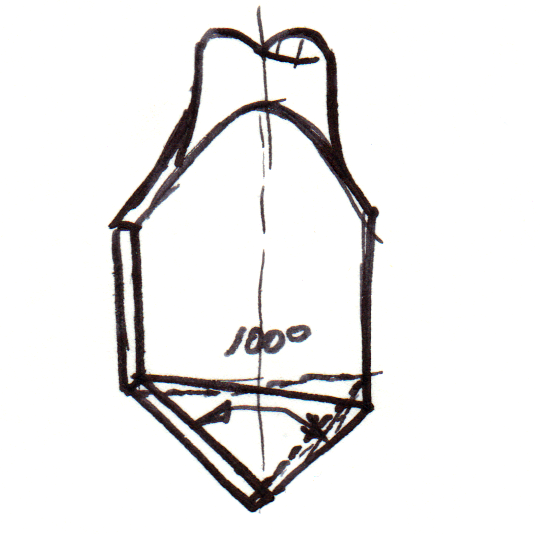
\includegraphics[scale=0.12]{image_22-1.png}
\end{figure}
\FloatBarrier
\item \textbf{Spiralno svrdlo} - uveo Modse - Sad. Veči učinak svrdla i dobro pobjegne u stranu.
\begin{figure}[!h]
\centering
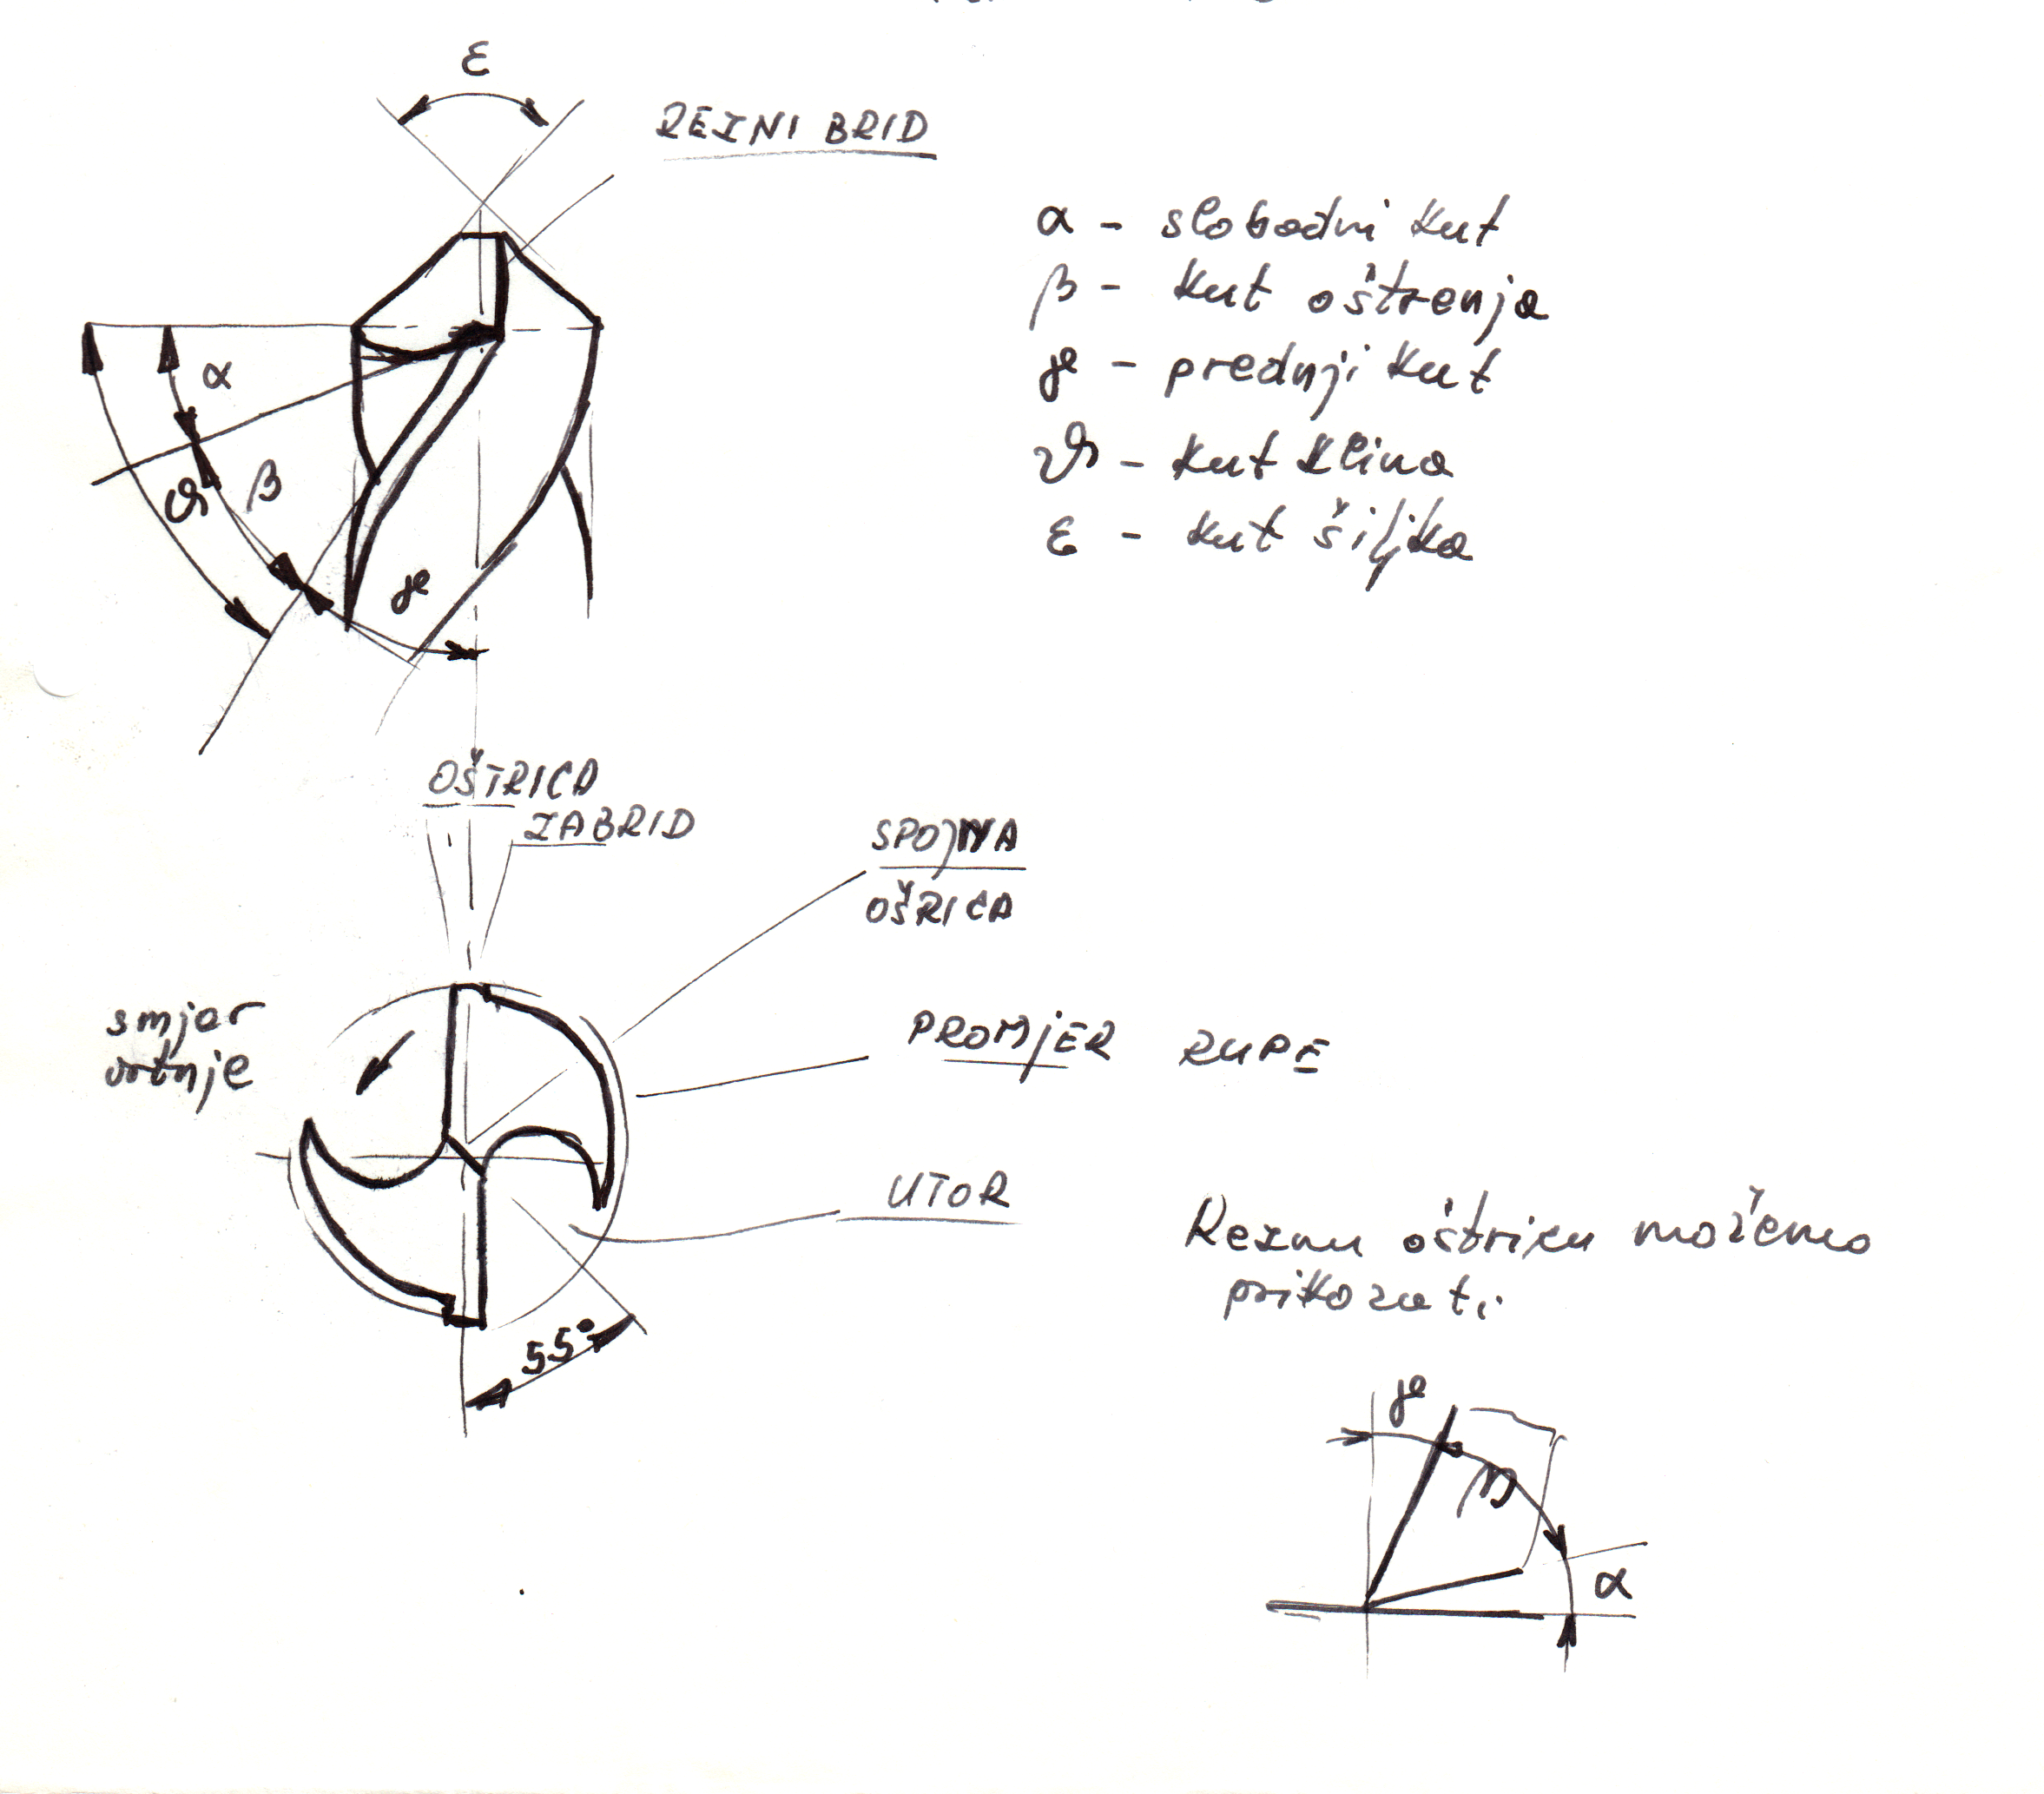
\includegraphics[scale=0.13]{image_22-2.png}
\end{figure}
\FloatBarrier
\end{enumerate}
Spojna oštrica, zbog svog oblika i veličine preuzima oko 40\% ukupne vertikalne sile koja se javlja pri bušenju. Ta bi se ta sila smanjila prelazima prebrušavanja i smanjenju te oštrice. Poznato je više načina, a jedan sljedići je prikazan skicom.
Kod brušenja velikih provrta utijecaj spojne oštrice se izbjegava na taj način da se prvo izbuši provrt sa malim svrdlom a onda sa velikim.
\begin{figure}[!h]
\centering
\includegraphics[scale=0.15]{image_23.png}
\end{figure}
\FloatBarrier
Kod bušenja - provrt nema u principu izlaz veći od promjera svrdla. Kod mekanih materijala je to nadmjera veća nego kod krtih. Nadmjera je veća kod većih promjera.
\subsection{Brzina rezanja}
Zbog oblika i načina rada svrdlo duž oštrine se režim rada mijenja, to prvo dolazi do zatupljenja perifrenih rubova svrdla. Veličina aksijalnih sila i brzine rezanja ovise o 
\begin{itemize}
\item materijal koji bušimo
\item materijal svrdla
\item promjer svrdla
\item posmak svrdla koji djelimo na dvije oštrice
\item širi spojne oštrice 
\item hlađenju - mazanju
\item veličini vršnog kuta i nagibu zavojnice.
\end{itemize}
Trajanje oštrice svrdla naglo pada s povećanjem brzine rezanja.\par
Za bušenje tvrdog lijeva, kaljenog čelika, manganovog čelika, stakla, porculana, plastičnih masa i mramora koriste se svrdla s umetnutim pločicama (widia). Kod tih svrdala, koriste se velike brzine rezanja ali minimalni posmaci.\par
Produktivnost bušilice mjeri se u količini izbušenog materijala u jedninici vremena. Ovdje moramo voditi računa o ekonomičnosti, pa postoji gornja granica veličine posmaka. Preveliki posmak izaziva
\begin{itemize}
\item previsoku aksijanu silu
\item prebrzo istrošenje oštrice
\item preveliko opterećenje stroja, deformacije predmeta, dobivamo lošu izrađevinu.
\end{itemize}
Ovisnost posmaka i promjera svrdala vezanih u vrste materijala.
\begin{figure}[!h]
\centering
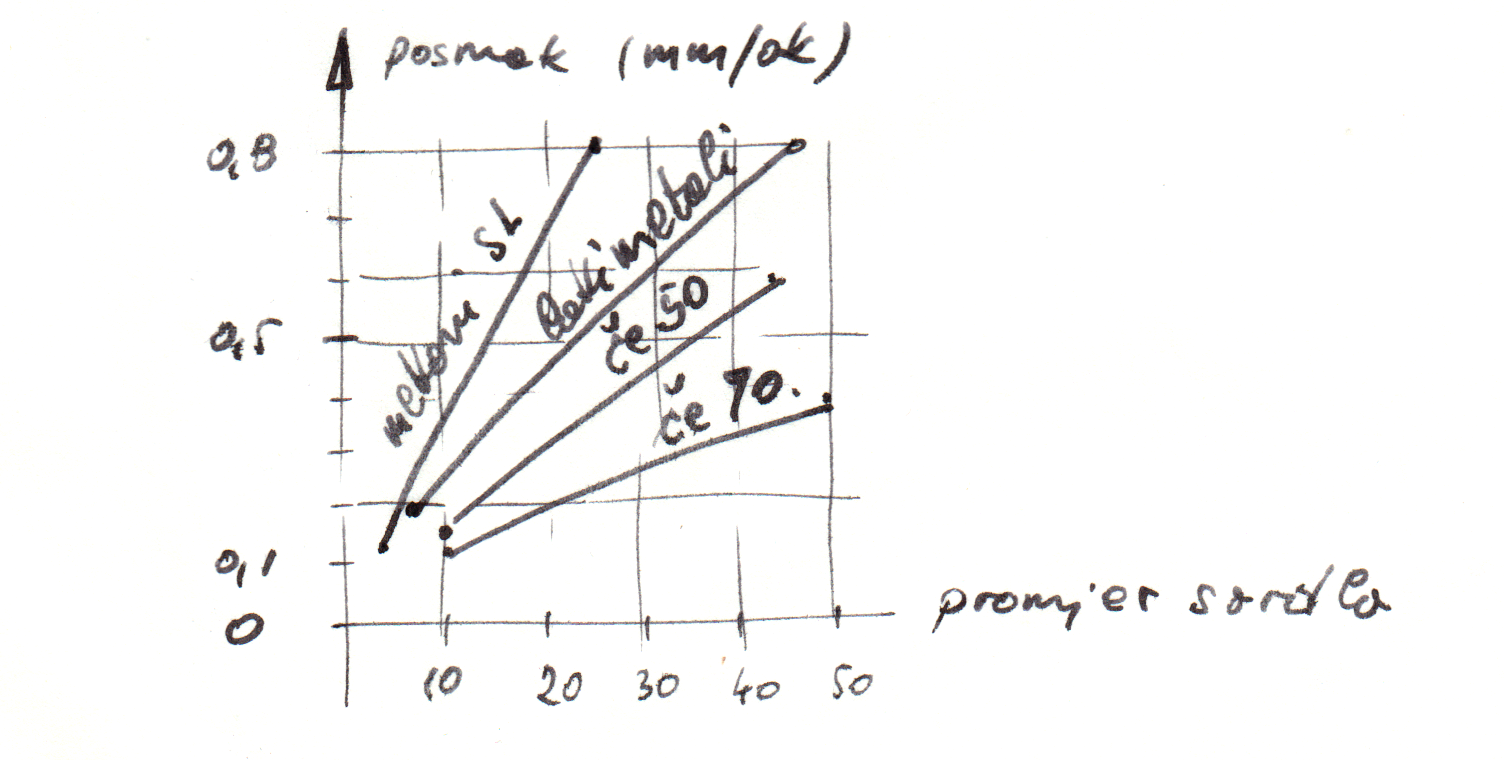
\includegraphics[scale=0.13]{image_24-1.png}
\end{figure}
\FloatBarrier
Uz plosnato i spiralno glodalo od najpoznatijih su još
\begin{figure}[!h]
\centering
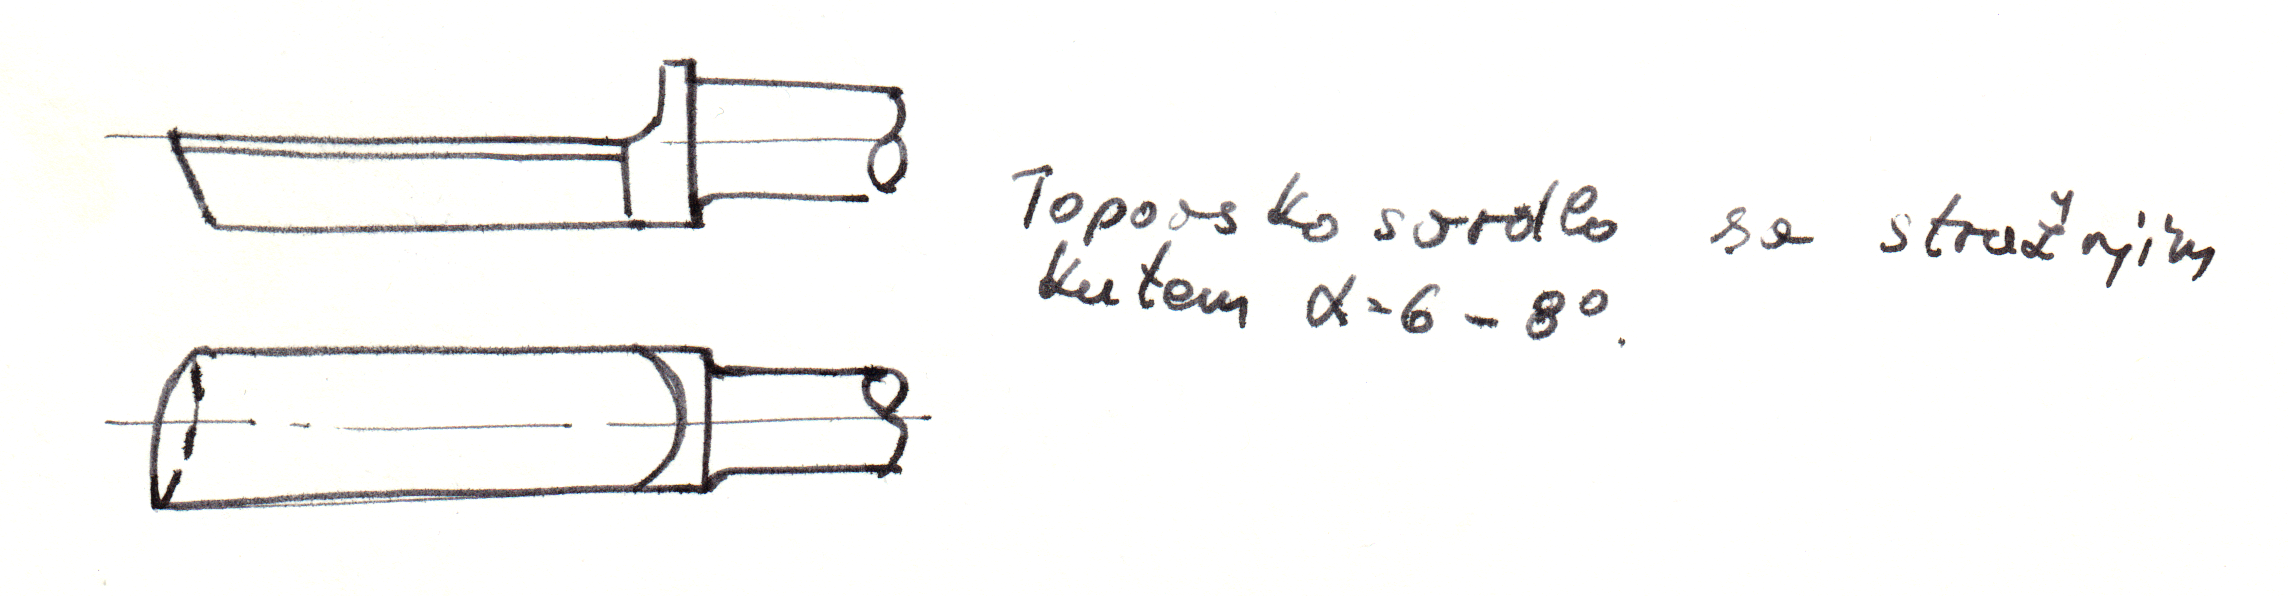
\includegraphics[scale=0.13]{image_24-2.png}
\end{figure}
\FloatBarrier

Upuštala za izradu cetričnih ili središnjih provrta. Kao tokarenja na šiljcima ili za učvršćenje u konjić.
\begin{figure}[!h]
\centering
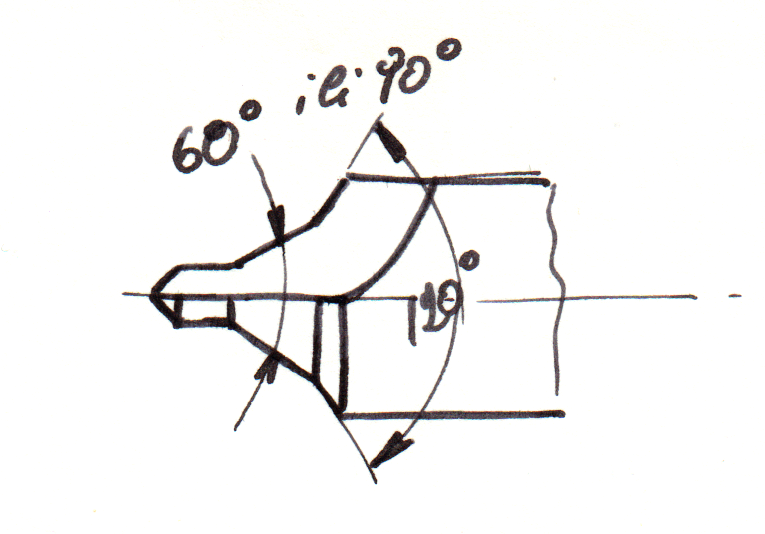
\includegraphics[scale=0.13]{image_25-1.png}
\end{figure}
\FloatBarrier
Postoje spiralana svrdla čije su oštrice napravljene od widia pločica. Postoji također i trobridno widi svrdla.
\begin{figure}[!h]
\centering
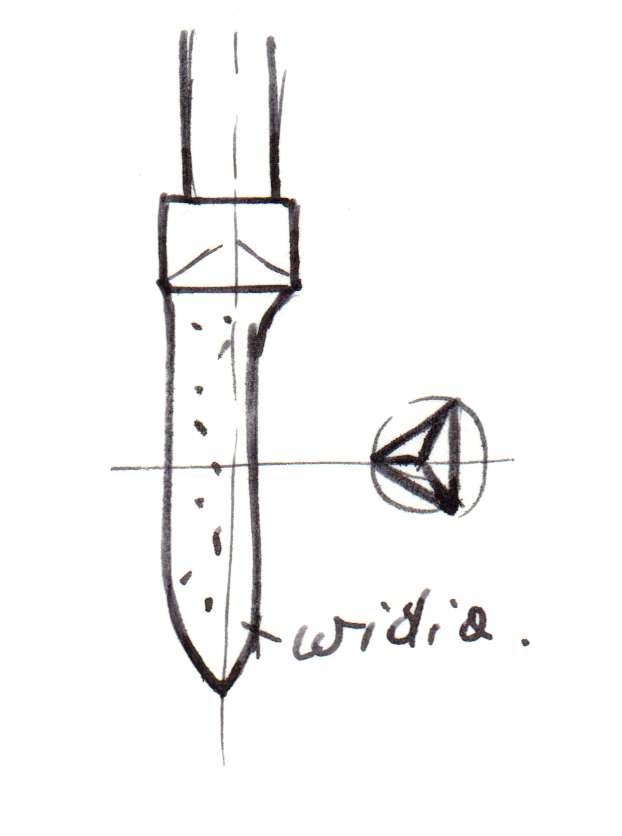
\includegraphics[scale=0.1]{image_25-2.png}
\end{figure}
\FloatBarrier
\subsection{Upuštala}
Jedan od čestih alata s kojima se susrečemo na bušilicama su upuštivači za upuštanje rubova, skidanje srha, proširenje rupa itd.
\begin{figure}[!h]
\centering
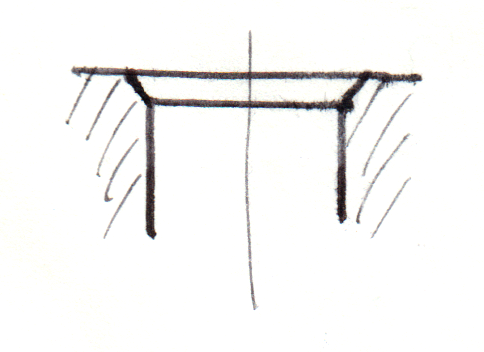
\includegraphics[scale=0.13]{image_25-3.png}
\end{figure}
\FloatBarrier
Jedan od čestih upuštala
\begin{figure}[!h]
\centering
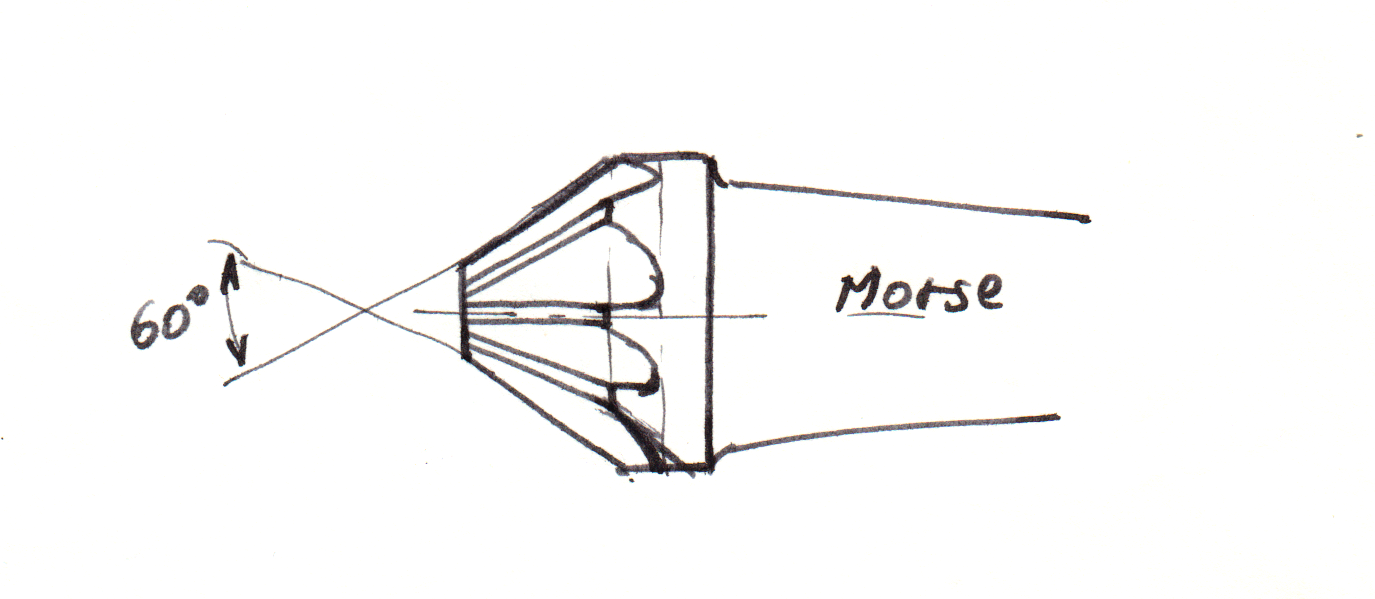
\includegraphics[scale=0.13]{image_25-4.png}
\end{figure}
\FloatBarrier
Ostali oblici u Hribar 58.
\subsection{Razvrtavači}
Za dotjerivanje provrta, postizanje većih točnosti, za stvaranje malih koničnosti koriste se razvrtači. Razlikujemo razvrtala za ručni i strojni rad. Druga razdioba razvrtača može se  uzeti kao:
\begin{itemize}
\item razvrtala s krutim zupcima
\item razvrtala s udesivim zupcima
\end{itemize}
Razvrtala u pravilu imaju paran broj zubaca zbog fizikalnih potreba jednolikog opterečenja svih zubaca. U principu razvrtala se gledaju kao jedna oštrica s konturom.
\begin{figure}[!h]
\centering
\includegraphics[scale=0.13]{image_26.png}
\end{figure}
\FloatBarrier
\noindent Na strojevima se koriste trostepeni konični razvrtači (početni srednji i završni) Hribor 62 str.
\clearpage
\subsection{Učvršćenje svrdla u radna vretena}
Način učvršćenja svrdala vezan je uz veličinu provrta koju svrdlo buši. Kod manjih provrta manje su sile rezanja, manji zakretni momenti a to veličine rastu s porastom promjera svrdla. Zbog toga je dio svrdla koji se učvrščuje različito izveden.
\begin{figure}[!h]
\centering
\includegraphics[scale=0.13]{image_27.png}
\end{figure}
\FloatBarrier
Ovisno o veličine bušilice, radno vreteno ima u sebi pripremljeni odgovorajući Morse Konus. Da bi se u takvo radno vreteno umetnulo i manje svrdlo, koriste se redukcione čahure Mores Konus. Morse Konus drži svrdlo sa principu trenja. Drugi način učvršćenja svrdla sa cilindričnim završetkom je pomoću posebno konstruiranih glava za zatezanje. Postoji čitav niz takvih glava, a sada se koriste i glave koje rotiraju, i u rotaciji je moguće izvesti zamjenom svrdala.
\subsection{Režimi obrade kod brušenja}
Ekonomska brzina rezanja - brušenja je ona brzina kad svrdlo može izbušiti ukupno 2000 mm dubine. Ta brzina onačava se kao $\nu_{r}=2000$.\par
Ovisno o vrsti materijala koju bušimo razlikujemo način brušenja oštrica svrdala. Osim toga za različite materijale nagib odvodne spirale je za svaki materijal drugačiji jer on bolje odvodi strugotinu. To je veoma važno kod brušenja dubokih provrta jer je onda izbjegnuto višekratno vađenje svrdala i češćenje koje smanjuje produktivnost. Stoga je taj detalj treba uvesti kod određivanja norme za bušenje dubokih provrta.
\begin{table}[!h]
\centering
\resizebox{\textwidth}{!}{%
\begin{tabular}{cccc|c|c|c|c|c|c|}
\cline{5-10}
\multicolumn{1}{l}{}                                                                             & \multicolumn{1}{l}{}                    & \multicolumn{1}{l}{}                & \multicolumn{1}{l|}{}                                                     & \multicolumn{6}{c|}{Posmak mm/ok}       \\ \cline{5-10} 
                                                                                                 &                                         &                                     &                                                                           & \multicolumn{6}{c|}{Promjer svrdla}     \\ \hline
\multicolumn{1}{|c|}{Materijal svrdla}                                                           & \multicolumn{1}{c|}{Rashladno sredstvo} & \multicolumn{1}{c|}{Brzina rezanja} & Brušenji materijal                                                        & 5    & 8    & 12   & 16   & 25   & 40   \\ \hline
\multicolumn{1}{|c|}{\multirow{3}{*}{\begin{tabular}[c]{@{}c@{}}Alatni\\ čelik\end{tabular}}}    & \multicolumn{1}{c|}{Sapunica}           & \multicolumn{1}{c|}{10-18}          & \begin{tabular}[c]{@{}c@{}}čelik do \\ 50 kp/mm$^{2}$\end{tabular}             & 0,09 & 0,12 & 0,16 & 0,18 & 0,2  & 0,22 \\ \cline{2-10} 
\multicolumn{1}{|c|}{}                                                                           & \multicolumn{1}{c|}{Rashladno sredstvo} & \multicolumn{1}{c|}{9-12}           & \begin{tabular}[c]{@{}c@{}}čelik iznad\\ 50 kp/mm$^{2}$\end{tabular}           & 0,08 & 0,11 & 0,14 & 0,16 & 0,18 & 0,2  \\ \cline{2-10} 
\multicolumn{1}{|c|}{}                                                                           & \multicolumn{1}{c|}{Suho}               & \multicolumn{1}{c|}{8-14}           & \begin{tabular}[c]{@{}c@{}}lijevano\\ željezo\\ do 18 kp/mm$^{2}$\end{tabular} & 0,12 & 0,18 & 0,22 & 0,25 & 0,3  & 0,35 \\ \hline
\multicolumn{1}{|c|}{\multirow{3}{*}{\begin{tabular}[c]{@{}c@{}}Brzorezni\\ čelik\end{tabular}}} & \multicolumn{1}{c|}{Sapunica}           & \multicolumn{1}{c|}{25-40}          &                                                                           & 0,11 & 0,16 & 0,22 & 0,25 & 0,3  & 0,4  \\ \cline{2-10} 
\multicolumn{1}{|c|}{}                                                                           & \multicolumn{1}{c|}{Rashladno sredstvo} & \multicolumn{1}{c|}{25-32}          &                                                                           & 0,1  & 0,14 & 0,18 & 0,2  & 0,3  & 0,4  \\ \cline{2-10} 
\multicolumn{1}{|c|}{}                                                                           & \multicolumn{1}{c|}{Suho}               & \multicolumn{1}{c|}{20-35}          &                                                                           & 0,16 & 0,25 & 0,3  & 0,35 & 0,45 & 0,5  \\ \hline
\end{tabular}%
}
\end{table}
\FloatBarrier
Brzina rezanja svrdla računa se na brzinu rezanja periferne oštrice svrdla i to 
\begin{equation}
v = \frac{D \cdot \pi}{4} \cdot \frac{n}{1000}\:,
\end{equation}
gdje je $D$ promjer svrdla u milimetrima, a $n$ je broj okretaja u min. Posmak se računa u mm/okretaj. U stvarnosti na svaku od oštrica odpada 1/2 posmaka za svrdlo s dvije oštrice dok je to 1/3 kod svrdala s tri oštrice.
\section{Brušenje}
Brušenje je vrsta obrade sa skidanjem strugotina. Strugotinu ne skidamo jednom oštricom, nego nizom nepravilno složenih i međusobno povezanih mineralnim zrncima, gdje svako zrnce predstavlja oštricu za sebe. Iako se radi o velikoj količini "oštrica", presjek strugotima mora biti minimalan jer su malene oštrice. Kada se takova oštrica, oštri rub mineralnog zrna zatupi, ona ispada iz cjeline, a pojavljuje se nova oštrica, novo mineralno zrno. Odpadanje mineralnih zrna, dovodi do promjena oblika brusnog alata kojeg je od vremena do vremena potrebno "prebrušavati", dotjerivati kvaliteti površinu.\par 
Brušenjem, zbog vemoa malog presjeka skidane površine, daje nam veoma glatke površine, a na taj način možemo dovesti obrađivane predmete u veoma uske granice tolerancije. \par
Tanke brusne ploće mogu veoma efikasno zamjeniti razne vrste pila za rezanje jer svojim velikim brzinama i produktivnošću to opravdavaju. \par
Uređaji na koje se učvršćuju brusevi alata nazivaju se brusilice.
\subsection{Brusilice}
Obzirom na oblik sredstva s kojim vršimo operaciju skidanja strugotina brusevima, razlikujemo dvije osnovne skupine brusilica:
\begin{enumerate}
\item Strojevi za brušenje brusnim pločama u koje spadaju
\begin{itemize}
\item strojevi za brušenje raznih površina
\item strojevi za okrugla brušenja koji se dijele na:
\begin{itemize}
\item strojevi za brušenje jednostavnih valjkastih predmeta
\item strojevi za brušenje složenih valjkastih predmeta
\item strojevi za unutarnje okruglo brušenje
\end{itemize}
\item strojevi za brušenje zupčanika
\item strojevi za brušenje alata
\item ostali specijalni strojevi za brušenje.
\end{itemize}
\end{enumerate}
\subsection{Brusilice za ravno brušenje}
Da bi obradili neku ravnu plohu brušenjem, koristimo brusnu ploču koja rotira oko svoje osi. Ako je os, oko koje se kreće brusna ploča horizontalna u tom slučaju površinu obrađujemo sa vanjskim rubom brusne ploče. Ako je os brusne ploče vertikalna u tom slučaju površinu obrađujemo čeonom površinom brusa. Tako razlikujemo
\begin{figure}[!h]
\centering
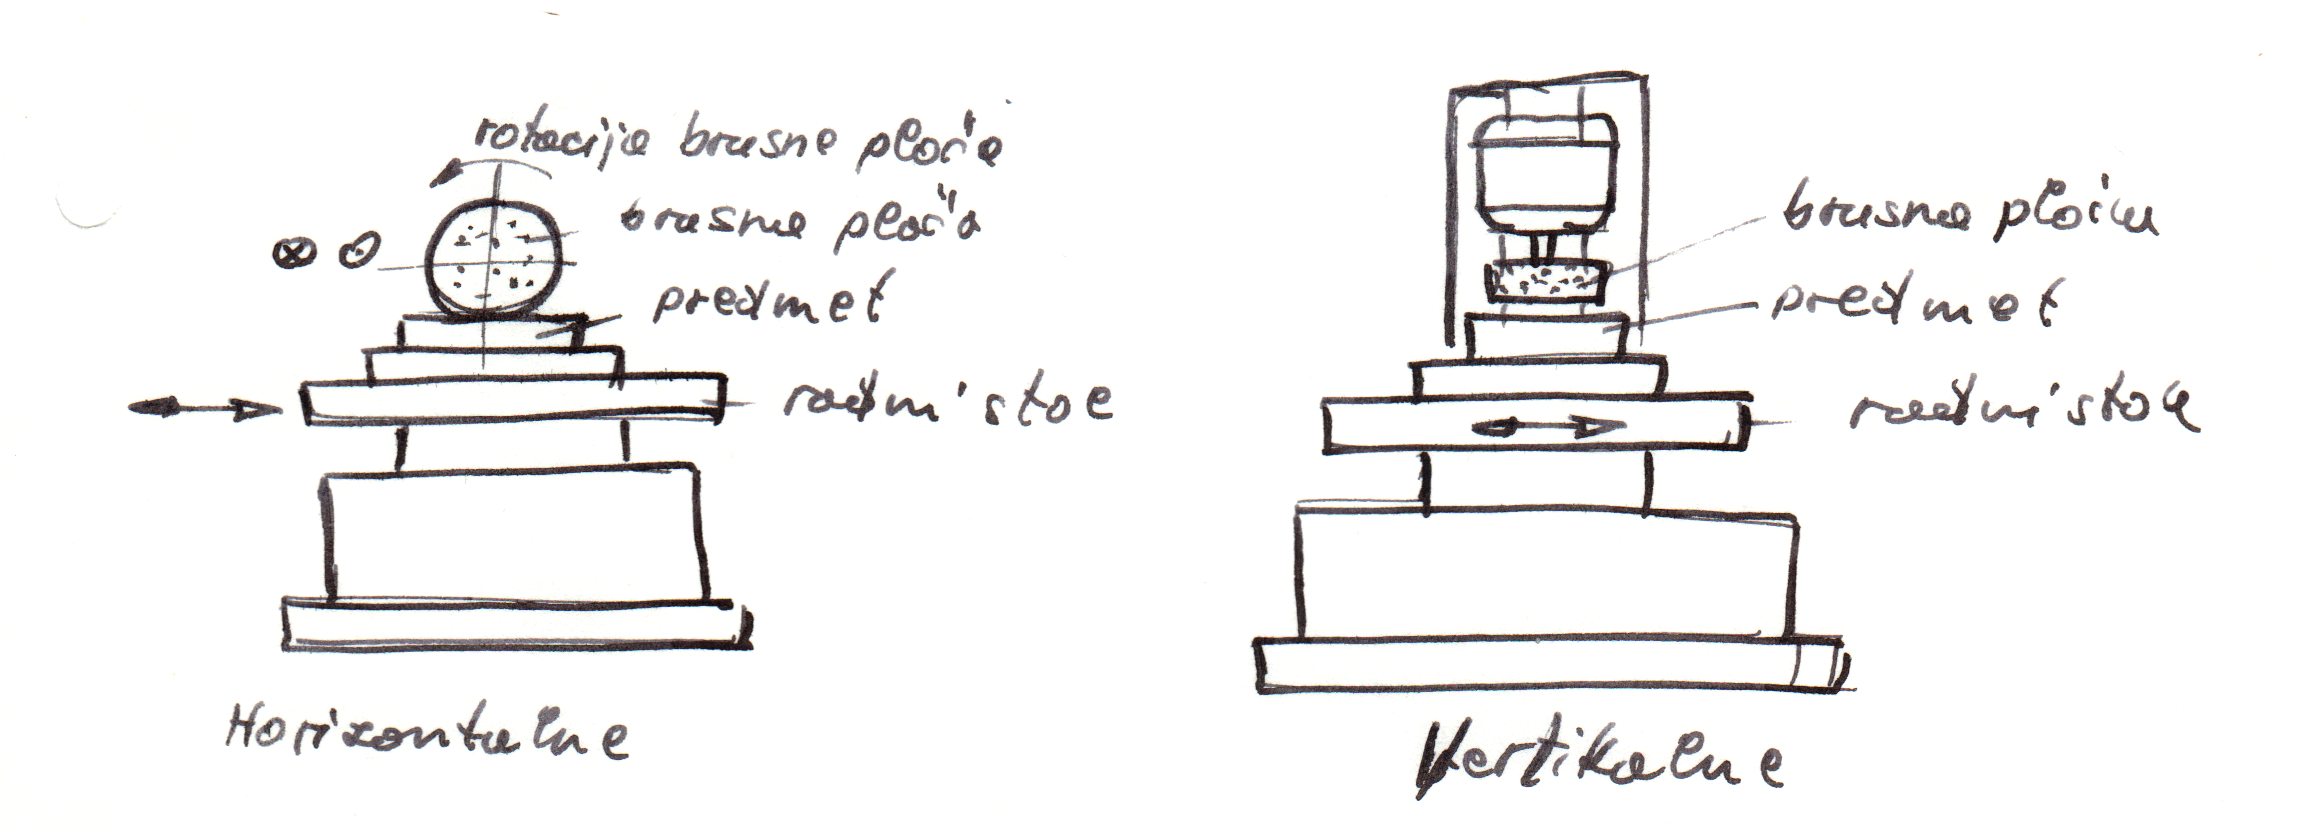
\includegraphics[scale=0.15]{image_28-1.png}
\end{figure}
\FloatBarrier
Kod vertikalnih brusilica razlikujemo dvije mogućnosti međusobnog dodirivanja predmeta i brusne ploče, točnije čela brusne ploče. Kod vertikalnih brasilica koriste brusne ploče lančastih oblika.
\begin{figure}[!h]
\centering
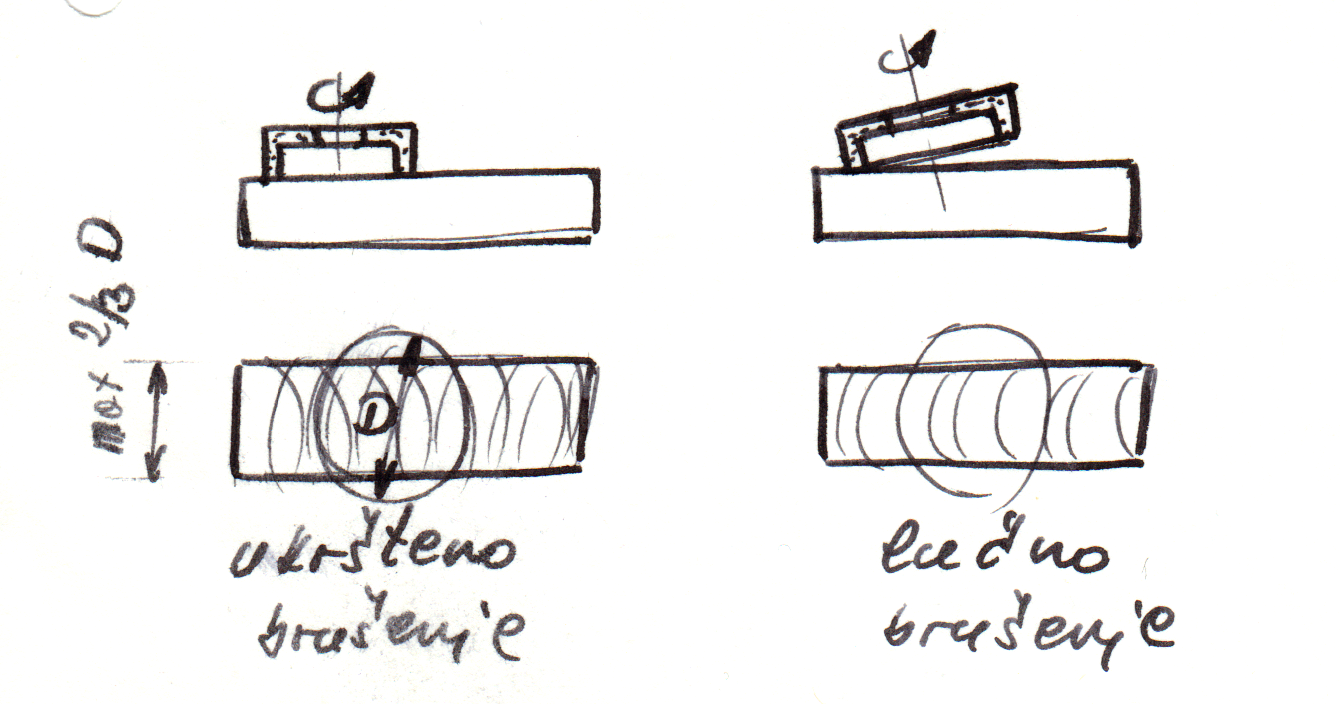
\includegraphics[scale=0.15]{image_28-2.png}
\end{figure}
\FloatBarrier
Za učvrščivanje predmeta na radnom stolu brusilice koriste se isključivo ili elektromagnetskim pločama ili permanentnim magnetnim pločama.\par
Princip rada elektromagnetne ploće je u tome da se jezgra od feritnog materijala, materijala koji se da dobro magnetizirati, magnetizira propuštanjem istosmjerne struje kroz namote. Ti namoti obuhvaćaju niz jezgri koje su međusobno izolirane, a sve zajedno čine ploču. Magnetske silnice, koje se pojavljuju u jezgrama, međusobno zatvaraju preko predmeta i na taj način fiksiraju predmet uz ploću.\par
Nedostatak elektromagnetiziranih ploča za pritezanje je u tome što je za njih potrebna istosmjerna struja, koju dobivamo ili generatorom istosmjerene struje ispravljačima. Osim toga postoji opasnost probijanja električne izolacije među jezgrama zbog korištenja rashladnih sredstava prilikom brušenja, koja su ovdje veoma značajna.\par
Svi ti nedostatci elektromagnetne ploće izbjegnuti su korištenjem ploće za pritezanje s permanentnim magnetima. Princip rada ove ploće je isti kao i kod predhladne, ali ona se sastoji od dviju ploča koje se međusobno daju pomicati i na taj način ostvaruje zatvaranjem magnetskih silnica, jednom kroz gornji presjek a drugi puta kroz predmet. 
\begin{figure}[!h]
\centering
\includegraphics[scale=0.15]{image_29.png}
\end{figure}
\FloatBarrier
\subsection{Strojevi za okrugla brušenja}
Strojevi za okrugla vanjska brušenja slični su tokarilicama. Predmet je upet među šiljke i okreće se, dok brusna ploča zglobno učvršćena i vrši glavno kretanje, rotaciju oko svoje osi. \par
\begin{figure}[!h]
\begin{flushleft}
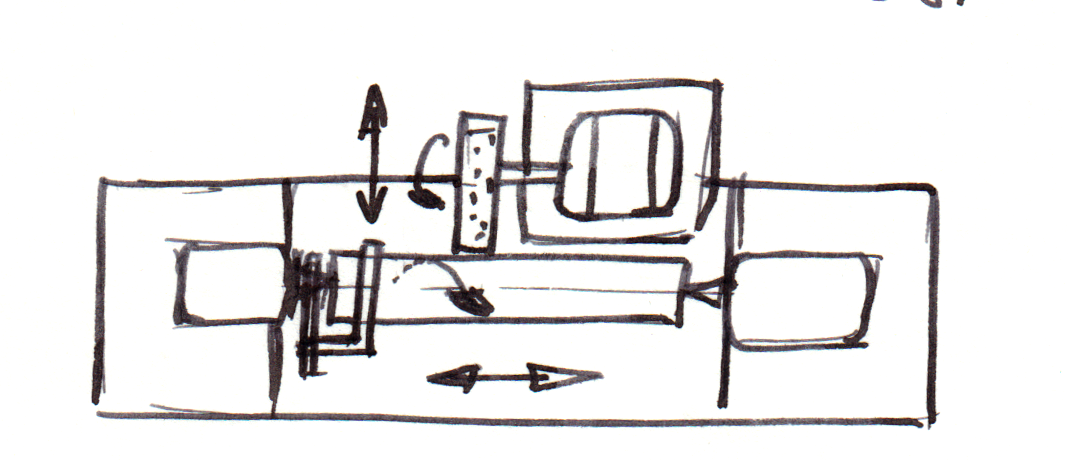
\includegraphics[scale=0.15]{image_30-1.png}
\end{flushleft}
\end{figure}
\FloatBarrier
Razlikujemo dvije mogućnosti
\begin{enumerate}
\item Da brusna ploča sa svojim prigonom vrši i aksijalni pomak duž predmeta. To se koristi za dugačke proizvode da nam radni stol svojim gibanjem nebi zauzeo previše prostora
\item Da se prednost giba uzduž svoje osi zajedno sa stolom na kojem je upet. Takovo riješenje se koristi za izradu malih i kratkih proizvoda.
\end{enumerate}
Poseban način brušenja je \textit{brušenje bez šiljaka} (centerless system). 
\begin{figure}[!h]
\centering
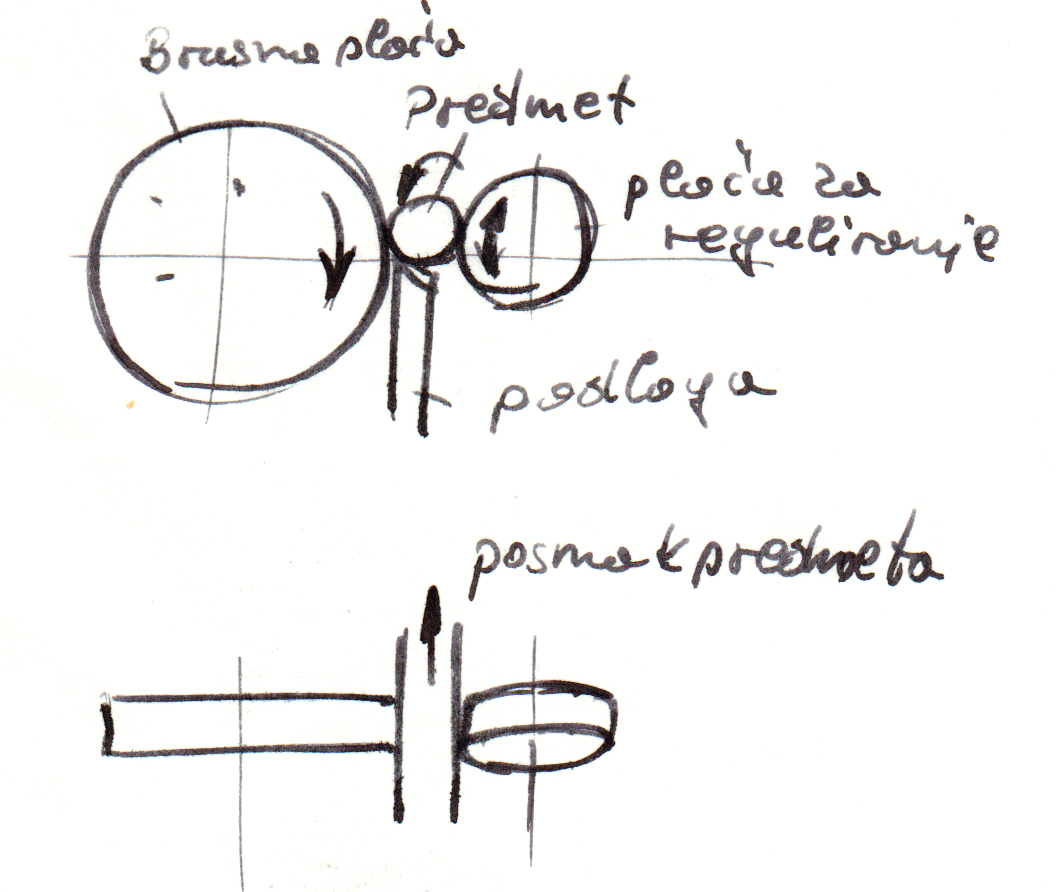
\includegraphics[scale=0.15]{image_30-2.png}
\end{figure}
\FloatBarrier
Predmet leži na podlozi na ploči za regulaciju od koje dobiva rotaciju oko svoje osi. S druge strane predmet dodiruje brusnu ploču koja zbog razlike brzina predmeta i nje same skida strugotinu. Ovisno o veličini nagiba ploče za regulaciju do $5^{\circ}$ dobivamo automatski posmak predmeta. Ovom tehnikom moguće je izrađivati dugačke predmeta, a ujedno je izbjegnuto dugotrajno mukotrpno centriranje. Ovom tehnikom moguće je izrađivati dugačke predmete, a ujedno je izbjegnuto dugotrajno i mukotrpno centriranje. 
\subsection{Brusilice za unutarnja okrugla brušenja}
Brusilice ovog tipa veoma su slične tokarskim strojevima. Predmet učvršćuje u steznu ploču ili amerikaner, a u suportu je učvršćen nosač brusne ploće koji ima vlastiti elektromotor. Predmet se vrti oko svoje osi dok se brusna ploča vrti oko svoje osi ali i tako da dodiruje predmet. Uz glavno kretanje brusna ploča vrši i uzdužno kretanje.
\subsection{Univerzalni strojevi za okrugla brušenja}
Univerzalni brusilicama možemo obrađivati vanjske i unutarnje cilindrične površine. Možemo brusiti i konične površine, ali tako da je predmet upet konično. Kod ovih brusilia koristi se tkz. \textit{planetarni sistem} i to bilo horizontalno bilo vertikalno.
\begin{figure}[!h]
\centering
\includegraphics[scale=0.15]{image_31.png}
\end{figure}
\FloatBarrier
\subsection{Strojevi za brušenje zupčanika}
Iz iskustva znamo da zupčanici imaju dulji vijek trajanja ako im je površina tvrđa i ako su glatko obrađeni. To je dovelo do nastajanja brusilica za zupčanike. Najpoznatiji je princip po MAAGU gdje se to vrši sa dvije brusne ploče. Brusne ploče su postavljene tako da radne površine emitiraju oblik idealne zabne letve. Zupčanik, koji se obrađuje, izvodi translatorna gibanja i na taj način se dobiva dobro sprezanje zupčanika sa \textit{zubnom letvom}. \par 
Na takovim uređajima postoje korekciski instrumenti, koji pomoću servo uređaja dotjeruju položaj brusnih ploča. (Horvat str 499.-500.)
\subsection{Brusilice za brušenje alata}
Postoji čitav niz namjenskih brusilica za razne alate, kao naprimjer npr. glodala, spiralna svrdla, tokarske i blanjačke noževe itd. (Hribar str. 161. i 162.)\par
Kod obrade glodala za izradu zupčanika postoji čitav niz mogućnosti brušenja raznih dijelova oštrica.
\begin{figure}[!h]
\centering
\includegraphics[scale=0.15]{image_32.png}
\end{figure}
\FloatBarrier
\subsection{Specijalne brusilice}
U ovu kategoriju brusilica ubrajamo sve brusilice koje su namjenjene za posebne svrhe npr: brušenje navoja, ventilskih sjedišta ili brusilice koje rade u nešto drugačijim uvijetima od ostalih brusilica. Tu ubrajamo uređaje za:
\begin{itemize}
\item \textbf{Honovanje} - obrada rupa sa čvrsim brusnim sredstvom. Alat je ovdje vođen rupom, koju treba fino obraditi, tj. nije više stroj onaj koji definira položaj alata. Tim postupkom se fino dotjeruju površina i oblik otvora. Hrapavost površine je 0.1-1,5 $\mu m$. (Hribar str. 163)
\item \textbf{Super finiš - mikro honovanje} - to je nešto modificiraniji oblik honovanja, ovdje su glavnom kretanju alata dodate male oscilacije u okomitom pravcu na glavno gibanje. Kod superfiniša se koriste sitnija zrna u alatu nego kod honovanja. (Zdenković 72. str.)
\item \textbf{Lepovanje} - je skidanje strugotine slobodnim kretanjem brusnim zrncima u tekučoj ili tjestastoj smjesi, u kojoj predmet pritisnut u odgovarajući alat čiji se dijelovi raznomjerno okreću. Na taj način se kruta geometrija alata prenosi na izradak. (Hribar 163. str. i Zdenković 75., 76. i 77. str.)
\end{itemize}
\subsection{Brusevi}
Brusna sredstva mogu biti prirodnog ili umjetnog porijekla različitog kemijskog sredstva i razne ali uvijek visoke tvrdoće. Na osnovu toga brusna sredstva možemo podjeliti na:
\begin{enumerate}
\item \textbf{Oksidna sredstva}
\begin{itemize}
\item aliminijski oksid $AR_{2}O_{3} + FE_{2}O_{2}$ koji može biti \textbf{prirodni koruna} ili \textbf{elektro korund - šmirak} tvrdoće do 3000 Hv
\item silicijev oksid $SiO_{2}$ - kremen ili kvarc s tvrdoćom do 1500 Hv.
\item kromov oksid $C_{2}O_{3}$ koristi se kao polirna sredstvo
\item željezni oksid $Fe_{2}O_{3}$ koristi se kao polirna sredstva
\end{itemize}
\item \textbf{Karbidna sredstva}
\begin{itemize}
\item silicijev karbid $SiC$ - karborund dobiven električnom sintezom iz kremena i ugljena tvrdoće 3000 Hv.
\item borni karbid $B_{4}C$ tvrdoće oko 3500 Hv.
\end{itemize}
\end{enumerate}
Za izradu bruseva prvenstveno se koriste elekrokurund za brušenje čelika i žilavih materijala te karborund za brušenje sivog ljeva te tvrdih i krhkih materijala. \par
Za efekt brušenja važna je zrnatost sredstva od kojeg je načinjen brusni kamen. Prema NORTON-ovoj skali, koja označava broj očica na fcoll mreže kroz koju se zrnca siju razlikujemo
\begin{itemize}
\item Vrlo gruba zrna od 3000 - 1700 $\mu m$ ili 8 - 12 rupa
\item Gruba zrna od 170 - 700 $\mu m$ ili 14 - 24 rupa
\item Srednja zrna od 700 -250 $\mu m$ ili 30 -60 rupa
\item Fina zrna od 250 - 100 $\mu m$ ili 70 - 120 rupa
\item Vrlo fina zrna od 100 - 45 $\mu m$ ili 150 - 240 rupa
\item Izvanredno fina zrna od 45 - 20 $\mu m$ ili 280 - 600 rupa
\item Prašinasto od $<$20 - 0,5 $\mu m$ ili 700 na dalje rupa
\end{itemize}
Zrna sitnije od 600 $\mu m$, klasificirano su flotacijom. Da bi zrnca držali na okupom u određenoj formi, međusobno ih povezujemo vezivom. Vezivo ima zadaću da odpusti zatupljeno zrno i dovede novo još nezatupljeno zrno na mjesto rada. Vezivo mora omogućiti i zahtjevima mazanja, odvođenja špene (\textit{pilotine}) i hlađenju koje se ostvaruje raznim sredstvima za uspješnije provođenje procesa brušenja. \par
Prema porijeklu, veziva razlikujemo 
\begin{enumerate}
\item \textbf{Anorganska veziva}
\begin{itemize}
\item keramička veziva - glina tinjac i kvarc, koja su kruta i porona
\item mineralna veziva - vodeno staklo, magneti i silikati, koja su manje čvrsta i tvrđa za fina brušenja.
\end{itemize}
\item \textbf{Organska sredstva}
\begin{itemize}
\item prirodna (vegetativna) sredstva - šelak i razne prirodne smole, žilava i elastična, osjetljiva za zagrijavanje.
\item umjetna veziva - umjetna smola (bakelit), umjetni elastični materijali (elastomeri), žilava i elastična, osjetljiva na zagrijavanje.
\end{itemize}
\end{enumerate}
Po tvrdoći veziva obilježavamo slovima prema oznakama firmi pa ih možemo složiti u 6 grupa:
\begin{itemize}
\item vrlo mekana E,F,G
\item mekana H, I, J, K
\item srednje tvrđa L, M, N, O
\item trda P, Q, R, S
\item vrlo tvrda T, U, V, W
\item izvanredno tvrda X, Y, Z.
\end{itemize}
Po gustoči veziva su svrstana u tri grupe, a to su gusta veziva  (I, II, III), srednje gusta veziva (IV, V, VI) i rahlo veziva (VII, VIII, IX).\par
Oznake brusnih ploča u sebi nose sve veličine interesantne po pitanju izbora brusne ploće i to: veličinu zrna, vrsta zrnaca, tvrdoća i gustina veiva, a svaki proizvođač ima svoju odgovarajuću oznaku uz oblik, koji može biti različit ili uz ravnu ploču.
\begin{table}[!h]
\centering
\begin{tabular}{ll}
38 & broj i vrsta brusnih zrna (elektrokorund, karborund) \\
60 & veličina brusnih zrna                                \\
K  & tvrdoća veziva                                       \\
V  & gustoća veziva                                       \\
Ke & vrsta veziva - keramička, mineralna                 
\end{tabular}
\end{table}
\FloatBarrier
Razlikujemo brusne ploče prema svom obliku i to npr:
\begin{figure}[!h]
\centering
\includegraphics[scale=0.15]{image_33.png}
\end{figure}
\FloatBarrier
Oblikovanje brusnog kamena vrši se u kalupima. Praćenje i odgovarajuću tempreaturu odabire se prema vrsti veziva.\par
Visoka temperatura brusne ploće posebno se testiraju na $40 - 50\%$ većim brzinama od radne i to u vremenu od 3 min. Kod većih ploča osobito je važno dobro balansiranje. Zbog lošeg balansiranja može doći do lomova ploće. Za to je u većini slučaja dovoljno samo statičko balansiranje na posebnim prizamama.
\subsection{Stezanje alata}
Kod pričvršćenja brusnih ploča razlikujemo učvršćenje ploća s malim provrtom i s velikim provrtom.
\begin{figure}[!h]
\centering
\includegraphics[scale=0.15]{image_34.png}
\end{figure}
\FloatBarrier
Kod učvršćenja brusnih ploča veoma je važno da stezne ploče ili prirubnice koje drže bočne stjene brusa budu s mekanim ulošcima. Ti ulošci pri stezanju u radu sprečavaju nepravilno naljepljivanje na strane što bi moglo izazivati iznenadni lom ploče.
\subsection{Režimi obrade}
Obodne bezine brusnog elementa nesmijemo previše povisiti zbog centrifugalnih sila. Kod prevelikih obodnih brzina i brusna ploća djeluje \textit{ko pretvrda} pa ne dobijemo zadovoljavajuće dobru površinu, ploča se brže troši i itd. Zato možemo reći da je potrebno koristiti.
\begin{table}[!h]
\centering
\begin{tabular}{lcc}
Vrsta brušenja          & Brušeni materijal  & Obodna brzina (m/sek) \\
                        & Čelik              & 25                    \\
Kružno i ravno brušenje & Sivi ljev. željezo & 20-25                 \\
                        & Tvrdi metal        & 8                     \\
                        & Legure Al i cinka  & 25                    \\
Oštrenje alata          & Čelik              & 25                    \\
                        & Tvrdi metal        & 12-20                
\end{tabular}
\end{table}
\FloatBarrier
Veličine skidanog sloja se kreću za grubo brušenje (0,02 - 0,05 mm), a za fino brušenje (0,003 - 0,01 mm).
\section{Glodanje}
Glodanje je posebna vrsta površinske obrade sa skidanjem strugotina. Za razliku od tokarenja i blanjanja, glodanje se vrši sa više oštrica, koje naizmjenično dolaze u zahvat. Naizmjenično ulaženje oštrica u zahvat s predmet, prethodnoj oštrici do novog ulaženja u zahvat ostaje slobodno vrijeme, pa se ona uz dobro hlađenje može ohladiti. Takav naizmjenični rad oštrica znatno produžuje vijek trajanja jednog alata za glodanje.\par
Glodala predstavljaju složenu skupinu alata, koja je bogata s oblicima, obzirom na površinu i površine koje obrađuju. Te raspoznajemo:
\begin{itemize}
\item Valjkasto glodalo - za obradu ravih površina koje mogu imati ravne ili kose zube. Kod ravnih zubi glodala promjene sila su znatnije dok kod kosih imamo postepena ulaženja i izlaženja zuba iz zahvata.
\item Valjkasto čeono glodalo - koje uz valjkaste oštrice ima i oštrice na čelu za obradu bočnih površina
\item Pločasto glodalo - s umetnutim zubima, kod kojeg je širina relativno mala spram promjera. Mogu biti brušena za rad s obodnim zubima, a također i za rad s obje čeone površine, a to se naziva pločasto glodalo s ukrštenim zubima
\item Vretenasto glodalo - vrsta čeonog glodala, ali kod njega je promjer znatno manji od njegove dužine za razliku od valjkastog čeonog glodala/ Držak glodala može biti ili cilindričan ili koničan prema Morse propisima.
\item Polukružno udubljeno glodalo - za obradu polukružnih i slični ispupčenih površina.
\item Polukružno ispupčeno glodalo - za obradu polukružnih utora ili utora drugačijih profila.
\item Ugaono glodalo - za izradu utora, rubaca ili utora oblika lastina repa
\item Glodalo za izradu T utora
\item Profilno glodalo - za izradu zubi zupčanika, za izradu spiralnih utora.
\item Glodalo za rezanje navoja - mogu biti izrađene za lijeve i desne navoje.
\item Čeone glave s usađenim noževima - grade se za projere do 250 mm. Tijelo alata je čelik čvrstoće 70 kp/mm$^{2}$, a noževi su od brzoreznog čelika.
\item Dvodjelno valjkasto glodalo - sa suprotno ukošenim zupcima zbog poništenja aksialne sile
\item  Glodala za izradu zupčanika - ima ih nekoliko tipova 
\begin{itemize}
\item tanja rasto glodalo za zupčanike - za Fellov postupak
\item prstasto profilno glodalo za izradu spiralnih zubiju
\item modularno pužna glodala.
\end{itemize}
\end{itemize}
\clearpage
Kod glodala se koriste dvije izvedbe zubiju
\begin{figure}[!h]
\centering
\includegraphics[scale=0.15]{image_35.png}
\end{figure}
\FloatBarrier
Eksperimentalno je dokazano da je veći prednji kut $\gamma$, manja sila rezanja a time i manja snaga elektromotora što daje i manju temperaturu oštrice. Prenost natražno tokarenih glodala je u tome što se kod njih uvijek može postići $\gamma = 0$, dok se kod glodanih zabiju, a $\gamma$ mijenja od brušenja do brušenja.\par
Kod glodanja razlikujemo dva sistema glodanja tj. međusobnog kretanja glodala i predmeta.
\begin{figure}[!h]
\centering
\includegraphics[scale=0.15]{image_36.png}
\end{figure}
\FloatBarrier
Gdje je t dubina glodanja, s$_{z}$ posmak po zubu, s posmak, z promjer zubi glodala, D promjer glodala. \par
Kod protusmjernog glodanja zahvat glodala i predmeta idu od najmanjeg presjeka pa raste do maksimalnog, kod istosmjernog slučaj je obratan, počinjemo s maksimalnim presjekom strugotine a završavamo s minimalnim.\par
Kod  protusmjernog glodanja, dok je još strugotina mala, imamo u stvarnosti klizanje i gnježenje, a to dovodi do povečanja tvrdoće površinskog sloja. To izaziva otežan rad zubaca glodala. Sve to dovodi do jaček trošenja zuba alata, a zbog povećanje tvrdoće i većeg trenja što rezultira veći potrošak radnje rezanja.\par
Kod istosmjernog glodanja, glodalo prvo zahvaća veliki presjek strugotine pa su nastale sile velike. Zbog toga
dolazi do vibracija stola, alat mora biti robusniji, a također i stroj. Zbog međusobnog gibanja predmeta prema glodalu, moraju biti pažljivo izabrani stražnji kutevi. \par
Kod protusmjernog glodanja, glodalo nastoji izbaciti predmet i podići ga od radnog stila. Kod istosmjernog glodanja, glodalo pritiskuje predmet na radni stol. Istosmjerno glodanje oštećuje oštricu glodala manje te dopušta veće ekonomske brzine.\par
U proizvodnji se prilikom obrade primjenjuju oba načina glodanja.\par
Učvršćenje alata na radno vreteno izvodi se na niz veličina. Kod valjkastih glodala s provrtom učvršćenje se provodi na sljedeći način.
\begin{figure}[!h]
\centering
\includegraphics[scale=0.15]{image_37.png}
\end{figure}
\FloatBarrier
Glodajuće glave se učvršćuju bez pomoćnog ležaja je one rade obično čeona glodanja, ali uvijek su svi alati osigurani, kroz radno vreteno, priteznim vijkom.\par
Da bi se izbjegnule prevelike vibracije radnog vretena na kojem je učvršćeno glodalo nastoji se koristiti što je moguće čvršća i jača vretena.
\subsection{Glodalice}
Glodalice možemo svrtati i posebnu grupu alatnih strojeva. Mogučnosti glodalica su raznolike a ujedno i specifične. One mogu obrađivati:
\begin{itemize}
\item ravne površine u vertikalnoj ili horizontalnoj ravnini
\item razne fazonske profine i izradu kojekakvih utora
\item izubljenja alata za skidanje strugotina i zupčanicima
\item razne zavojite površine na vretenima, vijcima, maticama, pužnim kolima i pužnim vijcima
\item razne krivuljaste ploče i šablone
\item najkompliciranije kalupe, ukovnje, gravure, itd.
\end{itemize}
Glodalice je veoma teško svrtati u neki red po bilo kojem karakteru, jer su toliko specifične. Jedna od mogućih podjela je:
\begin{itemize}
\item horizontalne glodalice
\item vertikalne glodalice
\item specijalne glodalice
\end{itemize}
Jedan od najčešćih tipova glodalica je \textbf{univerzalna glodalica} i ona se koristi za obradu ravnih i fazonskih površina, za izradu raznih utora, a pomoću diobene glave mogu se izrađivati ozubljeni alati i čeoni zupčanici.
\begin{figure}[!h]
\centering
\includegraphics[scale=0.15]{image_38.png}
\end{figure}
\FloatBarrier
Brzine automatskih posmaka u horizontalnim ravninama je 20 - 300 mm/min a u vertikanom pravcu 50 - 150 mm/min. Gornji stok se može u horizontalnoj ravnini zakrenuti do 35$^{\circ}$ lijevo ili desno. Ako je to premalo onda koristimo vertikalnu glodalicu.\par
\textbf{Vertikalna glodalica} - za čeonu obradu ravnih površina, za obradu ravnih, kosih i spiralno zavinutih utora, za obradu ravnih s ravnim dnom itd. Ako se na gornji stol postavi rotirajuća ploća, moguće je obrađivati razne koncentrične utore korištenje diobenih glava također dolazi u obzir.\par
Kod ove izvedbe glodalice, radno vreteno je postavljeno vertikalno na radnu površinu stola. Kod vertikalnih glodalica modernije izvedbe ugrađena je i mogućnost zakretanja radnog vretena pod izvjesni kut prema površini stola. To je veoma pogodno za izradu najrazličitijih kosih površina.\par
Uz dva horizontalna posmaka stola, postoje izvedbe, kod kojih je i rotacija radnog stola također automatsko. (Hrabar str. 140.)\par
\textbf{Specijalne glodalice} - je skupina strjeva pretežno namjenjena za specijalne svrhe kao npr:
\begin{itemize}
\item izrada zupčanika a tu je najpoznatija tkz. PFAUTER-glodalica a radi na principu odvaljivanja
\item izradu pužnih kola
\item izradu navoja i pužnih vijaka
za kopiranje i graviranje pomoću šablona i uzoraka itd.
\end{itemize}
U familiju specijalnih glodalica možemo ubrojiti i glodalice s dva ili više radnih vretena, od kojih imamao odmah vertikalno i horizontalno radna vretena za višestranu obradu. (Hrabar str 142. - specijalna glodalica s 4 vretena)\par
Nekoliko puta spominjana je diobena glava za izradu raznih predmeta, pa da se sada upoznamo malo pobliže.
\subsection{Diobene sprave}
Kod izrade čeonih zupčanika za glodalicama za dijeljenje kruga koristimo tkz. \textbf{diobenu glavu}. Nakon svakog pojedinog izrađenog zuba potrebno je predmet zakrenuti za z-ti dio njegovog opsega.\par
Najviše upotrebljavana konstrukcija diobene glave je na principu pužnog prijenosa čiji je prijenosni odnos obično f:40. Za zakretanje ručice, za bilo koji dio od punog kruga koriste se diobene ploče s rupicama, raspodijeljenih u više koncentričnih krugova, a na svakom krugu je drugi broj rupica. Brojevi rupica koj se primjenjuju su 15-16-17-18-19-20-21-21-23-27-29-31-33-37-39-41-43-47-49 dokle ukupno 18 krugova koji se mogu smjestiti na dvije ili tri ploče, koje se mogu međusobno mijenjati.
\begin{table}[]
\centering
\begin{tabular}{ll}
z      & broj zubaca koje treba izraditi \\
i = 40 & prijenos od ručice pužno kolo  
\end{tabular}
\end{table}
\FloatBarrier
Broj okretaja ručice se određuje iz broja zubi i prijenosnog odnosa
\begin{equation}
n_{r} = \frac{i}{z}\:,
\end{equation}
\begin{enumerate}
\item z $\cdot$ 20 zubi -> $\displaystyle{n_{r}}$ = $\displaystyle{\frac{i}{z}}$ = $\displaystyle{\frac{40}{20}}$ = 2 - dva puna okretaja
\item z - 25 zubi -> $n_{r}$ = $\displaystyle{\frac{i}{z}}$ = $\displaystyle{\frac{40}{25}}$ = 1, $\displaystyle{\frac{3}{5}}$ ili jedan okretaj i još $\displaystyle{\frac{3}{5}}$ a to možemo na ploči s 15 rupa dodati još 9 rupa da bi prošli $\displaystyle{\frac{3}{5}}$ kruga
\item z - 110 zubi -> $\displaystyle{\frac{i}{z}}$ = $\displaystyle{\frac{40}{110}}$ = $\displaystyle{\frac{4}{11}}$ = $\displaystyle{\frac{12}{33}}$ što znači da na ploči od 33 rupe moramo odbrojiti po 12 rupa da bi izveli kretanje predmeta za $\displaystyle{\frac{1}{110}}$
\end{enumerate}
Da bi sredili npr. 53, 69, 125, 137 ili drugi broj zubi, nemoguće nam je kod toga toga izraditi taj broj zubiju s unaprijed navedenim diobenim pločama. Kod izrade tih brojeva, koristimo se tkz. \textbf{diferencijalnom metodom dijeljenja}. Princip te metode se sastoji u tome, da se odabere neki bliski x broj, koji se da diobom izvesti. Nastala diferencija, takvim prijelazom na približan broj zubi ostvaruje se ispravljanjem na taj način, da vreteno pužnog kola, za vrijeme diobe, zakreće diobenu ploču, preko posebno uključenih zupčanika, da se nadoknadi odgovarajuče diferencije.
\begin{figure}[!h]
\centering
\includegraphics[scale=0.15]{image_39.png}
\end{figure}
\FloatBarrier
\noindent Broj zakreta ručice određuje se
\begin{equation}
n_{r} = \frac{i}{x} = \frac{40}{x}\:.
\end{equation}
A omjer zupčanika koji vrše korekciju diobene ploče je
\begin{equation}
k = \frac{i}{x}(x-z) = \frac{40}{x}(x-z)\:,
\end{equation}
gdje je z stvarni broj zubi, dok je x pomoćni broj zubi. Za $x>z$, izlazi k pozitivan, tada se diobeni ploča za vrijeme okretanja ručice zakreće u istom smjeru u kojem i ručica, a za k negativan diobena ploča se okreće u suprotnom pravcu od smjera zakrtanja ručice.
Primjer za z = 127 zubi, te x = 128 odabrani.
\begin{equation}
n_{x} = \frac{i}{x} = \frac{40}{128} = \frac{5}{16}\:,
\end{equation} 
na kraju od 16 rupa prelazimo na 5
\begin{equation}
k = \frac{z_{1}}{z_{2}} = \frac{40}{128} (128-127) = \frac{40}{128} = \frac{30}{96}
\end{equation}
Za prijenos odobreno zupčanika 30 i 96. Za diobeno dijeljenje se uz diobenu glavu uzimajući garnitura zupčanika i to 24, 24, 28, 28, 30, 32, 39, 40, 44,48, 48, 56, 64, 72, 76, 86, 98, 100, 127.\par
Diferencijalno dijeljenje može se primjeniti samo kod izrade zupčanika i glodala s ravnim zubima. Kod izrade kosih ili spiralnih zubi osovina pužnog kola vezana je uz vretena stola glodalice da se osigura potrebno zakretanje.\par
Raznim kombinacijama možemo izraditi na glodalicama i najkompliciranje izvedbe zupčanika ili kakvih drugih djelova.
\subsection{Režimi obrade}
Kod glodanja, kao osnova za određivanje ekonomskih brzina uzima se količina stisnutog materijala u jedinici vremena.\par
Ekonomskih brzina rezanja ovisi veoma mnogo o složenosti oblika glodala. Što je veća dimenzija glodala, što je oblik kompliciraniji, trebalo bi da glodalo dulje traje između dva brušenja. To trajanje između dva prebrušivanja kreće se u granicama od 1 do 8 sati, tj. korsite se $^{\nu}$60, $^{\nu}$180, $^{\nu}$240, $^{\nu}$480.
Jasno je da se veličina brzine rezanja korigira u ovisnosti od 
\begin{itemize}
\item obrađivanog materijala
\item vrste obrade tj. kvaliteti površine
\item kvaliteti glodala
\end{itemize}
Sve to utječe i na izbor i veličinu posmaka.
\begin{table}[!h]
\centering
\begin{tabular}{|c|c|c|c|c|}
\hline
\multirow{3}{*}{Odabrani materijal} & \multicolumn{4}{c|}{Brzina rezanja u m/min}                              \\ \cline{2-5} 
                                    & \multicolumn{2}{c|}{Brzorezni čelik} & \multicolumn{2}{c|}{Tvrdi metali} \\ \cline{2-5} 
                                    & grubo             & fino             & grubo           & fino            \\ \hline
Obrađeni Če i Če-lijev              & 8-15              & 15-25            & 30-80           & 90-100          \\ \hline
Lijevano željezo                    & 8-12              & 12-20            & 50-80           & 80-100          \\ \hline
Bronca i mjed                       & 20-25             & 30-50            & 90-120          & do 300          \\ \hline
Laki metali                         & 400-1200          & 600-1500         & -               & -               \\ \hline
\end{tabular}
\end{table}
\FloatBarrier
Dubina rezanja kreće se od 1-15 mm a posmaci od 0,02-0,25 mm/zubu.
\section{Kovanje}
Kovanje je obrada metala bez skidanja strugotina. Može se vršiti u toplom ili hladnom stanju, ovisno o vrsti materijala. Princip kovanja je da se materijal podvrgne djelovanju vanjskih sila koje u njemu izazovu naprezanja između granice elastičnosti i granice loma. Kada na predmet djeluje neka sila, i kada ona prestane djelovati, predmet zadrži novi oblik.\par
Kod kovanja nam se pojavljuju sile koje možemo proanalizirati na sljedeći način. Udarimo čekićem mase G [kg] koji ima brzinu v [m/s] po predmetu, u momentu sraza čekić koji ima kinetičku energiju
\begin{figure}[!h]
\centering
\includegraphics[scale=0.15]{image_40-1.png}
\end{figure}
\FloatBarrier
\begin{equation}
\frac{m\cdot v^{2}}{2} = \frac{G\cdot v^{2}}{2 \cdot g}\:,
\end{equation}
i na nju predaje na izvršenje deformacije, tj. kinetička se energija pretvara u rad. Pod  djelovanjem sile P dolazi do popuštanja predmeta, koji se zbog toga smanji. Dakle sila P je prešla put S a to je upravo radnja izazvana kinetičkom energijom čekića pa možemo zapisati
\begin{equation}
\frac{m\cdot v^{2}}{2 \cdot g} = P\cdot S\:.
\end{equation}
Sva konetička energija se ne pretvori u izvršenje radnje deformiranja. Jedan dio se gubi zbog popuštanja podloge i čekića (bata) dok se drugi dio gubi ne savladavanje elastičnih sila. Zbog toga se kao  stupanj djelovanja bata uzima 
\begin{equation}
\eta = \frac{G'}{G + G_{1}}\:.
\end{equation}
Obično se uzima da je težina nakovnja 10 do 20 puta veća od težine čekića a kroz to se dobia $\eta = 0,91-0,75$.\par 
Jedan jaki udarac monogo je efikasniji od mnogo manjih a to se odma vidi kada djelujemo na predmet istih dimenzija jednom s batom a drugi puta s mnogo udaraca.
\begin{figure}[!h]
\centering
\includegraphics[scale=0.15]{image_40.png}
\end{figure}
\FloatBarrier
Potrebna sila za obrikovanje, zavisi od veličine tlačne površine F, čvrstoći materijala $\sigma$ i iskustvenom koeficijentu $\phi$. Što nam daje izraz
\begin{equation}
p = F\cdot \sigma \cdot \phi \:,
\end{equation}
gdje $\phi$ ide do 10 kod udarnog djelovanja čekićem a $\phi = 2 - 1,4$ kod polakog pritiskivanja (prešanja). Za obradu predmeta u ukovnju uzet ćemo dvostruke vrijednosti koeficijenta $\phi$.\par 
Želimo li neki veliki predmet obraditi kovanjem, primjenom ručnih alata i čekića to je nemoguće, jer rukom možemo proizvesti samo manje neznatne sile. Za kovanje predmeta teških nekoliko tona, moramo koristiti mehaničke naprave i strojeve. Te uređaje možemo podjeliti na:
\begin{itemize}
\item \textbf{mehaničke čekiće} - kod kojih udarce stvaraju maljevi i
\item \textbf{mehaničke preše za kovanje} - kod kojih se putem hidraulike stvraju sila. Kod toga mi vršimo deformacije više gnječenjem nego udaranjem.
\end{itemize}
\par
\textbf{Mehaničke čekiće} koji mogu imati transmisijski pogon, zatim parni ili zračni pogon, električni pogon itd. možemo dalje podijeliti.
\begin{enumerate}
\item Batovi s kosim udarnim plohama - koji su obično učvršćeni na polugi i emitiranju ručno udaranje.
\item Batovi s paralelnim udarnim plohama koji se mogu dalje podijeliti na 
\begin{itemize}
\item udarni batovi - kod kojih se malj diže a zatim pada vlastitom težinom na predmet koji se obrađuje kovanjem
\item mehanički čekići - koji rade pomoću jake opruge
\item mehanički čekići - koji rade pomoću komprimiranog zraka
\item mehaniči čekići koji rade parom.
\end{itemize}
\item Preše za kovanje možemo međusobno podijeliti na 
\begin{itemize}
\item Udarne preše - a to su one koje imaju neposredan pogon. U tu grupu ubrajamo vretenaste ploče koje mogu biti ručne i frikcione, ekscentar preče te strojevi za kovanje uže namjene
\item Preše s posrednim pogonom - hidrauličkim pogonom.
\end{itemize}
\end{enumerate}
\subsection{Glavne kovačke operacije}
Komad koji želimo obraditi kovanjem, prvo zagrijavamo na temperaturu kovanja. Nakon zagrijavanja očistimo ga od okuine, zahvatimo klještima, stavimo na nakovanj i onda kujemo. Kovanje mogu izvoditi i više ljudi s time da u određenom ritmu udaraju jedan za drugim po predmetu. Kod kovanja većih predmeta koriste se mehanički uređaj (čekići i preše). Masovna proizvodnja kovanih predmeta izvodi se u ukovnjima u na naročitim kovačkim strojevima.\par
Kod kovanja razlikujemo nekoliko glavnih operacija:
\begin{itemize}
\item \textbf{Iskivanje} je najobičniji kovački posao, kojim se kovani predmet stanji, rastrgne, iskuje ili raširi. Kod tog kovanja komad se istovremeno stanji i rastegne po dužini i širini. U tu grupu obrade spada i kucanje posuda.
\begin{figure}[!h]
\centering
\includegraphics[scale=0.15]{image_41-1.png}
\end{figure}
\FloatBarrier
\item \textbf{Sabijanje} je postupak obradom izkivanja. To je nagomilavanje materijala na jednom mjestu, koje je prethodno zagrijemo. To je udaranje materijala u u zdužnom smjeru. To je veoma skup i neprikladan postupak pa ga se nastoji izbjeći.
\item \textbf{Savijanje} - ako se neka šipka savija, na tom mjestu nastupit će suženje i smanjenje presjeka, Zbog toga se šipke koje savijamo prvo sabiju a zatim saviju, i ovdje se savijanje može obavljati oko nekog okruglog profila, a izvodi se ručno kod tanjih šipki.
\item \textbf{Odsjecanje} se vrši ili čekićem u obliku dljeta ili trokutastim alatima pogodnim za tu vrstu kovanja.
\begin{figure}[!h]
\centering
\includegraphics[scale=0.15]{image_42.png}
\end{figure}
\FloatBarrier
\item \textbf{Probijanje} se vrši pomoću probijača. Prvo se s jedne strane probijačem napravi rupa do dubine 2/3 od debljine materijala koju probijamo. Zatim se predmet okene i preostali dio materijala se izbije. Za velike rupe to se izvodi odgovarajućim komadom.
\item \textbf{Sukanje} naziva se još i uvijanje. Komad se zagrije na mjesto koje želimo zakrenuti, učvrstimo ga u škripac i zakrenemo za željeni kut.
\item \textbf{Zavarivanje} je postupak kojim se mogu spajati materijali s veoma malo sumpora a nešto više mangana. Prije zavarivanja, dijelovi koji se žele zavariti oripreme se u određeni najpogodniji oblik, zatim se zagriju za cca 1200$^{\circ}$ brzo približe, pospu dezoksidantom i vještim udarcima zavare.
\item \textbf{Natiskivanje} je navlačenje prstenova na osovine. Prsten se agrije na visoku temperaturu dase može bez velikih problema navući na osovinu. Nakon hlađenja ostvaren je željeni čvrsti spoj.
\item \textbf{Stično svarivanje} mora predhoditi proces zadebljanja krajeva. Nakon zagdijavanja  i stičnog spoja obavezo moramo izvesti prokivanje zavarenog spoja. Ovaj način nam ne garantira kvalitetu i puzdan spoj.
\begin{figure}[!h]
\centering
\includegraphics[scale=0.15]{image_43-1.png}
\end{figure}
\FloatBarrier\item \textbf{Preklopno svarivanje}, kod preklopnog svarivanja spojne dijelove izvedemo na način prikazanom skicom. Ovakav spoj nam daje bolji i pouzdaniji šav.
\begin{figure}[!h]
\centering
\includegraphics[scale=0.15]{image_43-2.png}
\end{figure}
\FloatBarrier\item \textbf{Obuhvatno svarivanje}, ovaj način spoja primjenjuje se kod svarivanja raznoradnih materijala i kod velikih presjeka.
\begin{figure}[!h]
\centering
\includegraphics[scale=0.15]{image_43-3.png}
\end{figure}
\FloatBarrier\end{itemize}
\subsection{Kovanje u ukovnjima}
Da bi izradili seriju istih komada sa što manjim odstupanjima koristimo se postupkom kovanja u ukovnjima. Ukovnji su vrste kalupa, ali od materijala koji mogu izdržati sile kovanja. Ukovnji se obično rade od lijevanog čelika a za manje komade i manje serije od lijevanog željeza.\par
Veličina šupljine ukovanja je veća za cca 1,2\% a to je zbog stezanja materijala kada se on ohladi s temperaturom okoline. Kad konstrukcija ukovnja treba se voditi računa o višku materijala koji se umeće u kalup. Taj višak materijala treba biti zgodno raspodjeljen i da se pretvori u neku vrstu srha odakle ga je moguće jednostavno odstraniti, a nesmeta izgledu.
\begin{figure}[!h]
\centering
\includegraphics[scale=0.15]{image_44.png}
\end{figure}
\FloatBarrier
Kod kovanja u ukovnjima, predmet se prvo iskuje na približan oblik, a zatim se u ukovnju izvrši konačno što manje vrijeme, pa se zbog toga u neke ukovnje ugrađuju izbacivači. Ako bi predmet zaostao dulje vrijeme u kalupu, zbog prijelaza topline s predmeta na stijene kalupa došlo bi do otkaljivanja površine kalupa. (primjeri - horvat I str. 561. - 565.)
\subsubsection{Tempreture kovanja}
Temperature kovanja ovise o vrsti materijala i njegovom sastavu i o načinu na koji se kuje, da li je to komplicirani predmet ili ne, te o opremi s kojim kovanje se vršilo. Najpovoljnije temperature kovanja kreću se u granicama za mekani čelik 900 - 1300$^{\circ}$C, čelik do 0,3$\%$C 870 - 1150$^{\circ}$C, niskolegirani konst. čelik 830 - 1070$^{\circ}$C, nelegirani alatni čelici 770 - 920$^{\circ}$C, bakar 700 - 960$^{\circ}$C, aluminij 200 - 500$^{\circ}$C.
\clearpage
\section{Izvlačenje}
Izvlačenje, kao metoda obrade materijala, spada u grupu obrada bez skidanja struganja. Materijali, koje obrađujemo proživaljavaju plastične deformacije, ali nesmiju doći u područje loma. Oni moraju biti veoma žilavi. U te materijale spadaju čelici s malo ugljika, a osobito limovi koji su  predviđeni upravo za duboka izvlačenja. Limovi za duboko izvlačenje termički su obrađena a to nazivamo dekapiranjem. Postoje limovi koji su jednom, dvaput pa čak i četiri puta dekapirani. Ovi posljednji su namjenjeni za najkompliciranija izvlačenja. Materijali za izvlačenje su još limovi Cu i Al. Prema JUS limovi za izvlačenje nose oznake (Č.0145 P2 - do Č.0148 P4)\par  
Najstariji način izvlačenja bilo je formiranje posuđa od Cu-lima \textbf{kuckanjem}. Izrađivali su se najrazličitiji predmeti, a danas je ta metoda, koju zahtjeva industrijska proizvodnja, je \textbf{izvlačenje}. Postupak izvlačenja zasniva se na činjenici, da materijal podaje kada ga se optereti iznad granice elastičnosti. Neki predmet je kuckanjem mogao dobiti nakon dugotrajnog i strpljivog rada a s ovim postupkom moguće je to isto izvesti, ako ne u jednom onda u nekoliko radnih operacija. \par
\begin{figure}[!h]
\centering
\includegraphics[scale=0.15]{image_45-1.png}
\end{figure}
\FloatBarrier
Čitav uređaj za izvlačenje učvršćen je na radnom stolu preše, koja je namjenjena za duboka izvlačenja. To mogu biti hidrauličke ili ekscentar preše. Uređaj se sastoji od žiga i matice koji određuju oblik predmeta. U sklopu postoji i pridržač lima koji sprečava klizanje lima i time osigurava plastičnu deformaciju predmeta. \par
Postupak izvlačenja teče u određenim koracima a ovu su otprilike ovakvi:
\begin{itemize}
\item izrezivanje platine iz koje se najerava raditi predmet
\item izrada prikojene platine, to dolazi u obzir ako želimo izbječi velike zaostatke materijala na rubovima, recimo četvrtastih posuda
\begin{figure}[!h]
\centering
\includegraphics[scale=0.15]{image_45-2.png}
\end{figure}
\FloatBarrier
\item višestepeno izvlačenje, jer odnos smanjenja promjera platine i nastale kolote nesmije biti manji od 0,48
\item nakon konačnog izvlačenja moramo rubove posude obrezati da doijemo željeni oblik, koji može biti ko smije dalje obrađivati.
\end{itemize}
Ako se izvlače posebno duboke posude, potrebno je međufazno poluproizvod izžariti da se odstrani krtost nastala višekratnom deformacijom.\par
Želimo li predmet kruškolikog oblika, nemožemo to izvesti metalnim žigom. Kod toga se koristimo, unaprijed formiranom matricom, a žig je modificiran, a tečenje izvodimo gumom, tekućinom ili čeličnim kuglicama. Pod djelovanjem vanjske, pomoćno sredstvo zauzima unutarnje konture matrice i na taj način formira oblik. Nakon prestanka djelovanja, moguće je izvući i izvaditi to sredstvo iz formirane posude. \par
Primjena dugokog izvlačenja u industrijske svrhe je u današnje doba sve značajnija. Dolazi u obzir u svim granama metaloprerađivačke industrije, Iako je lim za duboka izvlačenja znatnije skuplji, princip rebara veoma efikasno ukrutiti da je čitav proizvod jeftiniji.\par
U našem poduzeću se duboko izvlačenje koristi:
\begin{itemize}
\item za izradu kalota električnih grijača vode, limenih djelova pegli, električnih lonaca itd. u tvornici u Samoboru
\item za izradu dijelova štednjaka, ugostiteljske opreme, izradu sudopera od nehrđajučeg čelika na Žitnjaku
\item za izradu dna hidrofora u Samoboru
\item u proizvodnji dijelova frižidera u Bitoli itd.
\end{itemize}
\clearpage
\section{Valjanje}
Valjanje je način oblikovanja, koji se temelji na plastičnoj deformaciji materijala. Valjanje za izradu u hladnom stanju a također i  u toplom, gnječenom stanju.\par
Valjanje je neprekinuti postupak za smanjivanje presjeka i ujedno produljenje komada koji formiramo. U užem smislu, valjanje je oblikovanje usijanog komada, prolazom između dva valjka, koji su večinom horizontalni, a koji se okreću u suprotnom smjeru. Razmotrimo sile koje se javjaju kod valjanja.\par
\begin{figure}[!h]
\centering
\includegraphics[scale=0.15]{image_47.png}
\end{figure}
\FloatBarrier
Sila N, je sila pritiska nastala zbog deformacije predmeta. Tu silu možemo podjeliti na horizontalnu silu u vertikalnom smjeru. Vertikalna sila pritiska, koju moraju prenositi ležaji valjka dok horizontalna sila trenja $\mu N cos \alpha$. Da bi se proces valjanja odvijao noramlno sila trenja mora biti veća od sile koja želi predmet izbaciti nazad te možemo postaviti jednadžbu.
\begin{equation}
\mu N\cdot cos \alpha > N sin \alpha -> \mu > tg \alpha\:,
\end{equation} 
ako za $\mu = tg\rho$ to se naziva kut trenja uvedemo u jednađbu izlazi daje $\rho>\alpha$ tj. da je kut trenja veći od ulaznog kuta $\alpha$.\par
Kod valjanja se omjer h i h$_{1}$ nesmije prekoračiti pa on izgleda ovako
\begin{equation}
h_{1}=0,9 - 0,6 h\:.
\end{equation}
\clearpage
\section{Savijanje}
\subsection{Savijanje limova}
U svakodnevnom životu susrećemo se s najraznovrsnije svinutim konturama od lima. Tu spadaju svi mogući oblici počevši od okruglih do najkompliciranih fazonskih savijanja. \par
Ploča lima možemo okruglo saviti na dva najjednsotavnija načina, koji se temelje na principu valjaka.
\begin{enumerate}
\item \textbf{Savijanje s tri valjaka} \\
Kod ovog načina savijanja imamo tri valjka koji rotiraju oko svoje uzdužne osi i omogučuju prolaz lima između njih. Ako gornji valjak utisnemo prema dolje dobit ćemo zakrivljenu površinu. Minimalni promjer cilindra diktira promjerom gornjeg valjka. Veliki nedostatak ovog sistema je u tome što se rubovi, tj. početak i kraj moraju predsaviti da bi se dobila sila što bolja cilindrična ploha
\begin{figure}[!h]
\centering
\includegraphics[scale=0.15]{image_48-1.png}
\end{figure}
\FloatBarrier
\item \textbf{Savijanje s 4 ili više valjaka} \\
Kod ovog načina savijanja izbjegnut je nedostatak presvijanja krajeva. Pomoćni bočni valjci omogučavaju savijanje cilindrične plohe bez predsavijanja to je velika prednost. Istina da su ovakvi strojevi nešto komliciraniji i skuplji ali svojim prednostima to pokrivaju.
\begin{figure}[!h]
\centering
\includegraphics[scale=0.15]{image_48-2.png}
\end{figure}
\FloatBarrier
\end{enumerate}
Da bi ploću rubno savili do nekog kuta, danas su još u primjeni dva načina. Prvi način je veoma star ali još uvijek veoma efikasan.
\begin{figure}[!h]
\centering
\includegraphics[scale=0.15]{image_48-3.png}
\end{figure}
\FloatBarrier
Naime, radi se ovdje da se lim stegne u dvije čeljusti i zatim se sa zakretnom gredom izvrši savijanje do željenog kuta. Tom metodom se ručno mogu savijati razi limovi obojenih metala. Nedostatak ove metode je u tome što nemožemo izvršiti savijanje nekoliko rubova blizu jedan drugome. Da bi iz lima savili neko profil, možda i zatvorenog oblika, koristimo se tkz. \textbf{abkant prešama}. To su preše posebnog oblka, kod kojih se u gornji pokretni dio mogu ugraditi alati - tkz. noževi i pomoću njih izvodimo savijanje. Uz nož na stol preše učvršćuje se prizma, kao drugi dio alata za formiranje. 
\begin{figure}[!h]
\centering
\includegraphics[scale=0.15]{image_49-1.png}
\end{figure}
\FloatBarrier
Dužina tih noževa je različita a kreće se i do reda veličine 8 m. O snazi preše ovise kako debeli limovi se mogu saviti. Rad s abkant prešom je jednostavan i veoma produktivan pa se sada one sve više i više koriste.\par
Da bi se profilno savili ploču lima, kod koje ima više veoma plitkih oblika možemo umjesto veoma skupog pripusivanja žiga u matricu, koristiti samo matricu, a umjesto žiga uzimamo odgovoarajuću tvrdu gumu. Pod djelovanjem sile prešanja guma će djelomično formulirati lim koji je stisnut između gume i matrice.
\begin{figure}[!h]
\centering
\includegraphics[scale=0.15]{image_49-2.png}
\end{figure}
\FloatBarrier
Kadkad se na taj način u tvornici na Žitnjaku izrađuju radne ploče za kuhanje a postupak se naziva Tohr-metal koji ima instaliranu prešu snage 5000 t.
\subsubsection{Savijanje punih šiki i profila}
Savijanje punih šipki, koje mogu biti okrugle, pravokutne ili nekog drugog oblika moguće je izvesti na nama već poznatim strojevima za savijanje limova. Mogu se korstiti strojevi s tri ili četiti valjka. Za pravokutne i kvadratne profile savijanje se izvodi na ravnim dijelovima valjka, dok za profilno formirane šipke i profile trebamo imati odgovarajuće kanale da bi ih mogli saviti.\par
Ako se radi o čestom savijanju profila, postoje uređaji namjenjeni isključivo za tu vrstu savijanja. Princip rada je obet putem triju pokretnih valjaka koji imaju najrazličitije kanale, za različite profile. Postavljeni su okomito na površinu poda ili vertikalno.
\begin{figure}[!h]
\centering
\includegraphics[scale=0.12]{image_49-3.png}
\end{figure}
\FloatBarrier
\subsubsection*{Primjer}
Redosljed operacija kod savianja profila.
\begin{figure}[!h]
\centering
\includegraphics[scale=0.15]{image_50.png}
\end{figure}
\FloatBarrier
\clearpage
\begin{figure}[!h]
\centering
\includegraphics[scale=0.14]{image_51-1.png}
\end{figure}
\FloatBarrier
\subsubsection{Savijanje cijevi}
Savijanje cijevi zahtjeva posebnu tehnologiju i to zbog deformacije cijevi na mjestima savijanja. To dolazi kod savijanja cijevi na manjem radijusu, kod malih promjera, dok je to problem kod svih cijevi iznad 50 mm promjera. Da bi se izbjegle deformacije cijevi na mjestima savijanja potrebno je to spriječiti pomoćnim sredstvima. Najjednostavniji način je ispunjavanje cijevi nestlačivim sredsvom, koje će zadržati puni profil cijevi. Za to se koristi, kod manjih cijevi pijesak. Pijesak se naspe u cijev i sa obje strane dobro začepi, zatim se izvrši savijanje bilo ručno bilo u nekom uređaju. \par
Kod savijanja cijevi večeg promjera, umijeto pijeska koriste se druge tehnike.
\begin{figure}[!h]
\centering
\includegraphics[scale=0.14]{image_51-2.png}
\end{figure}
\FloatBarrier
Pomoću podatljivih elemenata vezanih jedan za drugim a to mogu biti čelične kuglice ili neki drugi sferni oblici koji se savijaju zajedno sa cijevima. Kod savijanja plašteva cilindara mogu se pojaviti greške i to:
\begin{enumerate}
\item Krajevi nisu predsaviti na potreban radius, nego mogu zaostati ravni. Zbog toga je potrebno koji puta, ako je potreban točan oblik saviti čitav cilindar preklopna, pa preklop odrezati i na taj način dobiti čisti krug.
\begin{figure}[!h]
\centering
\includegraphics[scale=0.1]{image_52-1.png}
\end{figure}
\FloatBarrier
\item Može se dogoditi da se cilindar, zbog unutarnjih naprezanja lima i različite debljine lima spiralno savije. Ovakvu grešku ispravljamo pomoću posebno konstruiranih sprava, koje nam pri sastavljanju tu grešku korigiraju.
\begin{figure}[!h]
\centering
\includegraphics[scale=0.1]{image_52-2.png}
\end{figure}
\FloatBarrier
\item Svaki predmet bilo kakve obrade ne zaostane uvijek u predviđenom položaju. To se događa također s cilindrično savijenim plaštevima. Kod toga je potrebno kod prihvatnog varenja uzdužnog šava osiguratu optimalni razmak už čitavog vara. Za takvo održavanje koriste se specijalne spravice - naprave s kojima možemo to  održavati.
\begin{figure}[!h]
\centering
\includegraphics[scale=0.1]{image_52-3.png}
\end{figure}
\FloatBarrier
\end{enumerate}
\clearpage
\section{Rezanje}
Odsjecanje materijala razdvajanjem, bez skidanja strugotina, spada u područje obrade, koje se može vršiti noževim raznih oblika, na specijalnim mašinama za odsjecanje (škarama) ili specijalnim alatom na prešama. Pod djelovanjem vanjskih sila pogonskog mehanizma u matrijalu se stvaraju naprezanja koja prelaze čvrstoću materijala, zbog čega dolazi do razdvajanja materijala. \par
Kod odrezivanja, razlikujemo tri faze razdvajanja materijala:
\begin{enumerate}
\item Faza elastične deformacije, kada deformacija nastala pod djelovanjem sile F, nakon prestanka iste nestaje
\begin{figure}[!h]
\centering
\includegraphics[scale=0.15]{image_53-1.png}
\end{figure}
\FloatBarrier
\item Faza plastične deformacije, kad se u predmet pojavilo naprezanje veće od glanice popuštanja
\begin{figure}[!h]
\centering
\includegraphics[scale=0.15]{image_53-2.png}
\end{figure}
\FloatBarrier
\item Prekid materijala, kada se u predmetu pojavi naprezanje veće od čvrstoće materijala. 
\begin{figure}[!h]
\centering
\includegraphics[scale=0.15]{image_53-3.png}
\end{figure}
\FloatBarrier
\end{enumerate}
Da bi odredili veličinu sile rezanja proanalizirati ćemo to na noževima koji se kreću paralelno a imaju i paralelne oštrice.
\begin{figure}[!h]
\centering
\includegraphics[scale=0.15]{image_53-4.png}
\end{figure}
\FloatBarrier
Matrijal nam je pravokutnog presjeka širine b i debljine s. Ravnina A-A je ravnina odjsecanja (idealno). U početku procesa rezanja, noževi prodru u površinu predmeta dubinu z. To se naziva i apsolutna dubina prodiranja. Nakon toga dolazimo do procesa smicanja ili samog odrezivanja. Zbog postepenog prodiranja noža u površinu predmeta, sila F se pomalo seli iz ravnina A-A ovisno o veličini $\alpha$ od ravnine odsjecanja i stvara moment $M = F \cdot a$. Zbog nastanka tog momenta, dolazi do naginjanja samog predmta. Naginjanje izaziva nastojanje bočne sile Fr, a ono će rasti tako dugo dok se moment sile rezanje ne izjednaći s momentom bočne silepa će ravnoteža biti uspostavljenja kada će biti $F\cdot a = Fr \cdot c$. Razvojem jednadžbe došlo bi se do približnog rezutata tg$\gamma\approx\frac{z}{2 s}$. Kut $\gamma$ naziva se kut zakreta materijala. Maksimalna vrijednost sile na škarama ovisi o jačini materijala na smicanje i o apsolutnoj dubini prodiranja noža te to izgleda ovako
\begin{equation}
F_{m} = \bigg(\frac{s}{cos\gamma}\tau_{m}\cdot b\bigg)\:[Kp]\:.
\end{equation}
Za paralelene noževe ta formula poprima vrijednost
\begin{equation}
F_{max} = \tau_{m}\cdot b \cdot s\:[Kp]\:.
\end{equation}
Ovako izračunata sila razanja povečava se za 20-40\% zbog:
\begin{itemize}
\item tupljenja reznih ivica noževa
\item eventualnog povečanja zračnosti među noževima
\item neravnomjernsti debljine materijala koji se odsjeca
\item ostalih nedostataka koji se mogu dogodoti u eksploataciji.
\end{itemize}
\begin{equation}
F_{M} = 1,3 F_{max}
\end{equation}
Ukoliko škare nisu opremljene držačem lima, onda se pojavljuje zakretanje materijala, koje izražavamo kutem $\gamma$ a on iznosi $\gamma = 10^{\circ} - 20^{\circ}$ ili bočna sila $F_{t} = (0,18 - 0,36)F$. Kod škara s držačima lima stanje je $\gamma = 5^{\circ}-10^{\circ}$ a $F_{t} = (0,09 - 0,18)F$. Veličina instalirane snage u uređaju za rezanje ovisi o načinu na koji se odsjecanje vrši. Mi razlikujemo više tehnika i načina odrezivanja, koji imaju svaki svojih prednosti i mana a i posebnih namjena. Kao prvi i najpoznatiji su:
\clearpage
\begin{enumerate}
\item Ravni paralelni ili ravni nagnuti noževi
\begin{itemize}
\item Kod paralelnog odsijecanja $\phi = 2-6^{\circ}$
\item Kod kosog odsjecanje $\varphi = 7-12^{\circ}$
\item Kut klina $\beta = 75-85^{\circ}$
\item Stražnji kut $\alpha = 2-3^{\circ}$
\item Prednji kut $\gamma = 3-12^{\circ}$
\item Zračnost među noževima $f=0,05-0,02$ mm 
\end{itemize}
Ovakvi uređaji se koriste za izrezivanje ploča limova u djelove i to samo ravne rezove.
\begin{figure}[!h]
\centering
\includegraphics[scale=0.2]{image_54-1.png}
\end{figure}
\FloatBarrier
\item Kružni noževi s paralelnim horizontalnim osima
\begin{itemize}
\item Kut zahvata $2\varphi<12^{\circ}$
\item Prekrivanje kružih noževa  $u = (0,2-0,3)s$
\item Dimenzije noževa za $s>10$ mm je D = (25-30)s, a h = (50 - 90) mm dok za $s<3$ mm je D = (35 - 50)s, a h = (20 - 25) mm
\end{itemize}
Primjenjuje se za odsjecanje ploča u trake i za izrazivanje kružnih plotina do s = 30 mm.
\begin{figure}[!h]
\centering
\includegraphics[scale=0.2]{image_54-2.png}
\end{figure}
\FloatBarrier
\item Kružni noževi s gornjom horizontalnom i donjom kosom osi
\begin{itemize}
\item Kut nagiba osovine $\epsilon = 30-40^{\circ}$
\item Dimenzije noževa \\
s$<$10 mm, D = 20 s, h = 50 - 80 mm\\
s$<$3 mm, D = 28 s, h = 15 - 20 mm
\end{itemize}
Koriste se za rezanje ploča u trake te za izrezivanje okruglih prstenova do debljine 30 mm.
\begin{figure}[!h]
\centering
\includegraphics[scale=0.2]{image_54-3.png}
\end{figure}
\FloatBarrier
\item Kružni noževi s paralelnim osima ali nagnutim pod 45$^{\circ}$ prema horizontali 
\begin{itemize}
\item Zračnost f$\geqslant$ 0,2s
\item Razmak razrezanih ivica c$\geqslant 0,3$s
\item Dimenzije noževa za $s>10$ mm je D = 12 s, a h = (40 - 60) mm dok za $s<5$ mm je D = 20 s, a h = (10 - 15) mm
\end{itemize}
Koriste se za rezanje traka, platina raznih vrsta i oblika do debljina 20 mm.
\begin{figure}[!h]
\centering
\includegraphics[scale=0.2]{image_55-1.png}
\end{figure}
\FloatBarrier
\item Kružni noževi s paralelnim osima i više oštrica
\begin{itemize}
\item Kut klina $\beta = 90^{\circ}$
\item Dimenzije noževa \\
D = (40 - 125)s\\
h = (12 - 30) mm
\item Zračnost f = (0,1 - 0,2)s
\end{itemize}
Ovaj način rezanja je visokoproduktivan i koristi se za izrezivanje traka a ovisno o stroju može rezati limove do 10 mm.
\begin{figure}[!h]
\centering
\includegraphics[scale=0.2]{image_55-2.png}
\end{figure}
\FloatBarrier
\item Brzo vibrirajući kosi noževi \\
\begin{itemize}
\item Frekvencije vibracije f = 2000 - 25000 min$^{-1}$
\item Prednji kut $\gamma = 6 -7^{\circ}$
\item Nagib noževa $\varphi = 24 - 30 ^{\circ}$
\item Hod noža 2 - 3 mm
\end{itemize}
Koriste se za odsjecanje raznih kontura s radijusm r$_{min}$ = 15 mm, a izrezuje se prema ucrtanju malim do 3 mm debljine.
\begin{figure}[!h]
\centering
\includegraphics[scale=0.2]{image_55-3.png}
\end{figure}
\FloatBarrier
\end{enumerate}
\subsection{Alat za odsjecanje na prešama}
Prednji kut $\gamma = 2 - 3^{\circ}$, a nagib noževa $\phi = 0$. Alat se postavlja na prešu i najčešće se koristi za odsjecanje pojedinih komada iz traka.\par
\begin{figure}[!h]
\centering
\includegraphics[scale=0.2]{image_56-1.png}
\end{figure}
\FloatBarrier
Široka primjena tehnike rezanja je u štancanju. I ovdje se radi o dvijema ošptricama koje se pokoravaju zakonima poznatih škara i noževa na škarama. Već smo razmotrili slučajeve bez zazora između noževa (žiga) i noža (matrice) i slučaja gdje postoji zazot. Kod štancanja se mnogo primjenjuju i alati sa zakošenim reznim ivicama. Za \textbf{prosjecanje} alati izgledaju 
\begin{figure}[!h]
\centering
\includegraphics[scale=0.17]{image_56-2.png}
\end{figure}
\FloatBarrier
Prije pristupanja rezanja nekog lima na odabranom stroju, moramo podesiti sve parametre, koji odgovaraju za najbolji uspjeh operacije rezanja. \par
Nakon određivanja materijala i njegove debljine, potrebno je podesiti alat. To se posebno odnosi na škare s noževima koji se paralelno gibaju, jer ovisno od debljini materijala, varira zazor i kutevi rezanja, zatim položaj graničnika itd.
\subsection{Rezanje profila}
Profile možemo rezati na posebnim uređajima konstuiranim specijalno za te svrhe. U stvarnosti, to su škare, koje u svojim noževima imaju razne otvore, ovisno o profilu koji mogu rezati. Postoje uređaji za rezanje profila veličine $\Psi 100$; I profil 16 itd. U takvim škarama postoje i kratke škare za rezanje manjih rezova lima.\par
Posebna tehnika rezanja koja se sve više danas primjenjuje je tehnika \textbf{tehnika štancanja}. Tom tehnikom se postižu najveće točnosti, a problem je riješen pomoću posebno konstruiranih alata i preša. Takvim postupkom mogu se izrađivati zupčanici, precizni dosjedi itd.
\section{Ljevanje}
Ljevanje je postupak koji se koristi za izradu složenih predmeta. Sve kovine se ne lijevaju jednako dobro. Na kovinu, koji lijevamo postavlja se nekoliko zahtjeva:
\begin{itemize}
\item da je rastavljena kovina dovoljno žitka
\item da dobro ispunja kalup
\item da odljevak nakon hlađenja bude pun i homogen bez šupljina
\end{itemize}
Dobro se daju ljevati: sivo željezo, cink, bronca, olovo i njegove legure dok se teže lijevaju aluminij i čelik. Od svih kovina najviše se lijeva sivo ljevano željezo. \par
Ljevanje je ispunjavanje šupljine žitkom rastaljenom kovinom. Šupljina, obično u pijesku, napravimo pomoću modela. Kovina se nakon lijevanja skrutne, pa se tako dobiva predmet oblika šupljine ili modela.
\begin{figure}[!h]
\centering
\includegraphics[scale=0.15]{image_57.png}
\end{figure}
\FloatBarrier
Osnovni elementi jednog kalupa spremnog za lijevanje. Ovaj kalup izrađen je od pijeska, kao jedne vrste materijala, od kojeg se kalupi uopće rade. Pješćani kalupi su zasada još najekonomičniji za pojedinačno i maloserijsko lijevanje. Uopće uzev, materijala za kalup bi trebao zadovoljiti sljedeće uvijete:
\begin{itemize}
\item da je jeftin i lako nabavljiv
\item da je dovoljno čvrst, da kalup izdrži bar jedno lijevanje i da je otporan na strujanje i tlak kovine kod ljevanja
\item da se iz njega mogu izraditi glatki kalupi s točnim obrisima, što osigurava točan odljevak
\item da je materijal dovoljno porozan da se osigura lako izlaženje plinova koji se javljaju pri ljevanju
\item loš vodić topline, a ujedno i vatrostalan, tj. da se ne zapeče odljev. Kod kolkile je potrebno da bude dobar vodič topline.
\item materijali jezgre pri stezanju materijala moraju omogućiti te promjene dimenzija. 
\end{itemize}
U prirodi nemožemo pronaći takav materijal, pa zbog toga izvodimo kojekakva mješanja da se bar djelomično približimo traženim uvijetima. U tu grupu materijala spadaju pijesak za kalupljenje, masa, ilovača, pijesak za izradu jezgre, materijali za vezanje jezgrovnog pijeska, tvari za prelake, itd.
\subsection{Pijesak za kalupovanje}
Kao što smo već prije naglasili, materijali za izradu kalupa su mješavina raznih prirodnih sastojaka. Tako je pijesak za kalupovanje mješavina kremenih zrnaca i gline s primjesima vapnenca, lapora, željeznog oksida, raznih spojeva kalcija, kalija, metrija i magnezija. Postotak porimjesa u lijevačkom pijesku nesmije prijeci 5 - 7$\%$.\par
\textbf{Kremena zrnca} - (SiO$_{2}$) okrugla su ili oštrobridna, razne veličine, a čine glavni dio pijeska za kalupljenje. Prema veličini zrnaca razlikujemo finozrnati, srednjezrnati, krupnozrnati pijesak.\par
\textbf{Glina} - zadatak je gline da uz $10 - 12\%$ vlage, obavije kremena zrnca tankom kožicom i međusobno ih povezuje. Zbog toga je pijesak plastičan. Ako su zrnca glatka, potrebno je manje gline a kalupi su čvršći. Što su zrnca veća i jednoličnija, lakše propuštaju plinove koji nastaju kod lijevanja. Finozrnatim pijeskom grade se glađi kalupi ali teže propuštaju plinove. Propustljivost pijeska, odnosno kalupa povečava se tkz. bockanjem i sušenjem kalupa.\par
\textbf{Željezni oksid} - o njegovoj količini u pijesaku ovisi boja pijeska, dali će biti žučkasti ili crvenkasti. Inače njega ima u pijesku uvijek. \par 
\textbf{Vapnenac} se također uvijek nalazi u pijesku. On je uvijek stalan, jer pod djelovanjem topline se raspada i stvara CO$_{2}$ (ugljični dioksid) pa se zbog toga smanjuje popustljivost pijeska. Zapravo, stvara se znatno više plinova koje treba kroz pore kalupa odvesti. Po sadržaju ga dijelimo:
\begin{itemize}
\item kremeni pijesak sa do 2$\%$ gline
\item mršav pijesak 2 - 8$\%$ gline
\item polumastan pijesak 8 - 20$\%$ gline
\item mastan pijesak 20 - 30 $\%$ gline
\item vrlomastan pjesak 30 -50 $\%$ gline
\end{itemize}
\subsection{Pijesak za jezgre}
Kao najbolji pijesak za jezgru pokazao se čisti kremeni pijesak a kao vezivo se koristi laneno ulje. Kao materijal jezgre može se koristiti i mršavi lijevački pijesak s manje od 8$\%$ gline. Osim lanenog ulja, kao dodatci za vezivo jezgre koriste se još:
\begin{itemize}
\item biljna ulja - pamukovo, makovo
\item mineralna ulja - destilacijom nafte
\item životinjska ulja - riblje ulje
\item brašnasti dodatci - raženo, krumpirovo brašno, dekstin
\item smolasti dodatci - kolofonij, sulfitna lužina, melasa
\item sada se jezgre sa 15$\%$ cementa.
\end{itemize}
Kod izrade kalupa koriste se još neki zahvati i materijali, da se pospješi sama proizvodnja lijevanih proizvoda.\par
Da se sprijeći zagaranje pijeska na odljevak, potrebno je kalupnu  šupljinu prevuči \textbf{prevlakom}. Kao prevlaka može se koristiti prah drvenog ugljena ili grafička prašina.\par
Kod izrade kalupa javlja se problem lijepljenja pijeska na modele. Da bi to spriječili, prije kalupljenja naprašimo model. Za naprašivanje se koriste drveni uljen u prašini ili likopodij - crvotočina na crnogorici.
\subsection{Podjela lijevačkog pijeska}
Lijevački pijesak za kalupljnje možemo podijeliti na novi, stari i kaluparski pijesak.
\begin{itemize}
\item \textbf{Novi pijesak} - to su u stvarnosti kremena zrnca koja se kopaju u prirodi. U principu se ne korisit nego se njime regenerira i popravlja stari pijesak.
\item \textbf{Stari pijesak} - to je višekratno korištni pijesak za izradu kalupa i u njemu veći dio gline izgori pa je došlo do oštećenja kremena zrna pijeska.
\item \textbf{Kaluparski pijesak} - pravi se miješanjem fino posijane smjese starog pijeska, s 20 - 50$\%$ novog pijeska, uz dodatno 2 - 15 $\%$ praha kamenog ugljena i 5 - 12$\%$  vode. U tu grupu spada i modelno pijesak za popravak kola koji ima približno isti sastav samo što ima sitnija zrna i veše ugljene prašine.
\end{itemize}
\subsection{Pripremanje pijeska za kalupe}
Pijesak se iskopa, nije moguće odmah primjeniti u lijevaonicama. On je suviše vlažan i u komadima, sadrži u sebi trave, korijenja ili većih komada kamenja. Zbog toga se mora sušiti, sijati, drobiti i separirati. Sve su to zahvati koje je potrebno poduzeti s novim pijeskom da bi ga mogli dodati starom za regeneraciju. Stari pijesak treba očistiti od komadića željeza, lijevačkih čavala i ostalih sitnica koje se javljaju pri ljevanju. U manjim lijevaonicama ovo čišćenje izvodi se ručnim sijanjem, dok se kod većih lijevanica upotrebljavaju čitavi sistem uređaja za pripremu pijeska. U tu pripremu spada i mješanje s novim pijeskom.\par
Računa se da treba 4 - 5 tona za 1 tonu odljeva od sivog lijeva. To znači da za takvu proizvodnju treba svaki put 1 tona novog pijeska za 1 tonu odljevka.
\begin{figure}[!h]
\centering
\includegraphics[scale=0.17]{image_58.png}
\end{figure}
\FloatBarrier
Postoji čitav niz raznih izvedbi bilo kojeg od uređaja za pripremu pijeska. Također postoje posebno konstruirani strojevi za pripremu ilovače i ostalih potrepština za lijevaonice. \par
Da bi izradili kalup, prvo je potrebno izraditi model. Model je izrađen obično od jelovine, a može se koristiti i borovina, joha, lipovina, javor, kruška pa i grabovina. Prema nacrtu predmeta modelar izrađuje model koji mora imati određene dimenzije. Zbog stezanja odljevka, kod hlađenja, dimenzije odljevka se mijenjaju. Da to stezanje nebi prešlo određenu granicu dimenzije odljevka, potrebno je model izraditi veći. Veličina nadmjere ovisi o materijalu koji lijevamo i to:\\ 
\\
Ljevano željezo 1$\%$\\
Temper lijev 1,6$\%$\\
Čelični lijev 2$\%$\\
Bijela kovina 0,5$\%$\\
Bronca, crveni lijev, mjed 1,5$\%$\\
Al-legure 1,1 do 1,25$\%$\\
\\
Modeli koji se koriste za vešekratna, npr. strojna, kalupljena izrađuju se od čvršćeg materijala pa i željeza. \par
Da bi se model lakše izvadio iz pijeska, okomite stranice treba izvesi skošenim. Ako konstrukter ne predvidi skošenja, ona se izvode najmanje 1:100. Kod modela je važno i izvođenje zaobljenja koje može slijediti kalupni pijesak, a da se ne zasipa.\par
Kao posebno kod izrade modela mora se voditi računa o dodatku za obradu na plohama koje obrađujemo. Veličina dodatka ovisi o veličini predmeta, materijalu, načinu lijevanja (horizontalno, vodoravno). Veličina dodatka kreće se od 2 - 15 mm.\par
\textbf{Jezgre} su dijelovi kojim se kalupe šupljine u odljevcima. Jezgre imaju na sebi izdanke za postavljanje u određene položaje u kalupu. Ti upornici se stavljaju na mjestima koja nije potrbno obrađivati nakon lijevanja. Jezgre se uvijek moraju sušiti. Time očvrsnu i postanu propusnije.\par
\textbf{Kalupnici} su okviri bez poklopca i dno u kojima se izrađuju kalupu bilo iz pijeska ili nekog drugog materijala za kalupljenje. Veličine kalupnika odabiremo ovisno o veličini predmeta. Kalupnici mogu biti okrugli ili četvrtasti. Kalupnici mogu biti izrađeni od drveta, lijevanog željeza ili čelika, dok se sada koriste kalupnici od lakih slitina. Kalupnici se koriste u parovima, a mogu biti i trodjelni ili četverodjelni, dok se kod serijske proizvodnje i strojnog kalupljenja koriste naročiti kalupnici za kalupljenje "bez kalupnika". To su ustvari rastavni kalupnici na šarkama.\\
Kalupovanje je postupak za izradu kalupa. Kalupovanje je moguće izvesti i ručno i to:
\begin{itemize}
\item podu ljevaonice sistem mekog i tvrdog kreveta. To je kalupljenje koristi za izradu jednostavnijih predmeta, tako da se u poslu lijevaonice nabije pijesak, na odgovarajući način i izradi kalota, izvedi sistem uljevaka i kalup je gotov. Takvo kalupljenje je najjeftinije.
\item u kalupnicima. To je najuobičajeniji način kalupovanja. Proces izrade kalupa sastoji se u nabijanju pijeska u kalupnik i oko modela. Kad se to izvede, model se izvodi, eventualno se umetnu jezgre, dotjeraju se uljevci i odušnici i kalup je spreman za daljnu pripremu prije lijevanja
\item kalupovanje šestarenje - koji se primjenjuje pri izvođenju kalupa za rotacione predmete svih veličina. Tim postupkom se pojeftinjuje čitav odljevak, jer je vrijeme kalupljenja smanjeno, a trebamo posebno skupe i komplicirane modele. Odljevci izrađeni ovakvim postupcima veoma su točni, jer su izrađeni točnim šablonama. Postupak se vrši šestarima. To su okovane daske koje se mogu okretati oko vretena a imaju obris izvodenice rotacionog tijela.
\begin{figure}[!h]
\centering
\includegraphics[scale=0.17]{image_59.png}
\end{figure}
\FloatBarrier
\end{itemize}
Drugi način kalupovanja bio bi strojno kalupovanje koje se može podijeliti na
\begin{itemize}
\item kalupovanje strojevima s ručnim nabijanjem.\\
Proces nabijanja u pijeska u kalupnik ovdje se opet izvadi ručno, ali operacije odizanja kalupa od modela i njegovo prekretanje vrši se mehanički pomoću strojeva. Kod tih strojeva razlikujemo:
\begin{itemize}
\item strojevi za odizanje - ovdje se odiže čitav kalupnik od modela koji je učvršćen na radnoj površini
\item stroj za spuštanje modelne ploće - ovdje se model s modelnom ploćom spušta prema dolje a na radnoj površini ostaje kalupnik.
\item strojevi s prekretanjem modelne ploće. Tim strojevima se kalupnik preokreće i odma spušta na posebna kolica. Taj postupak olakšava rad od prehladnih strojeva, jer olakšava problematično ručno prekretanje, koje u večini slučajeva izaziva oštećenje kalupa.
\item strojeva provlačenja, koriste se kad visokih odljevaka kod kojih nije moguće izraditi nagibe za izvlačenje modela. Ravne stijenke moraju imati i zupčanici i remenice te se kalupovanje izvodi na ovakovim strojevima. Princip rada se sastoji u tome, da se nakon nabijanja pijeska u kalupnik, model polako pomoću stroja izvuće iz kalupa.
\end{itemize}
\item kalupovanje strojevima za mehaničko nabijanje pijeska
\end{itemize}
Dosada opisani postupci kalupljenja bili su sa ručnim nabijanjem pijeska, a modeli su se vadili ili ručno ili pomoću nekog stanja. Da bi se zamijenilo ručno nabijanje pijeska, konstruirani su posebni strojevi, koji pijesak nabijaju mehanički a ujedno se koriste prije spomenuti strojevi za vođenje modela i okretanje kalupnika. Obzirom na način nabijanja razlikujemo:
\begin{itemize}
\item strojevi za nabijanje pijeska prešanjem. Kod prešanja je pijesak jače sabijen na površinu nego na dnu. Zato se prešanje upotrebljava samo za izvođenje plitkih kalupa. Princip prešanja je da se na kalupnik stavi okvir određene visine, za koju se pijesakmože stisnuti prešanjem, bez opasnosti za kalup. Prešanje se izvodi hidrauličkim putem preko čepa koji ulazi u okvir. Kod prešanja razvili su se postupci:
\begin{itemize}
\item jednostranog prešanja
\item dvostranog prešanja
\item višeslojnog prešanja
\item kalupovanje bez kalupa
\end{itemize}
\end{itemize}
\subsubsection{Kalupovanje strojeva za drmanje}
Pijesak se može sabiti i drmanjem, tresenjem. Tim postupkom, čestica iznad svojom vlastitiom težinom inercijom dijeluje na česticu ispod i tako ju sabija. Zbog toga su čestice na donjim dijelovima kalupnika čvršće sabijene od čestica na povvršini. Strojevi rade s do 300 udarana na minuti i sabijaju velike količine pijeska. \par
Čseto se koristi kominiran uređaj za stresenje i prešanje. Na taj način su dobiveni veoma kvalitetni i donekle jednoliko sabijeni kalupi.
\subsubsection{Kalupovanje strojevima za bacanje pijeska}
Bacanje pijeska u kalupnik moguće je izvesti. U struji zraka - tj. smjesa zraka i pijeska se dovodi u kalupnik. Zrak se odvaja, a pijesak sas vojom brzinom nabija oko modela i ispunjava kalupnik.\par
Drugi princip bacanja pijeska izvodi se pomoću rotirajuće žlice u glavi. Svaki okretanjem žlićice zahvati se malo pijeska i bavi u kalupnik. Pošto se žlićica okreće 1200 do 1600 okretaja, dobiva  se kontinuirani mlaz koji vrlo brzo izpunjava kalupnik.\par
Tvrdoća nabijenog pijeska kod ovih uređaja regulira se brzinom kojom pijesak dolazi u kalupnik. Veće brzine daju tvrđe nabijeni pijesak.
\subsection{Kokilno lijevanje}
Ako želimo neku površinu odljevka posebno tvrdu, potrebno nam je odvesti s te površine brzo toplinu. Brzo odvođenje toplinemožemo ostvariti ako taj dio kalupa izradimo od željeza, koje brzo odvodi toplinu. Takovim postupkom uz tvrdu površinu dobivamo razmjerno mekanu sredinu. Takovim postupkom se lijevaju valjci za valjanje željeza, za papir, platno, mlinove itd.
\begin{figure}[!h]
\centering
\includegraphics[scale=0.17]{image_60-1.png}
\end{figure}
\FloatBarrier
\subsection{Centrifugalno lijevanje}
Za lijevanje cijevi iz dužih rotirajućih dijelova koristi se tkz. centrifugalni lijev. Princip je u tome da se tekuće željezo spiralno namota u kalup od željeza, koji se vrti oko horizontale ili vertikalne osi i ujedno udaljuje od mjesta ulijevanja. Zbog centrifugalne sile, željezo je veoma gusto i bez troske. Željezni kalupi se hlade vodom da se osigura stalna temperature. Odljevci se vade u usijanom stanju pa se izžaruju, da se smanji tvrdoča, koja nastaje zbog naglog hlađenja lijevanog materijala. Cijevi proizvedene ovim postupkom čvršće su za 70$\%$ od cijevi ulijevanih u pijesak iz čega proizlazi da mogu biti i tanje. Postoje još specijalizirani centrifugalni lijevovi i to Morov postupak te ljevanje u hladne kolkile.
\begin{figure}[!h]
\centering
\includegraphics[scale=0.17]{image_60-2.png}
\end{figure}
\FloatBarrier
\subsection{Tlačni lijev}
Za velikoserijsku proizvodnju jednolikih predmeta koriste se tlačno lijevanje. Princip tačnog lijevanja je u tome da se rastavljeni materijal pod pritiskom ubrizga u metalni kalup ili kolkilu. Na taj način dobivaju se veoma točni predmeti  i do 0,01 mm, a osim toga mogu se izraditi i narezi i najrazličitijih gravura. \par 
Za tlačno lijevanje se obično koriste materijali s nižim temperatuream taljenja kao nps. Al-slitine, olovne slitine, kositrene slitine, elektron (Mg Al slitine) itd.\par 
Materijal se prvo rastali u posebnim pećima, a pomoću posebe žlićice ili posudice ulijeva se pred klip koji nakon toga izvrši tlačenje. Ovom tehnikom mogu se lijevati predmeti do težine od nekoliko Kp, što je vezano uz snagu stroja za prešanje i pridržavanje alata. Pritiskom klipa na rastaljeni metal, koji ispunjava kalup, ovisno o proiciranoj površini kalupa, javljaju se veoma velike sile, koje mora preuzeti stroj na sebe.
\section{Termička obrada}
Termičkom obradom zovemo procese kod kojih koristimo toplinu za postizanje nekih promjena u materijalima. Razlikujemo dvije vrte termičke obrade i to:
\begin{itemize}
\item Toplinska obrada u užem smislu - kod koje se ne događaju nikakve kemijske promjene u materijalu
\item Toplinska obrada u širem smislu - kod koje se u stanovitom smislu mijenja kemijski sastav materijala, np. cementiranje, nitriranje.
\end{itemize}
Razmotrit ćemo nekoliko važnih termičkih obrada, koje se međusobno nadopunjuju da bi se na koncu dobio željeni rezultat.
\subsection{Normaliziranje}
Nakon obavljenog kovanja, struktura u predmetu koji smo obrađivali veoma su raznolike iz više razloga. Razlike u veličini kristala, zbog nejednolikog zagrijavanja i hlađenja pojednih dijelovakovanog predmeta nedovoljno dijeluju na kaljenje, koje može slijediti kao slijedeća obrada. Da bi izjednačili veličine kristala , koristimo \textbf{normaliziranje}. Predmet zagrijavamo iznad temperature rekristaliziranja i zatim ga hladimo. Obično je to pregrijavanje za cca 30 - 40$^{\circ}$C. Nakon pregrijavanja predmeta, hladimo ga na mirnom zraku. Na taj način postižemo jednoliku veličinu kristala po presjeku predmeta. Jasno da brzina hlađenja definra veličinu kristala što je ono brže kristali su sitniji. \par
Za dobro odabiranje temperatura normaliziranja potrebno je poznavati sastav materijala.
\begin{figure}[!h]
\centering
\includegraphics[scale=0.17]{image_61.png}
\end{figure}
\FloatBarrier
\subsection{Meko žarenje}
Nakon valjana i kovanja, čvrstoća ugljičnih čelika sa sadržajem ugljika 0,6 - 1,4$\%$C kreće se u granicama od 75 - 100 Kp/mm$^{2}$. Kod legiranih čelika to zna biti i više. Da bi se omogućila obrada tako tvrdih površina, potrebno je sniziti čvrtoću, a to se postiže, \textbf{mekim žarenjem}.\par
Meko žarenje je skoro neophodno za čelik s više od 1$\%$ C, jer kod tih čelika ostaje mogućnost da višak ugljika, iznad 1$\%$ ostaje u prvobitnom stanju, tj. nemožemo utijecat na njega. Žarenje ovisi o količini ugljika i o ostalim legirnim dodatcima.\par 
Najstariji postupak žarenja sastoji se u tome da nelegirane čelika zagrijem na cca 700$^{\circ}$C a legirane za 40$^{\circ}$C više. Materijal držimo na toj temperaturi nekoliko sati a nakon toga ga nastojimo što polakše hladiti. Ovim postupkom listići grafita prelaze u kuglice. \par
Drugi postupak žarenja omogućuje kraće vrijeme čitavog procesa. Materijal se grije iznad temperature rekristalizacije, a zatim se hladi brzinom od 15$\%$ do 650$^{\circ}$C a nastavak hlađenja je proizvoljan. I ovdje je otrebno poznavati točan kemijski sastva materijala.\par
Čelici s mnogo Cr i nehrđajuči čelici žare se tako da ih zagrijemo na temperaturu 800 - 850$^{\circ}$C  i zatim ih hladimo brzinom od 10$^{\circ}$/h do 680$^{\circ}$C. Dalje hlađenje ne utiječe na kvalitetu obrade.
\subsection{Izžarivanje}
Izžarivanje je toplinski postupak kojim otklanjamo zaostale napetosti unutar strukture nekog komada. Predmet, koji želimo izžariti, stavljamo u kutiju s koksom ili čeličnom strugotinom, te ga zagrijemo i držimo na temperaturi 500 - 600$^{\circ}$C  tokom dva sata. Hlađenje predmeta izvesti što je moguće sporije. Ovaj postupak je potrebno provesti prije svakog kaljenja, jer nam nakon kaljenja tako obrađenog predmeta zaostaju neznatne deformacije.
\subsection{Kaljenje}
Da bi postigli veću tvrdoću i čvrstoću materijala koristimo se termičkim postupkom kaljenja. Ovim postupkom u stvari dovodimo do rekristalizacije, povišenjem temperature, ali ne dozvoljavamo ponovnu prekristalizaciju, nego, brzim hlađenjem zadržavamo prethodno formirane kristale. Zbog brzog hlađenja, prethodno rekirstalizirani kristali zadržavaju svoj oblik te postaju veći i nepravilni. To povećanje iznosi i do 1$\%$. \par
Kod kaljenja je najvažnije izabrati odgovarajuće sredstvo za hlađenje. Izbor sredstva definira nam tkz. \textbf{martenzitne strukture}. Za odabiranje brizne hlađanja postoje tkz. \textit{C-dijagrami}.
%SLIKAA
Postoji i tkz. kritična brzina, to je brzina koja tangira liniju početka pretvorbe. Kod kaljenja se mora voditi račna da se jezgra predmeta ne hladi istom brzinom kao i površina. To u stvarnosti dovodi do razlike u napetosti između površine koja je tvrđa i krta spram jezgre koja ostaje žilavija. Ove napetosti dovode od povećanja deformacija a mogu dovesti i do loma materijala. Vrijeme zagrijavanja predmeta iz nekog materijala s posebnim sastavom ne ovisi samo od legiranih dodataka nego i o dimenzijama predmeta. Vemo je važno da predmet po čitavom svom presjeku poprimi istu temperaturu. Zbog toga zagrijavanje kod kaljenja možemo podijeliti na dva dijela.\par
Jedno je zagrijavanje do temerature koju želimo ostvariti a koja poprima površinske slojeve. Drugo je vrijeme progrijavanja, vrijeme koje je potrebno da se predmet zagrije po svojem čitavom presjeku. To vrijeme ovisi o dimenzijama predmeta odnosno o najdebljim presjecima.\par 
Vrijeme zagrijavanja ovisi i o vrsti peći u kojoj se proces zagrijavanja provodi. Predmet se najbrže može zagrijati u olovnoj kupki, a najsporije u komornoj peći.\par
Visina temperature na kojoj izvodimo kaljenje isključivo je vezana za kemijski sastav i određuje se ovisno o njemu. U principu je to pregrijavanje iznad linije A3 - tj. iznad rekristalizacije. Kod kaljenja razlikujemo nekoliko vrsti kaljenja:
\begin{enumerate}
\item Kaljenje do sobne temperature. Tu predmet odjednom hladimo od temperature kaljenja do temperature okoline. Razlike u temeraturi povešine jezgre su znatne i stoga su i napetosti u tako zakaljenom predmetu znatne.
\item Kombinirano kaljenje je kaljenje kod kojeg predmet prvo ohladimo do neke više temperature i tu ga držimo tako dugo dok čitav presjek ne poprimi istu temperaturu. Nakon toga slijedi daljnje hlađenje blažem rashladnom sredstvu. Na taj način dobivamo manje napetosti u predmetima koje kalimo.
\item Kaljenje  u termalnoj kupki. Ovdje kao rashladno sredstvo koristimo termalne kupke čija je temperatura iznad temperature početka stvaranja martenzitne strukture. Ovisno o vremenu držanja predmeta i kupki možemo dobiti željenu strukturu, a napetosti su minimalne.
\item Površinsko kaljenje se izvodi samo na površinama na kojima želimo imati tvrde dijelove. Na neki pogodan način zagrijemo samo površinu koju želimo zakaliti i izvodimo jedan od prehladnih načina kaljenja. Zagrijavanja dijelova površine izvode se plamenicima ili nekim induktivnum načinom.
\end{enumerate}
\subsection{Napuštanje}
Da bi smanjili napetsti, koje su nastale u predmetu nakon kaljenja, a te napetosti mogu izazvati lom alata u eksploataciji, pristupamo postupku napuštanja. To je u stvarnosti ponovno zagrijavanje predmeta na temperaturu 100$^{\circ}$C do 650$^{\circ}$C ovisno o legiranim dodatcima, i hlađenje. Tim zagrijavanjem mi omogućujemo izvjesnu prekristalizaciju nekih tetragonskih kristala. To za sobom povlači smanjenje napetosti i produljivanje osnovne mjere predmeta.
\subsection{Poboljšavanje}
Poboljšavanje je termička obrada koja se obavlja u dva koraka, bolje reći ona se sastoji od dviju termičkih obrada. Predmet koji poboljšavamo, prvo zakalimo a zatim napuštamo na tako visoku temperaturu da ostvarimo što veću žilavost. O stupnju napuštanja ovise nam veličina čvrstoće a može se kretati od zakaljene čvrstoće do meko žarenog stanja. Točnu granicu poboljšavanja moguće je postaviti.\\
Npr. Cr-Ni čelik koji je nakon kaljenja napuštan na 600$^{\circ}$C ima čvrstoću 90 - 100 Kp/mm$^{2}$. Taj čelik u zakaljenom stanju uma čvrstoću 180 Kp/mm$^{2}$, a ako se kod njega postigne čvrstoća od 120 - 130 Kp/mm$^{2}$ uz znatnu žilavost možemo reći da se radi poboljšavanje. \par
Postupku poboljšavanja podvrgavaju se dijelovi vozila, strojeva i alati (ukovnji). Kod predmeta koji su poboljšani javlja se također problem krhkosti i napetosti. Uobičajena temperatura napuštanja kreće se u granicama od 500 - 600 $^{\circ}$C. Iako nakon napuštanja predmet polako hladimo, njegova žilavost za istu čvrstoću zna pasti za 1/3.\par
Napuštanje možemo provesti i tako da predmet sa 600$^{\circ}$C brzo ohladimo a nakon toga ga zagrijemo na 500$^{\circ}$C i hladimo ga lagano. Na taj način smanjujemo napetosti a da nismo smanjili žilavost materijala.
\subsection{Cementiranje}
Cementiranje je postupak kod kojeg dobivamo tanki površinski sloj visoke tvrdoće a jezgra nam staje žilava. Debljina sloja iznosi maksimalno 2 mm. \par
Zagrijavamo predmet do temperature 800 - 950$^{\circ}$C u bogatoj atmosferi ugljika. Na taj način se obogati površinski sloj ugljikom do cca 4$\%$. Nakon toga nastavljamo s kaljenjem, koje nam daje čvrstu koru a mekanu jezgru koja ostaje žilava.\par
Cementiranje možemo provoditi u različitim sredstvima. Kao čvrsto sredstvo koristimo drveni ugljen ako se cementrianje izvodi kod visokih temperatura. Da bi cementiranje proveli kod niskih temperatura trebamo koristiti odgovarajuće sredstvo a to je borijev karbonat ili ugljen od koža. Za cementiranje se koristi smjesa drvnog ugljenja i karbanata u  omjeru 60:40. Visina temeprature za sredstvo u kojem se izvodi cementiranje definiraju do koje će dubine prodrjeti ugljik u kolikom postotku. Za prevođenje bržeg i lakšeg cementiranja danas se pretežno koriste kupke. Za to se koriste cijanove soli. Iz tih soli, osim ugljika, u površinu se upija N (dušik). Za nelegirani čelik cementiran u Durferit soli CŠ, povezanost temperature, vremena i dubine cementiranja izgleda na tablici~\ref{my-label}.

\begin{table}[!h]
\centering
\caption{Karakteristike cementiranja}
\label{my-label}
\begin{tabular}{ccc}
Temperatura {[}$^{\circ}$C{]}   & Trajanje cementrianja {[}h{]} & Dubina cementiranja {[}mm{]} \\
\multirow{4}{*}{850} & 1                             & 0,15                         \\
                     & 2                             & 0,3                          \\
                     & 3                             & 0,4                          \\
                     & 5                             & 0,6                          \\
\multirow{4}{*}{930} & 0,5                           & 0,3                          \\
                     & 1                             & 0,55                         \\
                     & 2                             & 1,1                          \\
                     & 4                             & 1,8                         
\end{tabular}
\end{table}
\FloatBarrier
Legirani dodatci također utijeću na brzinu cementiranja. Ni smanjuje brzinu cementiranja dok Cr i Mn u manjim količinama ubrzavaju cementiranje a kod većeg sadržaja i oni usporavaju cementiranje. Ovakvim dugim zagrijavanjem predmeta na tako visokoj temepraturi dobijemo grubo zrnatu strukturu. a kamoli čelik, koji je cementiran, na temperaturi 900 $^{\circ}$C, to pogoduje za dobivanje fine strukture jezgri, dok je to previsoka temperatura za površinu koja ostaje grubo zrnata. Da bi dobili zadovoljavajuću strukturu na površini, moramo predmet zagrijati 30$^{\circ}$C iznad temperature rekristalizacije i onda ga zakaliti. Između ta dva kaljenja uvodi se napuštanje na cca 600 $^{\circ}$C što nam osigurava dobru strukturu oba dva sloja. \\
Način kaljenja i napuštanja ovisi isključivo o legiranim dodatcima pa zbog toga imamo:
\begin{itemize}
\item jednostruko kaljenje nakon cementiranja
\item dvosturko kaljenje s žarenjem između kaljenja i nakon drugog kaljenja napuštanja
\item kod visoko legiranih čelika imamo nakon cementiranja kaljenje prvo u kupki a zatim hlađenje na zraku da bi ga na koncu napustili.
\end{itemize}
Osim unaprijed detaljno obrađenih postupaka termičke obrade, u metalurgiji su poznati neki postupci a to su:
\begin{itemize}
\item \textbf{Normalno žarenje} - je postupak kojim predmete grijemo nešto iznad temperature rekristalizacije, a zatim ih hladimo na mirnom zraku
\item \textbf{Difuzno žarenje} - kod kojega predmete grijemo znatno iznad te temeperature rekristalizacije i to kroz duže vrijeme. Predmete hladimo na bilo koji način. Rezultati takvog žarenja su jednolika koncentracija po presjeku predmeta.
\item \textbf{Perlitizanje} - je postupak za postizanje perlitne strukture u predmetu.
\item \textbf{Patentiranje} - termička obrada koja se primjenjuje pri proizvodnji žice. Izvodi se tako da se predmet zagrije iznad temperature rekristalizacije i zatim brzo ohladi. Kod toga razlikujemo:
\begin{itemize}
\item kontiniurano patentiranje koje se provodi prolaznim pečima i zatim hladi u kupki temperature 400 - 500$^{\circ}$C
\item pojedinačno gdje zagrijemo partiju po partiju i hladimo svaku za sebe
\end{itemize}
\item \textbf{Starenje} - kod prirodnog starenja se nakon izvjesnog vremena postiže stabilnost strukture pogotovo kod lijevanih predmeta na 120$^{\circ}$C i držimo ih kroz dulje vrijeme na toj temperaturi.
\item \textbf{Nitriranje} - je postupak kojim omogućavamo prodiranje i dufundiranje dušika u površinu čelika. Dubina pridiranja se kreće u granicama od 0,01 - 0,02 mm. Ovaj sloj je neobično tvrd a koriste se kod površinske obrade alata za obradu plastike. Naćin i principi rada isti su kao i kod cementiranja.
\end{itemize}
\section{Površinska zaštita}
\subsection{Općenito o koroziji i zaštita od korozije}
U koroziju ubrajamo sve oblike površinskog razaranja metalnih predmeta od nepoželjnih reakcija.\par
Najpoznatija korozija je površinska korozija, koja izaziva dijelovanje kisika, vodene pare ili vodenaste rastopine soli, u tu grupu spada i izgaranje željeza (oksidacija) koja nastaje pod djelovanjem vrućih plinova, dakle kod povišene temeprature.\par
Izlizivanje površine mehaničkim putem je također vrsta razaranja površine, a naziva se erozija ili habanje.\par
Oštećene površine predmeta nastoje i kod djelovanja kavitacije. Kavitacija nastupa u momentu lokalnog pada pritiska ispod pritiska kod kojeg se stvaraju pare medija. Kada dođe do takvog stanja u mediju se stvore šupljine i one putuju kroza nj. Zatvaranje para nastupa, kada one dođu u područje povišenog pritiska a kroz to dolazi do povišenih pritisaka i povećanju temperature što nagriza površinu. Kavitacija se pojavljuje kod propelera glisera i brodoba, turbinskih lopatica vodenih turbina itd. Korozija može biti:
\begin{enumerate}
\item Jednolična korozija - je ona korozija kod koje postepeno raste sloj koji propada.
\item Rupičasta korozija - kada se korozija ograničava samo na pojedine dijelove predmeta i to uzrokuje brzo prodiranje u dubinu i nastaju rupice.
\item Interkristalična korozija ili korozija na granici kristala. Ta vrsta korozije uzrokuje slabljenje veza između kristala što dovodi do mravljenja materijala.
\item Selektivna korozija - je korozija kod koje pojedini dijelovi brže propadaju kod drugih npr. cink u mjedi.
\item Korozija zamorenog materijala - materijali koji su pod stalnim opterećenjem i to naročito onih kod kojih je smijer opterećenja promjenjiv doživljavaju zamaranje tj. smanjuje im se trajna čvrstoća na neznatni dio statičke čvrstoće.
\item Korozija zbog naprezanja materijala - svaki materijal kada je pod opterećenje proživi izvjesnu elastičnu promjenu. Ukoliko se sada pojavi korozija, ona svojim razaranjem omogučava daljnje elastične deformacije, jer slabi i dovodi do preranog razaranja i pojave pukotina duž granica kristala.
\end{enumerate}
Uzroci korozije mogu biti:
\begin{itemize}
\item kemijske reakcije koje izazivaju oksidaciju tj. spajanje s kiskom. Neki materijali se spajaju pri tome tvore opnu koja štiti od daljnjeg širenja korozije. 
\item elektrokemijska korozija, kod koje zbog razlika upotencijalima uz djelovanje elektrolita dolazi do galvanskih članaka i propadanja jednog metala na konto drugih.
\end{itemize}
U prirodi je obično prisutna elektrokemijska korozija, kao elektrolit je uloga. \par
Da bi predmete zaštitili od korozije moramo spriječiti i postaviti prepreke koje onemogučavaju proces korozije. Materijale podložne površinskoj koroziji zaštićujemo:
\begin{itemize}
\item nekovinskim prevlakama
\item kovinskim prevlakama
\item elektrolitičkim prevlakama
\item zaštita promjenom slitina.
\end{itemize} 
Materijale izložene izgaranju, eroziji, kavitaciji nastojimo primjeniti da takvi predmeti budu minimalno izloženi tim vrstama krozije. U nekovinske prevlake za zaštitu protiv površinske korozije spadaju:
\begin{enumerate}
\item Ličenje ili bojenje - kod čega je važno da se s materijala skinu sve nečistoće u vidu oksida i masnoća, a to se postiže fosfatiranjem i pasiviranjem. Nakon toga se nanose slojevi boja od kojih je prva tkz. temelja boja a zatim, već ovisno o proizvodu dolaze jedan ili više slojeva završne boje. U najnovije vrijeme koriste se tkz. \textbf{vodotopivi lakovi} koji se peku u pečima
\item Katraniranje - je postupak kojim se zaštićuju predmeti od lijevanog željeza o napose cijevi. Kod toga se predmet predgrije na cca 250$^{\circ}$C, a katran se rastopi. U rastopljeni katran umeću se predmeti i postave nakon izvlačenja da se katran odcijedi. Koji puta se kod katraniziranja predmeti obaviju i jutom namoćenom u bitumen.
\item Emajliranje - jedna od najstarijih metoda zaštite od korozije. Emajliranje uz zaštitu od korozije ima i niz drugih razloga za svoju primjenu to su: zaštita od kemijskog utjecaja, ako sredstvo za poljepšavanje površine, za zaštitu posuđa, iz zdravstvenih razloga za lakše održavanje higijene, itd.\par
Emajlrianje se u principu sastoji od sva sloja, temeljnog i pokrovnog. Nakon što je predmet dobro očišćen nanose sloj emajla i nakon toga sve ide u peć gdje se to osuši i ispeće. Za postizanje glađe površine sastavljaju se dva ili više slojeva.
\item Bromiranje - je površinska zaštita koja se koristi za zaštitu oružja i ostalih predemta. Postupak bromiranja se sastoji u tome da se predmeti više puta premažu antimonovim kloridom SbCl$_{3}$ i izvrgavaju se dijelovanju zraka, te se stvara Fe$_{3}$O$_{4}$ kao prevlaka. Konačno se topli predmeti premazuju voskom.
\item Plavo bojanje - se sastoji od toga da se predmet umočo u toplu otopinu olovnog acetata i natrijevog sulfida a poslje toga suši.
\item Fosfatiranje - je postupak kada se željeni predmet umoči u vruću otopinu fosforne kiseline s još nekim dodatcima. Površina predmeta se prevuće slojem fosfata. Ovaj sloj je postojan dok ga se ne ošteti, a uz to je i veoma tanak svega 5 - 10 $\mu$m. Zbog toga se on koristi kao podloga za bojanje.
\item Maštenje - je postupak gdje se predmeti premazuju bilo organskim ili mineralnim mastima. To se obično izvodi na predmetima koji se odpremaju. Predmeti se moraju dobro osušiti a zatim se poprskaju. Najponatiji je \textbf{TECTYL}. 
\end{enumerate} 
Kovinske prevlake mogu služiti kao zaštita od korozije, a drugi puta da svojim elektrokemijskim svojsvima štite površinu od mogućnosti nastanka galvanskih članaka i kao treće, da nanešeni materijal smanji utijecaj erozionog i kavitacionog utjecaja korozije.
Kovinske prevlake na predmet možemo nanjeti na:
\begin{enumerate}
\item Galvanskim postupkom
\item Uronjavanjem u rastaljenu kovinu
\item Difuzione prevlake (šerardiziranje) a nanosi se sličnim postupkom kao i cementiranje s time da premalaka može biti debela i nekoliko desetima mm.
\item Nalivene prevlake (šopiziranje) a drži se na osnovu trenja, nije urasla u materijal i može biti debela nekoliko mm. Izvodi se sintezom taljenja metala i njegovim prskanje na površinu koju zaštićujemo.
\item Platiranje postupak kojim se platina zaštitnog lima oblaže oko lima kojeg želimo zaštiti. Najbolje i najsigurnija zaštita debela često i nekoliko mm.
\item Kemijskim putem KANIGEN - hladno niklanje 
\end{enumerate} 
\textbf{Galvanski postupak} nanašanja sastoji se u tome da se na katodu objesi predmet koji želimo zaštititi dok je onuda materijal koji želimo predmet zaštititi. Posredstvom elektrolita, koji je vodljiva rastopina i priključkom istosmjerne struje dolazi do elektrolitskog raspadanja i taloženja materijala na katodu. Takvim postupkom se izvode prevlake od: nikla, bakra, kositra, kroma, srebra, zlata, itd.\\
\textbf{Cinčanje} kao metalna prevlaka izvodi se na taj način da se dobro očišćeni predmet uroni u rastaljenu kupku cinka na temperaturi od 440 - 470$^{\circ}$C. Predmet se zatim hladi u vreloj vodi te se ispere lužinom, a zatim vodom na kraju očisti krpom.\\
\textbf{Kositrenje} se izvodi sličnim postupkom kao i cinčanje. Kositrenje se najviše koristi za zaštitu limova od koji se rade konzerve. Sloj kositra mora biti potpun i homogen. Katkada se željezni predmeti prvo pobakre a zatim pokositre.\par
Jedan od posljednjih postupaka kovinskih prevlaka je tkz. \textbf{kemijsko hladno niklanje - KANIGEN postupak}. Ovaj postupak daje bolju površinu od tvrdog kromiranja a mnogo je jeftiniji. Postupak je u SAD zaštićen s 50 patenata a zaštita se izvodi u Jugoslavenskom poduzeću koje je odkupilo licencu. \par
Zaštita lakihkovina Al i magnezija (Mg) od korozije može se izvesti nekim od unaprijed spomenutih postupaka. Oksidne kožice, koje se pojavljuju na površinama dobra zaštita od korozije ali ih je potrebno ojačati. Aluminijski predmeti se na zraku presvlače oksidnim slojem debljine 9,3 $\mu$m. Da bi pojačali slojeve možemo to ostvariti kemijskim ili elektrolitskim načinom.
\section{Razni postupci bez oštrica}
Razni postupci bez oštrica, zasnovani su na skidanju strugotine \textbf{izravnim djelovanjem raznih oblika erozije}. Tu spadaju mehanički, električki, elektrokemijski, kemijski i još neki vidovi energije. Rako te postupke dijelimo na većinom nove, ali nekonvencionalne postupke erozije, te ih dijelimo na:
\begin{enumerate}
\item Mehaničke postupke
\item Električke postupke koji mogu biti:
\begin{itemize}
\item elektrolučna erozija
\item elektroimplusna erozija (iskrenje) [EDM].
\end{itemize}
Ovim postupkom mogu se obrađivati vanjske i unutarnje površine
\item \textbf{Elektrokemijski postupci} [ECM] kod kojih razlikujemo postupke gdje se elektroda giba i tu spada:
\begin{itemize}
\item elektrolitsko brušenje i honovanje
\item elektrodubljenje i blanjanje.
\end{itemize}
Ta dva postupka nazivaju se zajedničkim imenom \textbf{eliziranje} - tj. anodno mehanički postupci. Za razliku gibajućih elektroda, postoje mirujuće elektrode koje se nazivaju \textbf{polieliziranje} ili čisti anodni postupak. U tu grupu spada postupak - elektrolitskog poliranja.
\item \textbf{Kemijski postupci} [CM] su opet u stvari elektrokemijski postupci ali bez primjene vanjskih izvora električne energije. Tu spadaju:
\begin{itemize}
\item kemijsko poliranje
\item površinska i reljefna obrada jetkanjem.
\end{itemize}
\item \textbf{Novi postupci} - u tu glupu spadaju razni izvori i vidovi energije.
\begin{itemize}
\item \textbf{Elektronska obrada iz elektronskih generatora} to su uređaji koji primjenjuju energiju elektronskog zračenja. [EBM]
\item \textbf{Fotonska obrada laserom} - laser je uređaj koji pojačava energiju svijetla koristeći kod toga radijaciju uzbuđenih, podesnih kristala npr. rubina. [EOM]
\item Obrada iz plasna gorača, tj. visokogrijanim i intenzivno joniziranim plinovima upravljanih magnetskim poljima.
\item \textbf{Foto-kemijski postupak} izrade sitnih tankih i veoma točnih predmeta. Predmeti se obično rade iz folija. Princip je sljedeći. U velikom mjerilu se izradi niz slika proizvoda. To se točno u mjerilu preslika i koristi kao negativ. Folija se prelije posebnom kemikalijom zatim se pomoću filma osvijetli površina, a pod utijecajem tog svijetla dolazi do kemijskog razaranja folije na mijestima gdje je osvijetnjena.
\end{itemize}
\end{enumerate}
\subsubsection{Mehanički postupci}
U ovu grupu obrade spada primjena alata bez izravnih oštrica. Tu se željena obrada metala ostvaruje pretvorbom energije između podesnog alata i komada kojeg režemo. Preko tog alata pretvaramo mehaničku energiju uz sudjelovanje trenja u toplinu koju vrši proces rezanja.\par
Alat je u večini slučajeva srazmjerno velika ploča. debljine od svega nekoliko mm iz odgovarajučeg vatrostalnog materijala. Na obradu ploće nalaze se sitni zupci koji izazivaju povećano trenje između alata i predemta koji se obrađuje. Kod toga je važno konstatirati da je obodna brzina u večini slučajeva iznad 100 m/sek. \par
Ovaj postupak se koristi za rezanje profila i češće cijevi, dokle po dimenzijama večih komada ali istovremeno manjeg presjeka.
\subsubsection{Električni postupci}
Osnovni princip ove metode obrade je korištenje električnih lukova, odnosno iskara između dva vodljiva predmeta. Pojava elektroerozije može se podijeliti u tri faze koje slijede jedna za drugom u vanredno kratkim vremenskim intervalima:
\begin{itemize}
\item elektronska emisija pod djelovanjem nametnutog elektičnog polja
\item lančana reakcija jonizacijom napadnutih čestica
\item udarni efekt ubrzanih elektrona koji silnim elekomehaničkim udarom izaziva termičke reakcije, a sve je pojačano djelovanjem elektromagnetskog polja.
\end{itemize}
\begin{figure}[!h]
\centering
\includegraphics[scale=0.17]{image_63-1.png}
\end{figure}
\FloatBarrier
Gustoča struje kod ovog postupka je 10$^{4}$ - 10$^{6}$ A/cm$^{2}$ a temperatura u koncentriranoj jezgri zbivanja od 6000 do 11000$^{\circ}$C a prema autorima i 50000$^{\circ}$C.\par
\begin{figure}[!h]
\centering
\includegraphics[scale=0.17]{image_63-2.png}
\end{figure}
\FloatBarrier
Izvori električnog potencijala su generatori i to:
\begin{enumerate}
\item LUČNI GENERATORI
\item AUTOIMPULSNI GENERATORI -ili relaksacioni generatori, koji imaju u vlastitom krugu kondenzator
\item ELEKTROIMPULSNI ili impulsni generator koji umjesto kondenzatora imaju poseban upravljački uređaj za impulse određenog karaktera.
\end{enumerate}

\subsubsection{Elektrokemijski postupci}
Ovi postupci su zasnovani na poznatom Faraday-evom principu elektrolize. Kod toga se pomoću vanjskog izvora istosmjerne struje kroz elektrolit, vrši obrada \textbf{anodnim rastvaranjem ili katodnim izlučivanjem}.
\subsubsection{Kemijski postupci}
Baziraju se na kemijskom nagrizanju materijala u kupkama bez stvarnog izvora struje. Kao kemijsko sredstvo za nagrizanje dolaze u obzir jaka oksidaciona sredstva kao npr. dušična kiselina HNO$_{3}$, fosforna kiselina H$_{3}$PO$_{4}$, octana kiselina CH$_{3}$COOH. Koriste se i kombinacije tih drugih kemijskih sredstava. \par
Kod kemijskog nagrizanja, dijelove koji trebaju ostati nenagriženi prekrivaju se plastičnim maskama. Dubina nagrizanja ovisi o vremenu držanja predmeta u kupki.
\subsection{Još nekoliko metoda za skidanje strugotina}
\begin{enumerate}
\item \textbf{Tokarska obrada rotirajućim nožem} \\
Rotacijom noža, od momenta do momenta u zahvat dolazi novi dio alata, a prethodni se ohladi dok ponovno dođe u zahvat. Takovi noževi su znatno dugotrajniji a povrđina predmeta je kvalitetnija uz veće brzine rezanja. Izdašnjost ove obrade je 5 do 7 puta veća od klasične.
\begin{figure}[!h]
\centering
\includegraphics[scale=0.15]{image_64-1.png}
\end{figure}
\FloatBarrier
\item \textbf{Obrada uz niskofrekventne oscilacije} \\
Iako nam je trakasta ili kontinuirana strugotina povoljna s obzirom  na kvalitetu površine, ona nam stvara velike probleme kod rada automata, jer nam smeta. Za rad na automatima koriste se materijali s viškom sumpora, koji čini strugotinu krutom pa se lomi. Ako se nožu dadu niskofrekventne oscilacije u smjeru napredovanja, dolazi do stanjenja strugotine, koja se sama lomi u smjeru odlaženja.
\begin{figure}[!h]
\centering
\includegraphics[scale=0.15]{image_64-2.png}
\end{figure}
\FloatBarrier
\item \textbf{Obrada visokofrekventnim oscilacijama}\\
Dodavanjem visokofrekventnih oscilacija od 10 - 30 kHz sitnih amplituda izazvane ultrazvučnim oscilatorima i to u tangencijalnom smjeru, poboljšana je kvaliteta površine, smanjene sile rezanja i povečana trajnost oštrice. Ovaj princip koristi se kod tokarskih noževa i kod glodala a razio se u SSSR-u.
\begin{figure}[!h]
\centering
\includegraphics[scale=0.15]{image_64-3.png}
\end{figure}
\FloatBarrier
\item \textbf{Obrada pri povišenim temperaturama}\\
Kod povišenih temperatura, materijali postaju plastičniji lakše se obrađuju. Postignuto je da se zagriju samo tanki slojevi koj se skidaju da toplina ne prodre duboko u predmet. Tim postupkom se obrađuju inaće nepovoljni materijali za obradu i postiže se i 100$\%$ povećenje produktivnosti.
\item \textbf{Obrada eksternim brzinama}\\
Da bi se povećala produktivnost, davno je poznato i težilo se povećanju brzina. Ali to je bilo ograničeno s materijalima reznih alata, koji nisu dozvoljavali veća zagrijavanja. Prelazom na brzine rezanja od 5 - 70 km/min, koje se postižu balističko energetskim postupcima, s brzoreznim čelicima moguće je ostvariti obradu. Kod tako velikih brzina rezanja javljaju se nove osebine, koje su dosada bile nepoznate, kao npr. debljina odlazeće strugotine je manja od postavljane, a brzina veća od brzine rada.
\end{enumerate}







\end{document}